\documentclass[portuguese,oneside]{tcc}

\usepackage{graphicx}
\usepackage{multirow}
\usepackage{nicefrac}
\usepackage{algorithmic}
\usepackage{calc}
\usepackage{enumitem}
\usepackage{tikz}
\usepackage{pgfgantt}
\usepackage{mdframed}

\usepackage[colorinlistoftodos]{todonotes}
\newcommand\todoin[2][] {
    \todo[inline, color=green!50, caption={2do}, #1]{
        \begin{minipage}{\textwidth-4pt}
            #2
        \end{minipage}
    }
}

\usepackage{listings}
\lstdefinestyle{customC++}{
	frame=single,
	language=c++,
	numbers=left,
	numbersep=5pt,
	tabsize=2,
	basicstyle=\footnotesize
}

\usepackage{subcaption}
\captionsetup{compatibility=false}

\usetikzlibrary{shapes.geometric}
\usetikzlibrary{shapes.misc}
\usetikzlibrary{positioning}
\usetikzlibrary{fit}
\usetikzlibrary{trees}
\usetikzlibrary{decorations.pathreplacing}

\author{Martin Duarte Móre e William Henrihque Martins}

\title{Explorando as Cavernas de Spelunky Utilizando Agentes Inteligentes}
      {Exploring Spelunky's Caves Using Intelligent Agents}

\tipotrabalho{\tcii}

\curso{\cc}

\orientador{Felipe Meneguzzi}

\begin{document}

%\dedicatoria{Dedico este trabalho a meus pais.}

%\epigrafe{The art of simplicity is a puzzle of complexity.}
%         {Douglas Horton}

%\begin{agradecimentos}
%\end{agradecimentos}

\begin{resumo}{\textit{Spelunky}, \textit{NEAT}, \textit{SpelunkBots},
	Inteligência Artificial, agentes inteligentes}
	\textit{Spelunky} é um premiado jogo de computador fácil de aprender mas
	difícil de dominar, tanto para jogadores humanos quanto para agentes
	inteligentes. O objetivo do jogador é explorar cavernas subterrâneas
	enquanto coleta tesouros valiosos e evita monstros e armadilhas. Este
	trabalho apresenta o desenvolvimento de um agente inteligente para
	\textit{Spelunky} com o objetivo de tratar problema do domínio de navegação
	do jogo.  Para tal, utilizamos \textit{SpelunkBots}, um \textit{framework}
	de desenvolvimento de \textit{bots} para o jogo, e \textit{NEAT}, uma
	técnica de Inteligência Artificial baseada na evolução de redes neurais
	através de um algoritmo genético.  Desenvolvemos cenários de teste e
	experimentos para analisar o impacto de diferentes parâmetros de
	configuração no desempenho dos agentes e formulamos funções de aptidão para
	identificar boas medidas de desempenho. Por fim, examinamos os resultados
	obtidos a fim de atestar a eficácia da técnica escolhida para resolver o
	problema selecionado. A aplicação da técnica \textit{NEAT} nos permitiu
	tratar pelo menos parcialmente o problema de navegação de \textit{Spelunky}.
\end{resumo}

\begin{abstract}{\textit{Spelunky}, \textit{NEAT}, \textit{SpelunkBots},
	Artificial Intelligence, intelligent agents}
	\textit{Spelunky} is an award-winning computer game that is easy to learn
	but hard to master, both for human players and for intelligent agents. The
	player's goal is to explore underground caverns whilst collecting valuable
	treasures and avoiding monsters and traps. This work presents the
	development of an intelligent agent for \textit{Spelunky}, with the goal of
	dealing with the game's navigation domain problem. To do this, we use
	\textit{SpelunkBots}, a bot development framework for the game, and
	\textit{NEAT}, an Artificial Intelligence technique based on the evolution
	of neural networks through a genetic algorithm. We developed test scenarios
	and experiments to analyze the impact of different configuration parameters
	on the performance of agents and formulated fitness functions to identify
	good performance measures. Finally, we examine the results obtained in order
	to attest to the effectiveness of the chosen technique to solve the selected
	problem. The application of the \textit{NEAT} technique allowed us to deal
	at least partially with \textit{Spelunky}'s navigation problem.
\end{abstract}

\listoftodos
\listoffigures
%\listoftables
\listofalgorithms
\listofacronyms
%\listofabbreviations
%\listofsymbols
\tableofcontents

\chapter{\label{chap:introduction}Introdução}

\sigla{API}{Application Programming Interface}
\sigla{BT}{Behavior Tree}
\sigla{DLL}{Dynamic-link Library}
\sigla{FSM}{Finite-State Machine}
\sigla{GML}{GameMaker Language}
\sigla{HFSM}{Hierarchical Finite-State Machine}
\sigla{NEAT}{Neuroevolution of Augmenting Topologies}
\sigla{TWEANN}{Topology and Weight Evolving Artificial Neural Network}

A popularização dos jogos digitais se deu nas décadas de 70 e 80 com o
surgimento dos computadores pessoais, os fliperamas e os \textit{consoles} de
jogos. Apesar de sofrer uma retração com o \textit{crash} de
83\footnote{Recessão na indústria de jogos digitais que ocorreu de 1983 a 1985.
A principal causa foi a saturação do mercado.}, o mercado de jogos digitais
ascendeu rapidamente. Em 2014, obteve uma receita de aproximadamente 80 bilhões
de
dólares\footnote{https://newzoo.com/insights/articles/top-100-countries-represent-99-6-81-5bn-global-games-market/}.
Isto mostra que os seres humanos possuem um interesse significativo por jogos
digitais. Como consequência, a indústria está em constante aprimoramento,
buscando produzir jogos mais interessantes, inovadores e desafiadores, a fim de
manter seu público alvo e atrair novos jogadores. Um dos aliados dos jogos
digitais para atingir este objetivo é o uso de técnicas sofisticadas de
inteligência artificial para criar conteúdos complexos e engajar ainda mais
os jogadores\cite{PanoramaAIGames}.

Paralelamente, a área de inteligência artificial também se beneficia ao se
relacionar com jogos digitais. Jogos podem ser utilizados como plataformas de
testes para seus algoritmos e técnicas, pois são muito acessíveis, são capazes
de reproduzir cenários reais em ambientes virtuais e seu uso torna o processo
mais barato e rápido que, por exemplo, realizar testes no mundo real com objetos
físicos\footnote{http://togelius.blogspot.com/2016/01/why-videogames-are-essential-for.html}.
Diversas competições de inteligência artificial foram criadas recentemente
utilizando jogos digitais como plataforma de teste\cite{GameAiCompetition}.
Estas competições geralmente possuem como objetivo principal a criação de
agentes inteligentes capazes de jogar o jogo proposto da maneira mais eficiente
possível, seja por pontuação, seja por tempo. Uma destas competições, baseada no
jogo de computador \textit{Spelunky}, se chama \textit{SpelunkBots}. Os
criadores desta competição desenvolveram uma aplicação de inteligência
artificial que facilita a criação de agentes inteligentes para o jogo.

\textit{Spelunky} é um jogo de computador considerado fácil de aprender mas
extremamente difícil de dominar, pois requer que o jogador possua reações
rápidas para perigos iminentes e, ao mesmo tempo, pense em táticas e estratégias
de longo prazo para ser bem-sucedido. Ao todo, são 26 inimigos, 14 armadilhas e
43 itens diferentes\footnote{Dados extraídos da Spelunky Wiki
(http://spelunky.wikia.com/wiki/Spelunky\_Wiki).}. O jogador, ao iniciar uma
partida, sempre se depara com um nível completamente diferente, pois o jogo faz
uso de um algoritmo complexo para gerar níveis. Estes fatores fazem com que
\textit{Spelunky} seja um jogo com desafios interessantes para a pesquisa em
inteligência artificial.

Este trabalho tem como objetivo a construção de agentes inteligentes capazes de
jogar o jogo \textit{Spelunky}, considerado como um problema de difícil solução.
Para tal, utilizaremos o \textit{framework} \textit{SpelunkBots} e
implementaremos as técnicas de inteligência artificial \textit{Behavior Trees} e
\textit{NEAT} em agentes jogadores de \textit{Spelunky}, avaliando e comparando
seus desempenhos e resultados obtidos.

Primeiramente, no capítulo \ref{chap:introduction}, apresentamos uma breve
contextualização da relação entre jogos digitais e inteligência artificial,
nossas motivações para o surgimento deste projeto, uma descrição resumida de
nossos objetivos e um detalhamento da estrutura deste documento. Depois, no
capítulo \ref{chap:spelunky}, examinamos o universo do jogo \textit{Spelunky}.
Em seguida, no capítulo \ref{chap:spelunkbots}, levantaremos alguns pontos
importantes sobre competições de inteligência artificial com base em jogos
digitais e, depois disso, forneceremos uma breve explicação do funcionamento do
\textit{framework} \textit{SpelunkBots}. No capítulo \ref{chap:theory},
estabelecemos a base teórica necessária para compreender as técnicas de
inteligência artificial escolhidas para o desenvolvimento dos \textit{bots}.
Depois, no capítulo \ref{chap:project}, apresentamos uma explicação dos
problemas e objetivos deste trabalho, e depois traçamos os requisitos e detalhes
do projeto de implementação. Por fim, no capítulo \ref{chap:work-plan},
definimos as atividaddes necessárias para atingirmos os objetivos estipulados e
apresentamos um cronograma de execução deste projeto.

\chapter{\label{chap:spelunky}Spelunky}
Spelunky\footnote{http://www.spelunkyworld.com/original.html} é um jogo onde o
jogador incorpora um aventureiro que decide explorar uma caverna misteriosa. O
local contém tesouros, mas também está repleto de perigos. O objetivo principal
do jogador é explorar estas cavernas subterrâneas e coletar a maior quantia de
tesouros possível enquanto evita ser abatido pelos diversos inimigos e
armadilhas espalhadas pelo ambiente.

O jogo se enquadra no gênero \textit{platformer}, estilo de jogo que envolve
guiar um personagem através de plataformas suspensas e obstáculos para obter
progresso no jogo, e é fortemente inspirado em alguns dos elementos-chave do
gênero \textit{roguelike} -- tipo de jogos que se popularizou na década de 80
caracterizados por sua dificuldade, enfoque em exploração de ambientes e
narrativa fantasiosa --, como \textbf{geração procedural} e \textbf{morte
permanente} (Estes elementos são explicados em detalhe nas seções
\ref{section:spelunky-procgen} e \ref{section:spelunky-structure}). A Figura
\ref{fig:spelunky-gameplay} ilustra uma partida do jogo.

\begin{figure}[htb!]
\centering
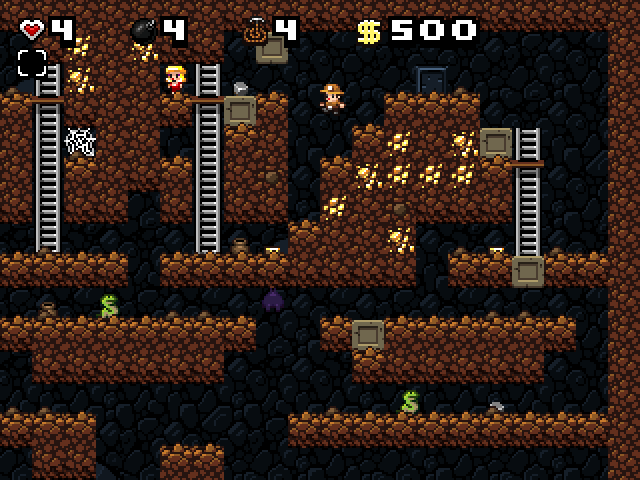
\includegraphics[width=.65\textwidth]{fig/spelunky-pc-screen.png}
\caption{\label{fig:spelunky-gameplay}Exemplo de partida de spelunky, mostrando
elementos do jogo como o jogador, a caverna, os inimigos, os tesouros, entre
outros.}
\end{figure}


%----------
\section{\label{section:spelunky-goals}Objetivos}
Apesar de o \textbf{objetivo principal} em Spelunky ser completar todos os
níveis, o jogo baseia a qualidade das partidas utilizando um sistema de
\textit{high scores}. Para tal, faz uso de uma série de métricas para
classificar os jogadores ao término de uma partida. Estas métricas são:

\begin{itemize}
	\item \textbf{Pontuação:} Mede a quantidade de tesouros obtidos pelo jogador
	no decorrer da partida. Existem diversos tipos de tesouros, como barras de
	ouro, pedras preciosas e estatuetas sagradas. Salvas as estatuetas sagradas,
	que devem ser carregadas até o fim do nível, o jogador precisa simplesmente
	tocar um tesouro para coletá-lo. Os tesouros se encontram espalhados pelo
	chão, dentro do terreno, dentro de baús ou são deixados por certos inimigos
	ao serem abatidos.

	\item \textbf{Tempo:} Mede o tempo para completar a partida. Começa a contar
	a partir do momento em que o jogador entra no primeiro nível e para de
	contar no fim do último nível. A contagem de tempo é interrompida durante as
	transições de nível e quando o jogador pausa a partida.

	\item \textbf{Abates:} Quantidade de inimigos abatidos pelo jogador durante
	a partida. Mortes acidentais de inimigos -- cair de um penhasco, acionar uma
	armadilha, etc. -- não aumentam este contador.

	\item \textbf{Salvamentos:} Quantidade de donzelas em perigo que foram
	resgatadas pelo jogador. Geralmente existe uma donzela em perigo por nível,
	mas existe a possibilidade -- mesmo que pequena -- de uma donzela não
	aparecer em alguns níveis. Para resgatar uma donzela, o jogador deve
	carregá-la com vida até a saída do nível.
\end{itemize}

Embora o jogo ofereça 4 métricas de classificação diferentes, a comunidade de
jogadores de Spelunky não mostra interesse significativo em atingir quantidades
elevadas de número de abates e número de salvamentos, se concentrando apenas em
atingir pontuações máximas e em concluir o jogo no menor tempo
possível\footnote{Comunidade de ranking de jogadores de Spelunky:
https://mosstier.com}. Pode-se concluir, portanto, que os \textbf{objetivos
secundários} mais importantes são a pontuação final e o tempo de partida. A
Figura \ref{fig:spelunky-scores} mostra um exemplo de pontuação final obtida.

\begin{figure}[htb!]
\centering
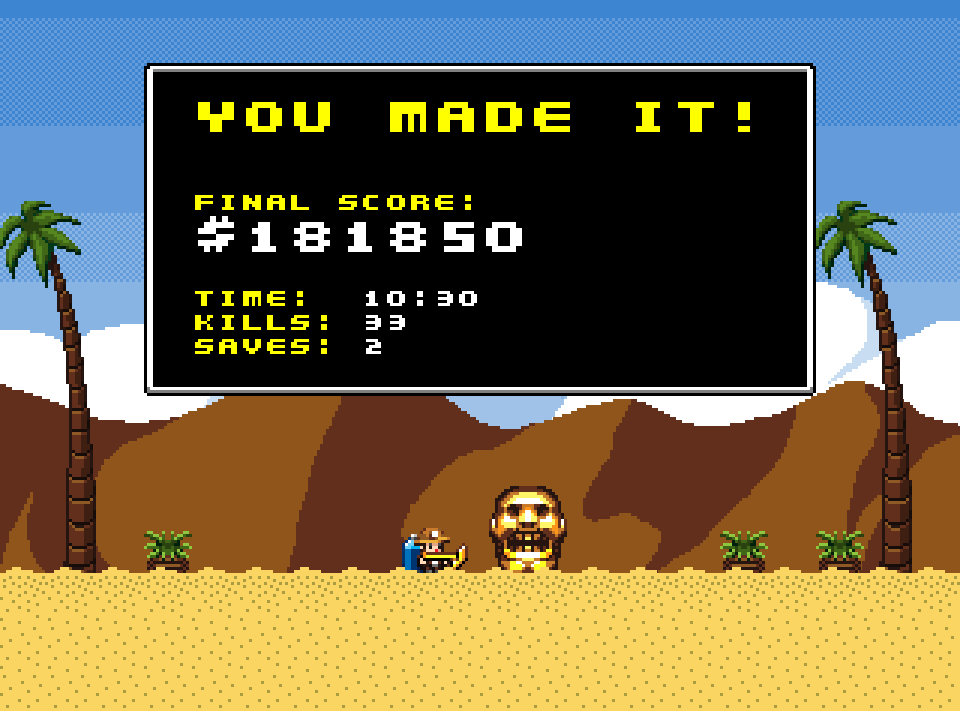
\includegraphics[width=.65\textwidth]{fig/spelunky-score.png}
\caption{\label{fig:spelunky-scores}Exemplo de pontuação final obtida ao fim de
uma partida de Spelunky.}
\end{figure}


%----------
\section{\label{section:spelunky-structure}Estrutura do jogo}
Uma partida de Spelunky é dividida em \textbf{níveis}, cada um sendo
representado por um mapa diferente. O jogador, ao entrar em um nível, é
posicionado na parte superior do mapa. Como não é informado ao jogador a posição
exata da saída, ele deve explorar o ambiente até encontrá-la. A saída sempre
está localizada em algum lugar na parte mais inferior do mapa. Ao utilizar a
saída, o jogador é enviado para o próximo nível e não pode retornar ao mapa que
acabou de completar.

O jogo é dividido em 4 \textbf{áreas} principais: \textbf{As Minas} (níveis 1 a
4), \textbf{A Selva} (níveis 5 a 8), \textbf{As Cavernas de Gelo} (níveis 9 a
12) e \textbf{O Templo} (níveis 13 a 16). Cada área possui um estilo de mapa e
aparência única. A dificuldade do jogo também aumenta gradativamente conforme o
jogador avança pelas áreas, principalmente porque os inimigos vão se tornando
cada vez mais fortes. O último nível do Templo é o \textbf{Covil de Olmec}. onde
o jogador deve enfrentar e derrotar \textbf{Olmec}. Após derrotar o inimigo
final, o explorador é recompensado com uma estatueta gigante feita de ouro e o
jogo termina.


\subsection{Atalhos}
É possível, ao iniciar uma partida, burlar este progresso entre áreas e ir
diretamente para as três ultimas áreas do jogo utilizando atalhos, criados pelo
personagem conhecido como \textbf{Homem do Túnel}. Para ter acesso a estes
atalhos, o jogador deve primeiramente auxiliar o Homem do Túnel a criá-los. O
personagem sempre aparece ao fim do último nível das primeiras três áreas do
jogo -- níveis 4, 8 e 12 --, se oferecendo para criar uma passagem secreta que
leva ao início da área que o jogador está prestes a chegar. Para criar a
passagem, o jogador deve ceder ao Homem do Túnel uma certa quantia de dinheiro.
O atalho da Selva, das Cavernas de Gelo e do Templo custam 100.000, 200.000 e
300.000, respectivamente.

Uma vez construídas, estas passagens são permanentes e podem ser acessadas ao
início de uma partida. Contudo, é importante ressaltar que, ao burlar etapas do
jogo, a pontuação do jogador não será contada para os \textit{high scores}. A
Figura \ref{fig:spelunky-tunnelman} ilustra a construção de um atalho e o acesso
aos atalhos antes do início da partida.

\begin{figure}[htb!]
\centering
	\begin{subfigure}[b]{0.4\textwidth}
		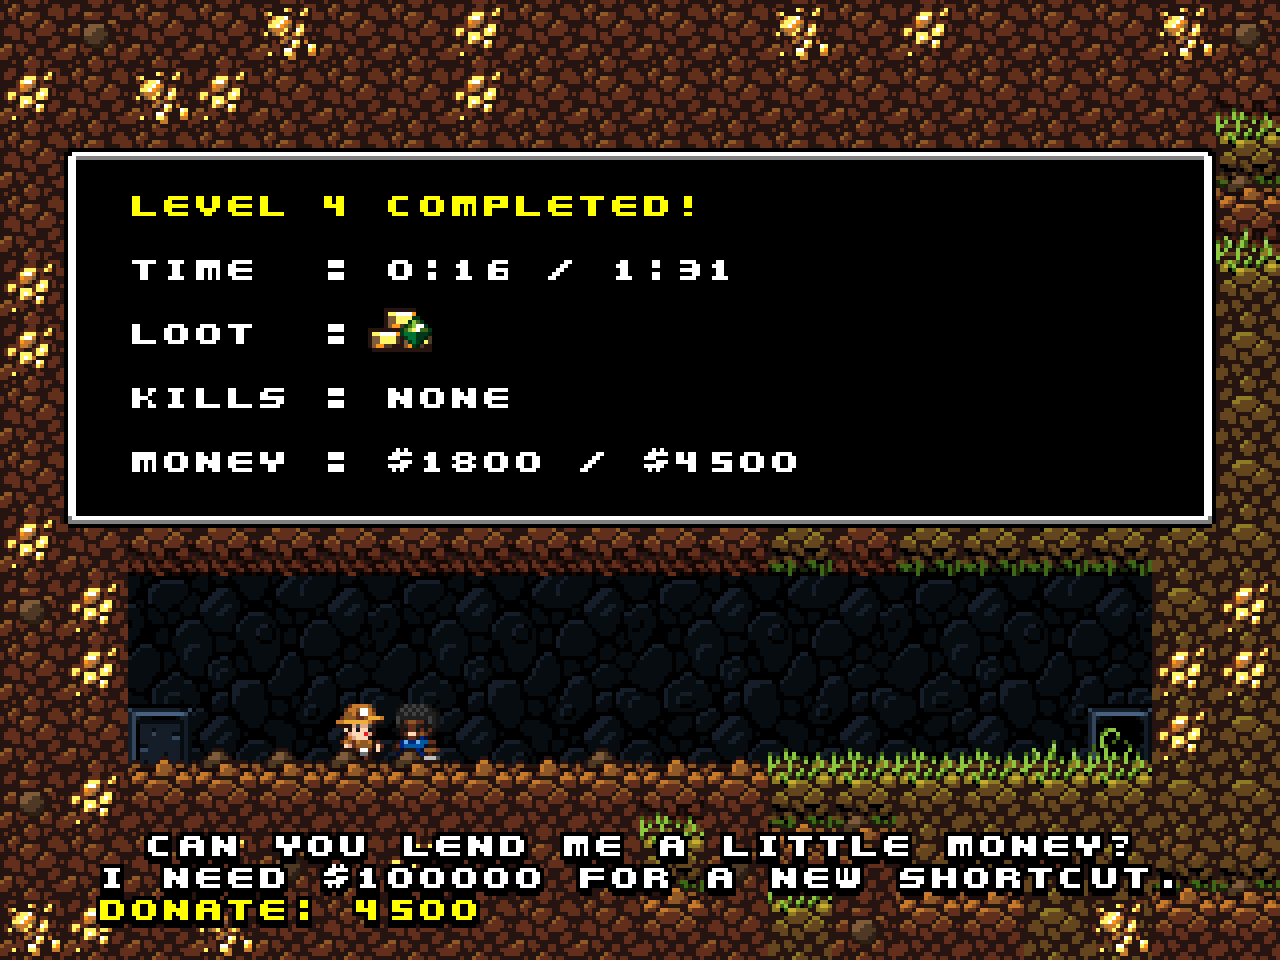
\includegraphics[width=\textwidth]{fig/spelunky-tunnelman.png}
		\caption{O Homem do Túnel solicitano ajuda para construir o atalho para
		a Selva.}
		\label{fig:spelunky-tunnelman}
	\end{subfigure}
	\begin{subfigure}[b]{0.4\textwidth}
		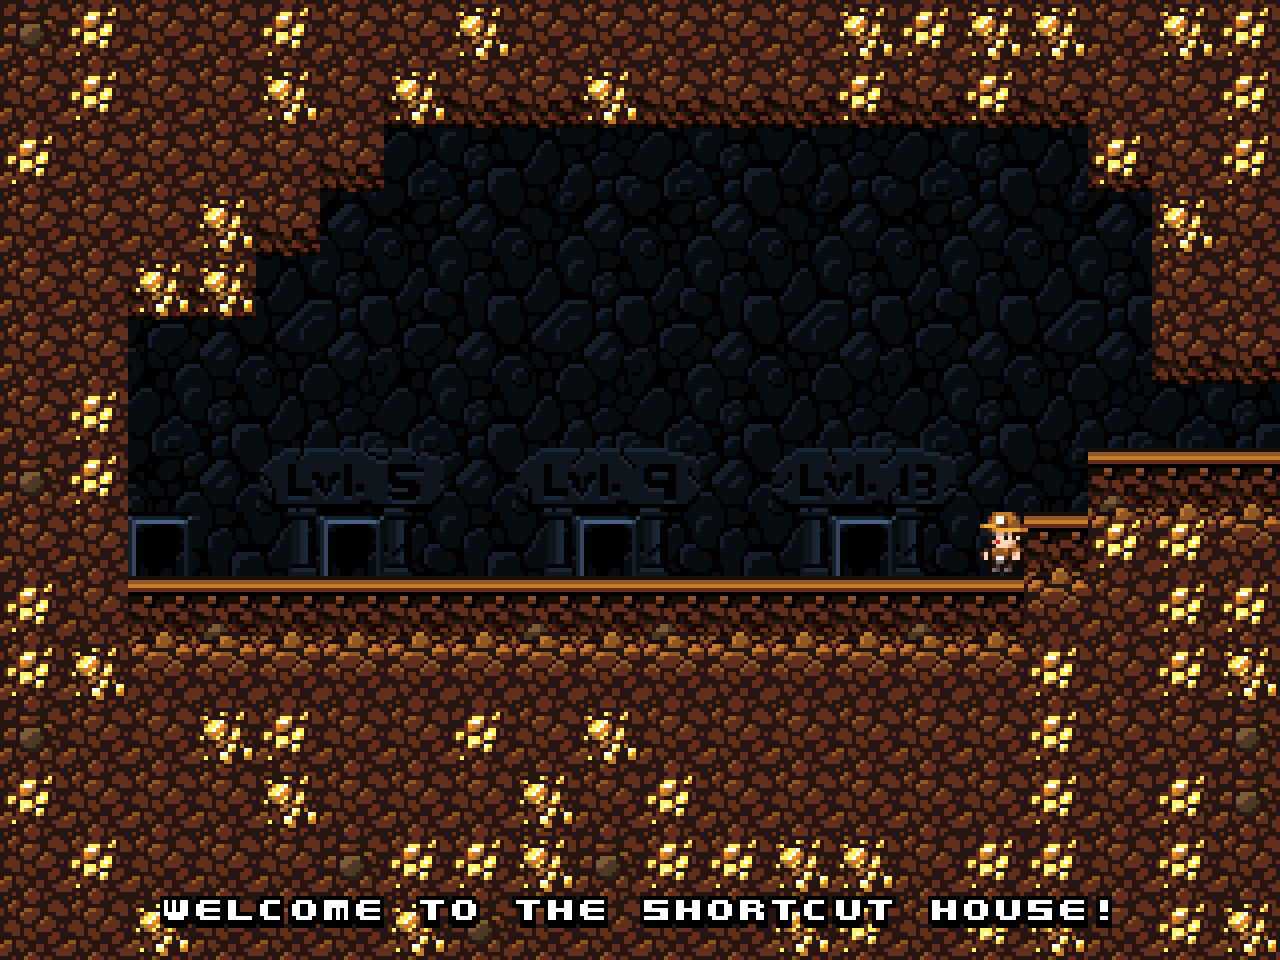
\includegraphics[width=\textwidth]{fig/spelunky-shortcuts.png}
		\caption{Os atalhos disponíveis antes do início da partida.}
		\label{fig:spelunky-shortcuts}
	\end{subfigure}
	\caption{Exemplo das interações com o Homem do Túnel e com os atalhos de
	\textit{Spelunky}.}
	\label{fig:spelunky-shortcuts-example}
\end{figure}


\subsection{Áreas Secretas}
Além das áreas principais, existem duas áreas secretas: \textbf{O Mercado Negro}
e \textbf{A Cidade de Ouro}. Estas áreas do jogo são fundamentais para se obter
equipamentos e grandes quantidadeds de tesouros, mas o jogador só obterá acesso
a elas se respeitar uma série de requisitos impostos pelo jogo. A Figura
\ref{fig:spelunky-secret-areas} exemplifica a aparência destas áreas secretas.

\begin{figure}[htb!]
\centering
	\begin{subfigure}[b]{0.4\textwidth}
		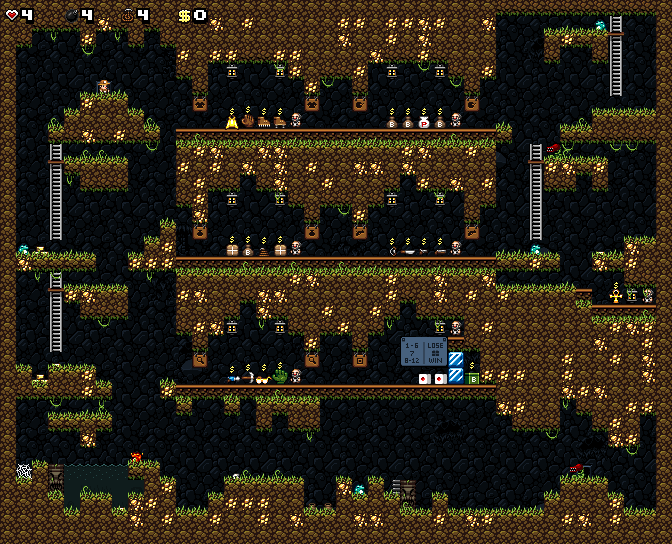
\includegraphics[width=\textwidth]{fig/spelunky-blackmarket.png}
		\caption{O Mercado Negro}
		\label{fig:spelunky-blackmarket}
	\end{subfigure}
	\begin{subfigure}[b]{0.4\textwidth}
		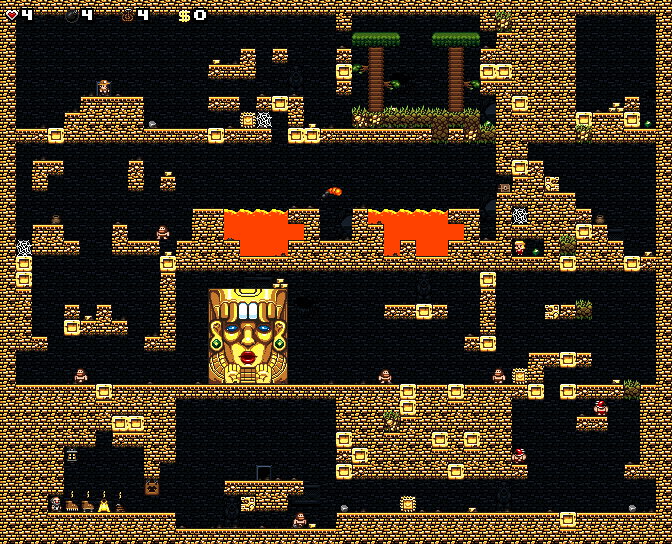
\includegraphics[width=\textwidth]{fig/spelunky-cityofgold.png}
		\caption{A Cidade de Ouro}
		\label{fig:spelunky-cityofgold}
	\end{subfigure}
	\caption{Exemplos das áreas secretas que podem ser acessadas pelo jogador em
	\textit{Spelunky}}
	\label{fig:spelunky-secret-areas}
\end{figure}


Para entrar no Mercado Negro, o jogador deve encontrar sua entrada -- que estará
oculta dentro do terreno do mapa -- enquanto explora a área da selva. O jogador
pode utilizar um item especial chamado \textbf{Udjat Eye} para ajudá-lo a
encontrar a entrada da área. O uso do item não é necessário, mas é aconselhável,
pois é quase impossível de localizar a entrada sem ele. Dentro do mercado negro,
o jogador encontrará vários comerciantes e terá a oportunidade de trocar seus
tesouros por equipamentos e itens diversos.

Entrar na Cidade de Ouro é muito mais complexo e é considerado um dos maiores
desafios do jogo, pois requer que o jogador colete uma série de artefatos
egípcios -- ilustrados na Figura \ref{fig:spelunky-artifacts} -- e execute uma
longa cadeia de ações ao longo da partida. A Cidade de Ouro é idêntica a um
nível do Templo, mas o terreno é feito de ouro maciço -- podendo ser destruído
com bombas -- e contém muito mais tesouros para coletar.  Além disso, o nível
contém uma estátua dourada gigante feita de ouro e pedras preciosas que pode ser
destruída pelo jogador. As etapas para entrar na Cidade de Ouro são:

\begin{enumerate}
	\item Coletar o \textbf{Udjat Eye}: O primeiro artefato se encontra dentro
	de um baú em algum nível da primeira área do jogo, as Minas. O jogador deve
	localizar a chave deste baú -- que se encontra no mesmo nível -- para poder
	abrí-lo. O Udjat Eye é capaz de encontrar a localização exata da entrada do
	Mercado Negro. O artefato pisca e brilha quanto mais próximo da entrada o
	jogador estiver, facilitando a localização da entrada.

	\item Coletar o \textbf{Ankh}: O segundo artefato se encontra no Mercado
	Negro e pode ser comprado (ou furtado) de um comerciante específico que
	vende somente este ítem. O Ankh oferece ao jogador uma segunda vida, caso
	venha a sucumbir.

	\item Coletar o \textbf{Hedjet}: O terceiro artefato pode ser obtido nas
	Cavernas de Gelo. Para obtê-lo, o jogador deve localizar um Moai\footnote{
	Estrutura monolítica com aparência humana. Os Moai foram esculpidos pelos
	Rapa Nui, habitantes nativos da Ilha de Páscoa.} e se morrer próximo a ele.
	O Ankh trará o jogador de volta a vida dentro do Moai e permitirá que o
	jogador colete o Hedjet.

	\item Coletar o \textbf{Cetro}: O quarto e último artefato podde ser obtido
	na última área do jogo, o Templo. O jogador deve encontrar e derrotar a
	Múmia, um dos inimigos mais fortes do jogo. Ao morrer, a múmia deixará o
	Cetro no chão. O Cetro é diferente dos outros itens porque, na verdade, é
	uma arma. Ele solta raios laser de cor rosa em formato de anel que perseguem
	e matam o inimigo mais próximo.

	\item Localizar a \textbf{Porta Dourada}: A última etapa do processo é
	encontrar a entrada da Cidade de Ouro, localizada em algum dos níveis do
	Templo. O jogador deve abandonar o Cetro e utilizá-lo como chave na Porta
	Dourada.
\end{enumerate}

\begin{figure}[htb!]
\centering

\includegraphics[width=.65\textwidth]{fig/spelunky-artifacts.png}
\caption{\label{fig:spelunky-artifacts}Os artefatos místicos de
\textit{Spelunky} necessários para acessar a Cidade de Ouro. Da esquerda para a
direita: o Udjat Eye, o Ankh, o Hedjet e o Cetro.}
\end{figure}

Não é necessário que o jogador acesse as duas áreas secretas do jogo durante uma
partida, mas as quatro áreas principais devem necessáriamente ser visitadas --
salvo quando o jogador fizer uso de um atalho, abrindo mão da validez de sua
pontuação. É importante ressaltar que o jogo conta com o conceito de
\textbf{morte permanente}, que faz com que o jogador, ao ter seus pontos de vida
esgotados, tenha que recomeçar o jogo desde seu início, perdendo todo o
progresso obtido até então.  A Figura \ref{fig:spelunky-run} ilustra a relação
entre as áreas e o progresso de uma partida de Spelunky.

\begin{figure}[htb!]
\centering
\begin{tikzpicture}[
    room/.style={
        regular polygon, regular polygon sides=4,
        draw=black, fill=white,
        text width=4.5em, text centered,
        minimum size=5mm,
        font=\small
    }
]
\matrix(rooms)[row sep=1cm, column sep=1cm]
{
    \node[room] (r1) {As Minas};            &
    \node[room] (r2) {A Selva};             &
    \node[room] (r3) {As Cavernas de Gelo}; &
    \node[room] (r4) {O Templo};            &

    \\
                                            &
    \node[room] (r5) {O Mercado Negro};     &
                                            &
    \node[room] (r6) {A Cidade de Ouro};    &
    \\
};
\draw[->,>=latex] (r1.east) -- (r2.west);
\draw[->,>=latex] (r2.east) -- (r3.west);
\draw[->,>=latex] (r3.east) -- (r4.west);

\draw[->,>=latex] ([xshift=-.5cm]r2.south) -- ([xshift=-.5cm]r5.north);
\draw[->,>=latex] ([xshift=.5cm]r5.north) -- ([xshift=.5cm]r2.south);

\draw[->,>=latex] ([xshift=-.5cm]r4.south) -- ([xshift=-.5cm]r6.north);
\draw[->,>=latex] ([xshift=.5cm]r6.north) -- ([xshift=.5cm]r4.south);
\end{tikzpicture}
\caption{\label{fig:spelunky-run}Relação entre as áreas de Spelunky durante uma
partida do jogo.}
\end{figure}

%----------
\section{\label{section:spelunky-controls}Controle do Personagem}
Os controles básicos em Spelunky são relativamente simples. Para se deslocar
pelo mapa, o jogador pode enviar comandos ao personagem para \textbf{caminhar},
\textbf{correr} e \textbf{pular}. O explorador também pode se \textbf{pendurar}
com as mãos na lateral de uma plataforma e subir e descer escadas. Como a
visibilidade do mapa é limitada a tela, o jogador pode \textbf{mover a câmera}
levemente na vertical ao \textbf{olhar para cima} ou se \textbf{agaixar},
aumentando sua visibilidade do ambiente. O explorador pode \textbf{utilizar
bombas e cordas} para auxiliar no deslocamento pelo nível. As bombas causam uma
explosão que elimina os inimigos e também desobstrui passagens. Já as cordas
permitem que o personagem atinja partes do mapa que não seriam acessíveis ao
pular, por estarem muito elevadas. Existe a possibilidade, também, de
\textbf{comprar itens} e \textbf{realizar apostas} com tesouros nas lojas dos
comerciantes.

A complexidade nos controles de Spelunky surge com a combinação de ações com
objetos, acessórios e equipamentos. O jogador pode \textbf{carregar um
item} em suas mãos e utilizá-lo quando desejar. O efeito depende do item
equipado atualmente. Por exemplo, se estiver carregando uma pedra, ele o
arremessará para longe. Se estiver segurando uma espingarda, ele realizará um
disparo. Os acessórios e equipamentos também modificam o funcionamento de ações.
Alguns acessórios podem fazer com que o personagem pule mais alto ou seja capaz
de se agarrar nas paredes. Portanto, é necessária atenção para os itens
coletados e equipados atualmente pelo explorador.


%----------
\section{\label{section:spelunky-procgen}Algoritmo de Geração Procedural de
Níveis}
Os níveis de Spelunky são gerados proceduralmente, ou seja, utiliza
um algoritmo capaz de gerar automáticamente os elementos que irão compor o
nível. Isto significa que não existe uma maneira de se memorizar estratégias
específicas de um mapa em Spelunky, pois ao início de cada partida o mapa é
gerado de maneira única e os tesouros, itens e obstáculos são dispostos de
maneira diferente, fazendo com que o jogador tenha que aprender a lidar com os
elementos do jogo de forma individual, combinar este conhecimento e estabelecer
uma estratégia para vencer seus obstáculos e ser bem sucedido.

O algoritmo de geração procedural de níveis de Spelunky é dividido em três
etapas: a \textbf{geração do caminho de solução}, a \textbf{geração de salas} e
a \textbf{disposição de entidades}.

\subsection{\label{section:spelunky-procgen-path}Geração do Caminho de Solução}
Cada nível em Spelunky é construído a partir de 16 \textbf{salas}, dispostas em
uma grade 4 por 4. Nesta etapa do algoritmo é escolhido o \textbf{caminho
solução} do nível, uma sequência de salas que formam um caminho desobstruído da
entrada até a saída. Primeiramente, o gerador escolhe uma das quatro salas da
parte superior para colocar a entrada do nível. Escolhido o local da entrada, o
algoritmo gera um caminho até a saída através de movimentos aleatórios para a
esquerda, para a direita e para baixo na grade de salas. Caso o gerador atinja
um dos extremos horizontais da grade, ele se desloca para baixo e inverte a
direção horizontal do movimento anterior. A saída do nível é colocada quando o
algoritmo chega na última linha da grade e tenta realizar um movimento para
baixo. Assim, a saída sempre se encontrará em uma das quatro salas da parte
inferior do mapa.

Todas as salas que fazem parte do caminho solução são transponíveis do início ao
fim sem o uso de bombas, cordas ou outros equipamentos. Além disso, sempre
possuem aberturas na esquerda e na direita. As salas em que o caminho realiza
uma descida possuem aberturas embaixo e as salas onde o caminho chega de uma
descida possuem aberturas em cima. Isto garante que haverá conectividade entre
todas as salas do caminho principal. Já as salas que não fazem parte do caminho
solução não possuem esta garantia, podendo ser completamente seladas e somente
acessíveis utilizando algum equipamento ou destruindo parte do terreno. Estas
salas fora do caminho solução também podem ser lojas, altares de sacrifício,
altares de ídolos dourados, entre outras. A Figura
\ref{fig:spelunky-procgen-path} exemplifica um resultado desta etapa do
algoritmo.

\begin{figure}[htb!]
\centering
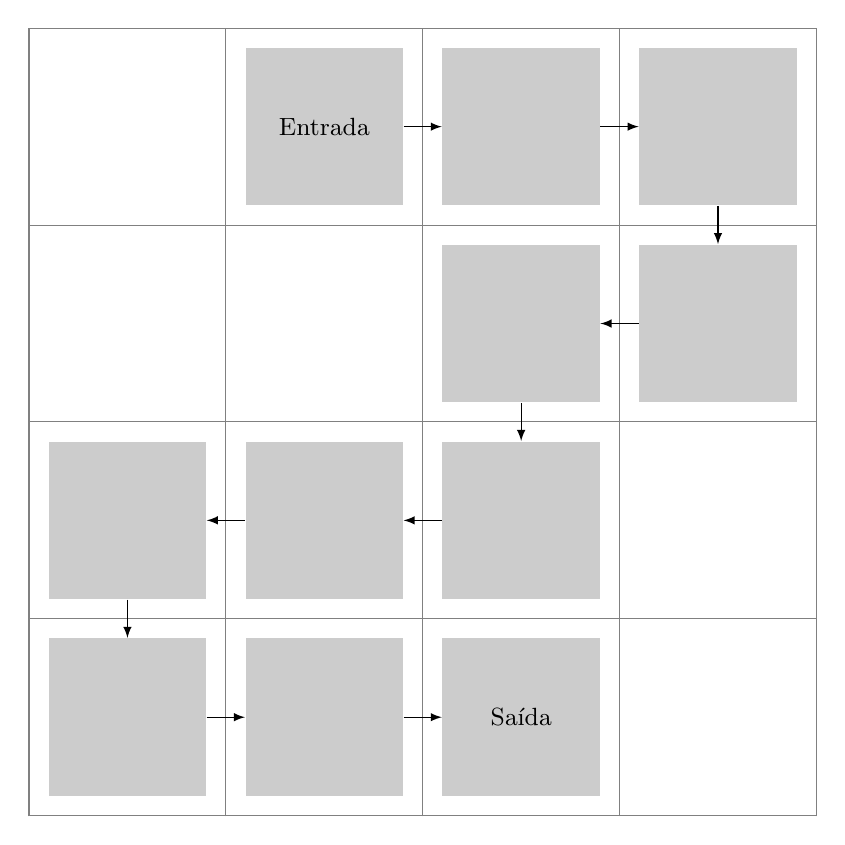
\begin{tikzpicture}[
    box/.style={
        rectangle,
        minimum width={2cm},
        minimum height={2cm},
        fill=gray!40,
        font=\small
    }
]
\draw[step=2.5cm, color=gray] (-5.01, -5.01) grid (5, 5);
\node [box] (b1) at ([xshift=1.25cm,yshift=-1.25cm]-2.5, 5) {Entrada};
\node [box] (b2) at ([xshift=1.25cm,yshift=-1.25cm]0, 5) {};
\node [box] (b3) at ([xshift=1.25cm,yshift=-1.25cm]2.5, 5) {};

\node [box] (b4) at ([xshift=1.25cm,yshift=-1.25cm]2.5, 2.5) {};
\node [box] (b5) at ([xshift=1.25cm,yshift=-1.25cm]0, 2.5) {};

\node [box] (b6) at ([xshift=1.25cm,yshift=-1.25cm]0, 0) {};
\node [box] (b7) at ([xshift=1.25cm,yshift=-1.25cm]-2.5, 0) {};
\node [box] (b8) at ([xshift=1.25cm,yshift=-1.25cm]-5, 0) {};

\node [box] (b9) at ([xshift=1.25cm,yshift=-1.25cm]-5, -2.5) {};
\node [box] (b10) at ([xshift=1.25cm,yshift=-1.25cm]-2.5, -2.5) {};
\node [box] (b11) at ([xshift=1.25cm,yshift=-1.25cm]0, -2.5) {Saída};

\draw[->,>=latex] (b1.east) -- (b2.west);
\draw[->,>=latex] (b2.east) -- (b3.west);

\draw[->,>=latex] (b3.south) -- (b4.north);
\draw[->,>=latex] (b4.west) -- (b5.east);
\draw[->,>=latex] (b5.south) -- (b6.north);

\draw[->,>=latex] (b6.west) -- (b7.east);
\draw[->,>=latex] (b7.west) -- (b8.east);
\draw[->,>=latex] (b8.south) -- (b9.north);
\draw[->,>=latex] (b9.east) -- (b10.west);

\draw[->,>=latex] (b10.east) -- (b11.west);
\end{tikzpicture}
\caption{\label{fig:spelunky-procgen-path}Exemplo de caminho solução gerado na
primeira etapa do algoritmo de geração procedural de níveis de Spelunky.}
\end{figure}

\subsection{\label{section:spelunky-procgen-rooms}Geração de Salas}
A próxima etapa do algoritmo é gerar separadamente as salas que irão compor o
nível. Para fazer isto, o gerador se baseia em \textit{layouts} de salas
pré-estabelecidos pelo desenvolvedor, sendo que cada tipo possui em torno de 6 a
12 \textbf{modelos}. Estes modelos são descritos através de sequências de
caracteres comuns. Uma sala em Spelunky é representada por uma grade 10 por 8 de
\textit{tiles}\footnote{Tipo de representação visual muito utilizada por jogos
2D para dispor os elementos de um jogo em forma de grade, onde cada elemento se
chama \textit{tile}.}, o que significa que cada modelo deve conter exatamente 80
caracteres. A Figura \ref{fig:spelunky-procgen-room-template} ilustra um exemplo
de modelo utilizado pelo gerador.

\begin{figure}[htb!]
\centering
\begin{tabular}{c c c c c c c c c c}
    0 & 0 & 0 & 0 & 0 & 0 & 0 & 0 & 1 & 1 \\
    0 & 0 & 6 & 0 & 0 & 0 & 0 & L & 0 & 4 \\
    0 & 0 & 0 & 0 & 0 & 0 & 0 & P & 1 & 1 \\
    0 & 0 & 0 & 0 & 0 & 0 & 0 & L & 1 & 1 \\
    0 & 0 & 0 & 0 & 0 & 0 & 0 & L & 1 & 1 \\
    0 & 0 & 0 & 0 & 0 & 0 & 0 & 0 & 1 & 1 \\
    0 & 0 & 0 & 0 & 0 & 0 & 0 & 0 & 1 & 1 \\
    1 & 1 & 1 & 1 & 1 & 1 & 1 & 1 & 1 & 1 \\
\end{tabular}
\caption{\label{fig:spelunky-procgen-room-template}Exemplo de modelo utilizado
para gerar uma sala de Spelunky.}
\end{figure}

Cada caractere possui um significado diferente, informando ao gerador que tipo
de \textit{tile} deve ser utilizado em sua posição. Eles podem ser
\textbf{estáticos} ou \textbf{probabilísticos}. Os estáticos sempre são
substituídos pelo seu \textit{tile} correspondente. Os caracteres ``1'' (bloco
sólido), ``L'' (escada) e ``P'' (escada com plataforma) são exemplos deste
tipo. Já os probabilísticos possuem uma chance de serem substituídos pelo seu
\textit{tile} correspondente ou por um espaço vazio. Os caracteres ``2'' (50\%
de chance de ocorrer um bloco sólido) e ``4'' (25\% de chance de ocorrer um
bloco de empurrar) são exemplos do segundo tipo.

Os caracteres ``5'' e ``6'' possuem uma característica especial. Eles não são
mapeados para um único \textit{tile}, e sim para um conjunto 5 por 3 de
\textit{tiles}, chamados de \textbf{obstáculos}. Estes conjuntos também utilizam
sequências de caracteres pré-definidos para descrever seu \textit{layout}.
Existem dois tipos de conjuntos, os aéreos e os terrestres. A diferença entre os
tipos de conjunto é simples: um conjunto terrestre deve ser colocado próximo ao
chão e um conjunto aéreo deve ser colocado no ar. Quando o gerador está
realizando a montagem da sala e detecta um caractere de obstáculo, ele realiza
uma substituição por um dos modelos disponíveis. A Figura
\ref{fig:spelunky-procgen-room-chunk} exemplifica um modelo de obstáculos.

\begin{figure}[htb!]
\centering
\begin{tabular}{c c c c c}
    0 & 1 & 1 & 1 & 0 \\
    0 & 2 & 2 & 2 & 0 \\
    0 & 0 & 0 & 0 & 0
\end{tabular}
\caption{\label{fig:spelunky-procgen-room-chunk}Exemplo de modelo de conjunto de
\textit{tiles} utilizado para gerar uma sala de Spelunky.}
\end{figure}

O uso destes conjuntos ajuda a aumentar a aleatoriedade dos \textit{layouts} das
salas, trazendo a sensação de uma variedade maior, mesmo que o número de modelos
de salas seja pequeno. O resultado da combinação do modelo da sala da
representada na Figura \ref{fig:spelunky-procgen-room-template} com o modelo de
obstáculos representado na Figura \ref{fig:spelunky-procgen-room-chunk} é
evidenciado na Figura \ref{fig:spelunky-procgen-room-combination}.

\begin{figure}[htb!]
\centering
\begin{tabular}{c c c c c c c c c c}
    0 & 0 & 0 & 0 & 0 & 0 & 0 & 0 & 1 & 1 \\
    0 & 0 & 0 & 1 & 1 & 1 & 0 & L & 0 & 4 \\
    0 & 0 & 0 & 2 & 2 & 2 & 0 & P & 1 & 1 \\
    0 & 0 & 0 & 0 & 0 & 0 & 0 & L & 1 & 1 \\
    0 & 0 & 0 & 0 & 0 & 0 & 0 & L & 1 & 1 \\
    0 & 0 & 0 & 0 & 0 & 0 & 0 & 0 & 1 & 1 \\
    0 & 0 & 0 & 0 & 0 & 0 & 0 & 0 & 1 & 1 \\
    1 & 1 & 1 & 1 & 1 & 1 & 1 & 1 & 1 & 1 \\
\end{tabular}
\caption{\label{fig:spelunky-procgen-room-combination}Exemplo de um modelo de
sala e um modelo de conjunto de \textit{tiles} utilizados para gerar uma sala de
Spelunky.}
\end{figure}

Com a descrição dos caracteres em mão, podemos realizar uma interpretação do
modelo ilustrado na Figura \ref{fig:spelunky-procgen-room-combination}. O modelo
descreve uma sala com chão, uma parede à direita, uma escada que leva a uma
pequena passagem, obstruída por um bloco de empurrar, e alguns blocos aéreos que
o jogador pode utilizar para se movimentar.

\subsection{\label{section:spelunky-procgen-entities}Disposição de Entidades}
A última etapa do algoritmo envolve a disposição dos inimigos, tesouros e
armadilhas. O algoritmo percorre todos os \textit{tiles} sólidos do nível a fim
de decidir se colocará uma entidade naquele local ou em suas proximidades.  Cada
tipo de entidade possui restrições diferentes:

\begin{description}
	\item[Inimigos]
	necessitam de espaços vazios acima ou abaixo do \textit{tile} sendo
	verificado atualmente. Inimigos não são colocados em locais muito apertados,
	dentro da água ou dentro da sala que contém a entrada do nível.

	\item[Tesouros]
	podem ser gerados acima de qualquer \textit{tile} sólido, mas a chance e
	valor do tesouro aumentam para locais apertados e em buracos no chão. Não
	são gerados perto da entrada e da saída.

	\item[Armadilhas]
	os requisitos variam muito de acordo com o tipo de armadilha, que podem ser
	espinhos, lança-flechas, pedregulhos, entre outros.
\end{description}

Cada entidade possui uma chance diferente de ocorrer a cada verificação, e as
probabilidades de ocorrência variam para cada área do jogo. Por exemplo, para
cada \textit{tile} na área das Cavernas, um morcego possui uma chance de 1.66\%
de ser gerado e um homem das cavernas possui uma chance de 0.12\% de ser gerado.
O algoritmo busca, através destas porcentagens, garantir que algumas entidades
apareçam mais frequentemente que outras, balanceando a dificuldade do jogo.

A Figura \ref{fig:spelunky-procgen-examples} exemplifica alguns níveis gerados
pelo algoritmo.

\begin{figure}[htb!]
\centering
	\begin{subfigure}[b]{0.4\textwidth}
		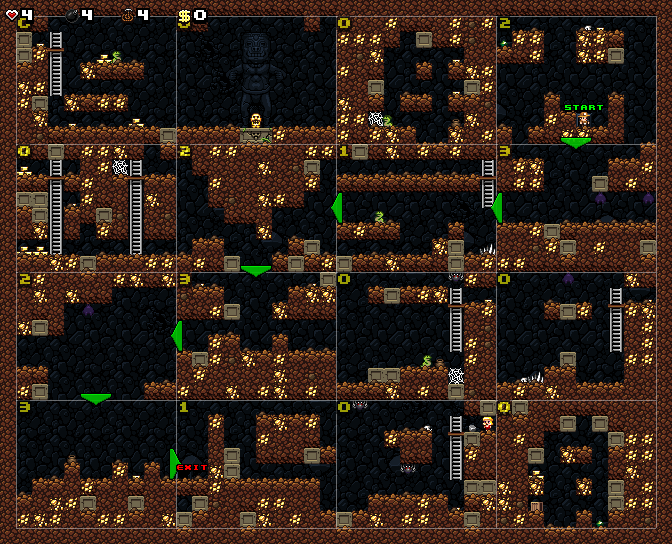
\includegraphics[width=\textwidth]{fig/spelunky-mines-example.png}
		\caption{As Minas}
		\label{fig:spelunky-mines-example}
	\end{subfigure}
	\begin{subfigure}[b]{0.4\textwidth}
		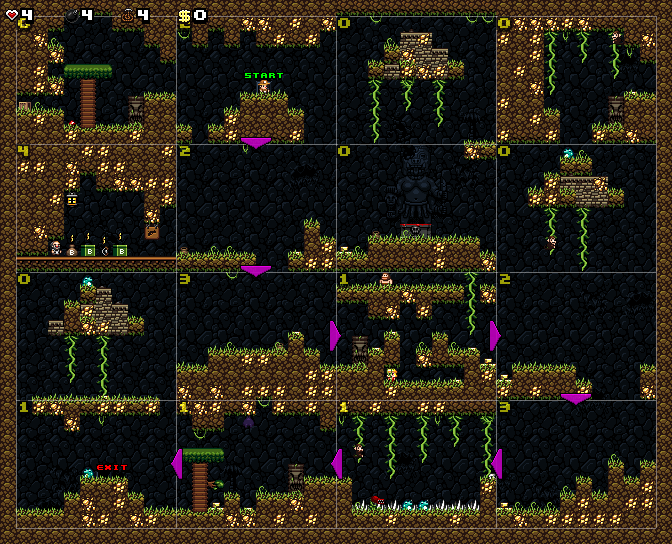
\includegraphics[width=\textwidth]{fig/spelunky-jungle-example.png}
		\caption{A Selva}
		\label{fig:spelunky-jungle-example}
	\end{subfigure}

	\begin{subfigure}[b]{0.4\textwidth}
		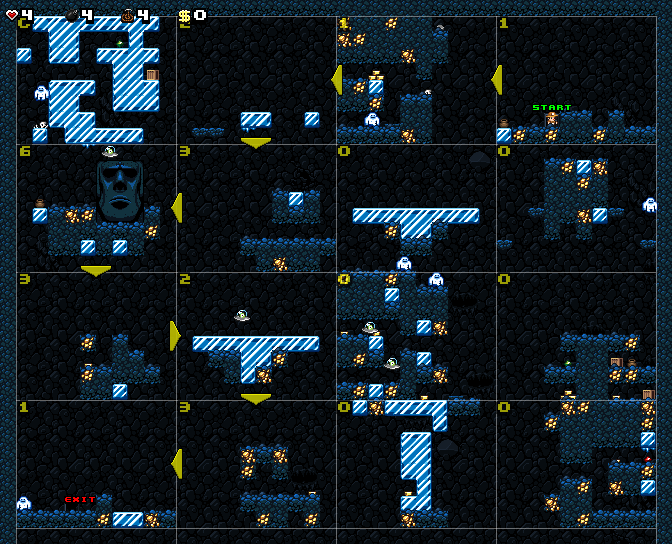
\includegraphics[width=\textwidth]{fig/spelunky-ice-example.png}
		\caption{As Cavernas de Gelo}
		\label{fig:spelunky-ice-example2}
	\end{subfigure}
	\begin{subfigure}[b]{0.4\textwidth}
		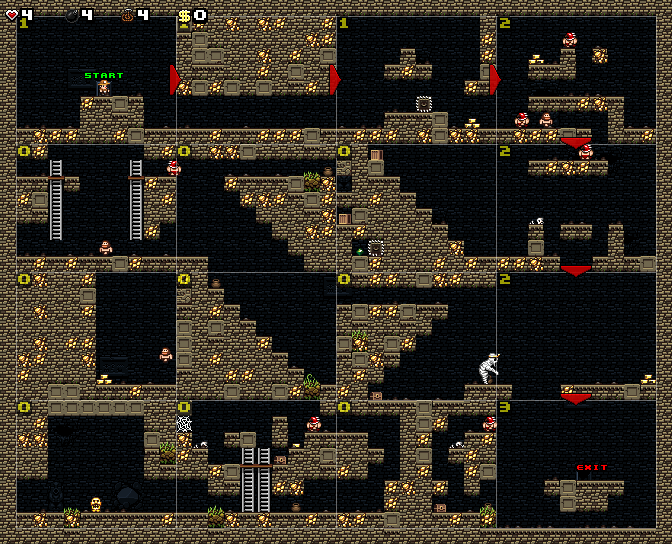
\includegraphics[width=\textwidth]{fig/spelunky-temple-example.png}
		\caption{O Templo}
		\label{fig:spelunky-temple-example}
	\end{subfigure}
	\caption{Exemplos do resultado final do algoritmo de geração de níves de
	\textit{Spelunky} para cada uma das áreas principais do jogo, com
	visualização da entrada, saída e caminho solução.}
	\label{fig:spelunky-procgen-examples}
\end{figure}


%----------
\section{\label{section:spelunky-obstacles}Obstáculos}
O universo de Spelunky é repleto de obstáculos, cujo único objetivo é impedir
que o jogador saia vivo de dentro das cavernas que está explorando. Estes
obstáculos podem ser \textbf{armadilhas} ou \textbf{monstros}. As armadilhas
são objetos projetados para punir invasores indesejados e os monstros são os
habitantes da caverna. Existem diversos tipos de armadilhas e monstros, e
alguns destes inclusive causam a morte instantânea do jogador. O anexo
\ref{section:spelunky-obstacles} apresenta a relação de monstros e
armadilhas, bem como uma breve descrição de seus comportamentos.

Além das armadilhas e monstros, o jogador também deve ter cuidado com os perigos
naturais presentes na caverna, como poços de lava e quedas de lugares muito
altos, pois também pode ser ferido por eles.


%----------
\section{\label{section:spelunky-items}Itens}
Em \textit{Spelunky}, existem diversos objetos com os quais o jogador pode
interagir para obter algum tipo de vantagem durante uma partida. Ao todo, são 43
itens diferentes, que são divididos nas seguintes categorias:

\begin{description}
	\item[Consumíveis]
	Objetos coletados pelo jogador que podem ser utilizados somente uma vez. Em
	alguns casos, o jogador pode carregar mais de um item consumível consigo.
	Alguns exemplo são as bombas, as cordas e o pára-quedas.

	\item[Acessórios]
	Equipamentos que, uma vez coletados pelo jogador, ficam disponíveis para uso
	durante toda a partida. Cada acessório oferece uma habilidade única que
	aumenta as chances de sobrevivência do explorador, e seus efeitos são
	manifestados ou passivamente -- sempre estão ativos -- ou através de uma
	ativação por parte do jogador. Alguns exemplos são o compasso, os sapatos de
	mola e a capa.

	\item[Armas]
	Equipamentos de combate de curto ou longo alcance carregados pelo explorador
	que o auxiliam a enfrentar os diversos monstros presentes na caverna. O
	jogador pode utilizar somente uma arma por vez, pois deve carregar a arma em
	suas mãos para utilizá-la. As armas não podem ser arremessadas pelo jogador.
	Alguns exemplos são o chicote, a espingarda e o arco.

	\item[Diversos]
	Objetos espalhados pela caverna que podem ser carregados e arremessados pelo
	jogador. Muitas vezes, servem como armas improvisadas, pois causam dano ao
	serem arremessadas e colidirem com algum inimigo. Também são utilizados para
	ativar armadilhas, impedindo que o jogador corra o risco de ativá-las sem
	querer. Alguns exemplos são as pedras, os vasos, as caixas e até mesmo
	corpos de inimigos abatidos. 
\end{description}

O anexo \ref{section:spelunky-obstacles} apresenta a relação de itens presentes
em \textit{Spelunky}, bem como uma breve descrição de seus comportamentos.


%----------
\section{\label{section:spelunky-dev}Desenvolvimento e Distribuição}
O jogo foi desenvolvido por Derek Yu -- utilizando o motor de desenvolvimento de
jogos \textit{GameMaker} (Versão 8.0 Pro) -- e lançado gratuitamente para a
plataforma \textit{Windows} em dezembro de
2008\footnote{https://forums.tigsource.com/index.php?topic=4017}. No fim de
2009, o criador optou por liberar o código fonte do jogo, permitindo sua
distribuição não-comercial e
modificação\footnote{http://www.spelunkyworld.com/files/COPYING.txt}. A
liberação do código fonte de Spelunky deve ser considerada um marco muito
importante, pois permitiu a criação de modificações para o jogo. Estas
modificações, normalmente encontradas no fórum oficial da
\textit{Mossmouth}\footnote{http://mossmouth.com/forums/index.php} -- empresa
desenvolvedora de jogos criada por Derek Yu --, são correções de \textit{bugs},
mapas customizados ou até mesmo modos de jogo completamente diferentes do jogo
original. Pode-se dizer que dar esta liberdade para a comunidade do jogo é um
dos fatores que ajuda a manter sua base de jogadores e atraem novos jogadores
até hoje.

O motor GameMaker disponibiliza diversas ferramentas que facilitam o trabalho
do desenvolvedor. Contando com funcionalidades como editores de
\textit{scripts}\footnote{Código desenvolvido para o controle dos
comportamentos dos elementos do jogo.} e de \textit{sprites}\footnote{Elementos
visuais do jogo, tais como o personagem, o fundo, os inimigos. Representados
como uma ou mais imagens, permitindo que as mesmas sejam animadas.},
gerenciadores de eventos, entre
outras\footnote{http://sandbox.yoyogames.com/downloads/docs/gmaker80.pdf}, o
GameMaker oferece um ótimo suporte ao desenvolvedor para a criação de jogos. O
motor disponibiliza uma linguagem de programação própria para seus
\textit{scripts}, a \textit{GameMaker Language}, ou \textit{GML}.

Em julho de 2012, a desenvolvedora \textit{Mossmouth} de Derek Yu lançou uma
versão remasterizada de \textit{Spelunky} para a plataforma \textit{Xbox 360},
nomeada \textit{Spelunky HD}. Esta nova versão possui ainda mais conteúdo que o
original, como novas áreas, monstros, itens, entre outros. Devido ao seu grande
sucesso, esta versão também foi posteriormente lançada para as plataformas
\textit{Windows}, \textit{PlayStation 3} e \textit{PlayStation Vita}. Este
trabalho, contudo, é focado na versão original de \textit{Spelunky}, também
conhecida como \textit{Spelunky Classic}.

\chapter{\label{chap:spelunkbots}SpelunkBots}

\begin{mdframed}[backgroundcolor=green!20]
\begin{itemize}
    \item
        Detalhar mais as informações recebidas pela API
    \item
        Listar e detalhar métodos da API
\end{itemize}
\end{mdframed}

Utilizando o código-fonte de Spelunky, Daniel Scales e Thomas Thompson, da
Universidade de Derby no Reino Unido, criaram o
\textit{SpelunkBots}\cite{SPELUNKBOTSPAPER}, um
\textit{framework} que permite a programação de \textit{bots} para o jogo
Spelunky. Um dos objetivos dos criadores é utilizar a aplicação para criar uma
competição de inteligência artificial para o jogo.

A \textit{API} possibilita que o desenvolvedor resgate informações de objetos
estáticos e dinâmicos contidos no ambiente do jogo, como o terreno, a
posição de tesouros, armadilhas e inimigos. Contudo, o objetivo da \textit{API}
disponibilizada por SpelunkBots é fazer com que a informação recebida pelo
\textit{bot} se assemelhe ao máximo com a percepção de um jogador humano.  Para
tal, o \textit{framework} implementa um sistema de \textit{fog of war},
limitando o conhecimento do ambiente que pode ser obtido pela inteligência
artificial. Para objetos estáticos, uma vez que o jogador visualizou o objeto,
ele poderá receber informações sobre ele permanentemente. Para objetos
dinâmicos, o \textit{bot} só poderá receber informações sobre eles se os mesmos
estiverem sendo visualizados por ele. A figura \ref{fig:spelunkbots-fow} ilustra
um exemplo de funcionamento do sistema, onde as áreas marcadas com o valor ``0''
representam um terreno transponível, enquanto as áreas com o valor ``1''
representam terreno intransponível. As áreas intransponíveis com o fundo
acinzentado correspondem ao sistema de \textit{fog of war}, cujas informações
não estão disponíveis pois tal área ainda não foi explorada pelo \textit{bot}.

\begin{figure}[htb!]
\centering
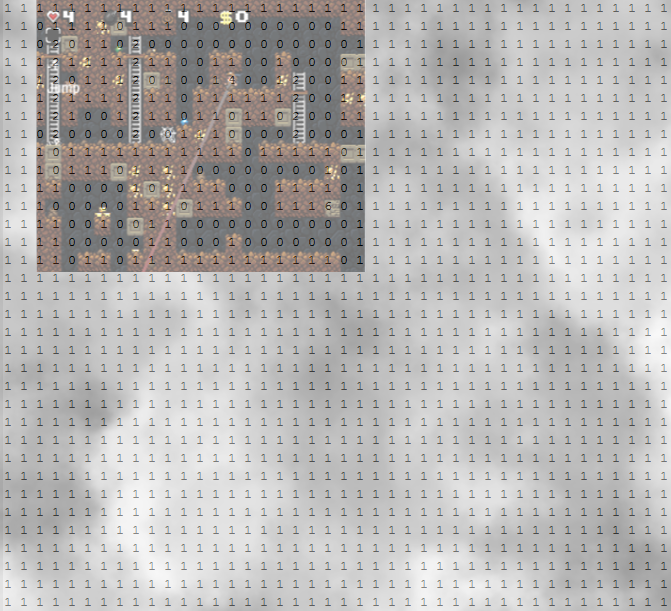
\includegraphics[width=.65\textwidth]{fig/spelunkbots-fow.png}
\caption {\label{fig:spelunkbots-fow}Visualização do sistema de \textit{fog of
war} demonstrando a diferença de informação recebida de elementos dentro e fora
do campo de visão do jogador.}
\end{figure}

\section{Utilização da \textit{API}}

É possível desenvolver \textit{bots} que fazem uso da \textit{API}
utilizando a linguagem GML (sigla para \textit{Game Maker Language}) ou
através da linguagem C++, ficando a critério do desenvolvedor a escolha da
linguagem. A única restrição que existe quanto ao uso de C++ dá-se no fato
de que a linguagem necessita de um processo de compilação através de uma
ferramenta externa, não sendo gerenciada diretamente pelo \textit{Game
Maker}. A figura \ref{fig:spelunkbots-usage-diagram} mostra a relação entre
o jogo, a \textit{API} e as possíveis linguagens de programação para se
utilizar. O código do Spelunky teve de ser modificado de forma a poder
interagir com o código do SpelunkyBots que, por sua vez, faz o uso de uma
solução de \textit{DLLs} escritas em C++ para fazer a interação com o jogo
através de código escrito em C++.

\begin{figure}[htb!]
\centering
\includegraphics[width=.65\textwidth]{fig/spelunkbots-usage-diagram.png}
\caption {\label{fig:spelunkbots-usage-diagram}Diagrama exibindo a relação
entre o jogo Spelunky, a API SpelunkyBots e as linguagens de programação que
podem ser usadas para a interação com o jogo.}
\end{figure}

A \textit{API} permite uma interação completa com o jogo através do uso
das variáveis expostas pelo
\textit{framework}\footnote{http://spelunkbots.com/wp-content/uploads/2015/02/SpelunkBots-API-A-Getting-Started-Tutorial.pdf}.
Com elas, é possível fazer o controle da movimentação do bot, bem
como identificar o tipo de terreno em que se está pisando e os inimigos que
aparecem em seu campo de visão. Além disso, também são disponibilizadas
informações sobre as armadilhas que podem atrapalhar o jogador. Por fim,
existem variáveis que permitem um melhor controle das informações relativas ao
\textit{bot}, como o posicionamento no eixo X e no eixo Y, se o \textit{bot}
encontra-se virado para a esquerda ou para a direita, entre outros. O uso dessas
variáveis torna possível a implementação de técnicas de inteligência artificial
no jogo Spelunky. O apêndice \ref{appendix:spelunkbots-variables} faz um
detalhamento maior de todas essas variáveis.

\chapter{\label{chap:theory}Fundamentação Teórica}
Neste capítulo, apresentaremos a base teórica necessária para compreender o
funcionamento das técnicas \textit{Behavior Trees} e \textit{NEAT}, escolhidas
para realizar o desenvolvimento dos agentes inteligentes de \textit{Spelunky}.

\begin{mdframed}[backgroundcolor=green!20]
\begin{itemize}
	\item
		Explicar a escolha das técnicas
\end{itemize}
\end{mdframed}


%----------
\section{\label{section:environment}Ambientes}
Todas as percepções e ações executadas por agentes racionais ocorrem no
\textbf{ambiente} no qual ele está inserido. A quantidade e variedade de
ambientes encontrados é vasta, mas é possível identificar dimensões (ou
características) de classificação para realizar uma categorização destes
ambientes. Estas características irão determinar que tipos de agentes --
enumerados na seção \ref{section:agents} -- são apropriados para cada ambiente.
As dimensões utilizadas para categorizar ambientes são:

\begin{description}
	\item[Observável, Parcialmente Observável ou Não-Observável]
		Um ambiente é observável se os sensores do agente lhe permitirem acesso
		completo ao estado do ambiente a cada ponto no tempo. Ambientes
		observáveis são convenientes, pois o agente não precisa manter um estado
		interno de conhecimento para se manter informado. O ambiente é
		parcialmente observável se os sensores do agente possuirem ruído ou não
		tiverem acesso completo ao ambiente. Se o agente não possuir nenhum tipo
		de sensor, então o ambiente é não-observável.

	\item[Agente Único ou Multi-Agente]
		Quando o agente não precisa interagir com nenhum outro agente no
		ambiente, então trata-se de um ambiente com agente único. Caso ele
		precise interagir de alguma forma (competição, cooperação ou
		comunicação) com outros agentes, então o ambiente é multi-agente.

	\item[Determinístico ou Estocástico]
		Se o próximo estado do ambiente for completamente determinado pela
		combinação do estado atual com uma ação executada pelo agente, então o
		ambiente é determinístico. Caso contrário, é estocástico.

	\item[Episódico ou Sequencial]
		Em ambientes episódicos, a experiência do agente é dividida em episódios
		atômicos, ou seja, são independentes entre sí. O agente não precisa
		pensar adiante pois, a cada episódio, recebe informações sensoriais e
		executa apenas uma ação, e o próximo episódio não será influenciado pela
		ação anterior. Já em ambientes sequenciais, a ação atual pode
		influenciar todas as decisões futuras, ou seja, ações a curto prazo
		podem ter consequências a longo prazo.

	\item[Discreto ou Contínuo]
		Ambientes discretos são aqueles onde se tem um número contável de ações
		e percepções possíveis. Em ambientes contínuos, o número de ações e de
		percepções muitas vezes são baseados em valores contínuos ou não são
		contáveis.

	\item[Conhecido ou Desconhecido]
		Esta distinção não se refere ao ambiente em sí, e sim sobre o
		conhecimento do agente (ou criador do agente) das "leis" de
		comportamento do ambiente. Em um ambiente conhecido, os resultados (ou
		probabilidades de resultados) das ações são conhecidos. Quando o
		ambiente é desconhecido, o agente precisa primeiro aprender como o
		ambiente funciona para saber fazer escolhas boas para atingir seus
		objetivos.
\end{description}


%----------
\section{\label{section:agents}Agentes Racionais}
Um agente é uma entidade que utiliza seus \textbf{sensores} para perceber o
ambiente no qual está inserido e interage através de seus \textbf{atuadores},
direcionando seus esforços para alcançar algum objetivo que se propõe a
atingir\cite[cap. 2]{RussellNorvig200912}. Um exemplo de agente racional é o ser
humano, que percebe o ambiente através de seus sentidos (visão, audição, entre
outros) e executa ações com seu corpo (braços, pernas, etc.). De acordo com
Russell \& Norvig\cite{RussellNorvig200912}, agentes racionais são agrupados nas
seguintes categorias: \textbf{agentes reflexivos}, \textbf{agentes baseados em
modelo}, \textbf{agentes baseados em objetivos} e \textbf{agentes baseados em
utilidade}.

Os \textbf{agentes reflexivos} são programados para executar ações baseadas em
algum evento percebido. Fica evidente que este tipo de agente simplesmente
executa uma ação baseado em suas percepções imediatas e não guardam informações
sobre suas experiências passadas, sendo apenas reativos.

Diferentemente dos agentes reflexivos, \textbf{agentes baseados em modelo} são
capazes de guardar informações sobre suas experiências passadas e sobre seu
estado atual. Este tipo de agente compreende como suas ações modificam o
ambiente onde está inserido e como o ambiente se altera independentemente de
suas ações, efetivamente construíndo um \textbf{modelo} do ambiente. 

Às vezes, ter conhecimento sobre o estado atual do ambiente não é suficiente
para decidir que ação executar. O agente precisa de alguma informação de que
situações são desejáveis, ou que objetivos desejar cumprir. Este é o caso de
\textbf{agentes baseados em objetivo}, que combinam um modelo do ambiente com
informações de objetivo para escolher as ações que mais o aproximam dos estados
desejáveis. A escolha de ações baseada em objetivos pode ser simples -- quando,
por exemplo, o objetivo é antigido com a execução de apenas uma ação -- ou
complexo -- quando, por exemplo, o agente deve considerar longas cadeias de
ações para atingir seus objetivos.

Em alguns casos, os objetivos não são suficientes para gerar comportamentos de
alta qualidade. Por exemplo, muitas vezes é possível atingir um objetivo através
de várias sequências de ações, mas algumas sequências são mais rápidas, mais
seguras, mais confiáveis ou mais baratas. Os \textbf{agentes baseados em
utilidade} fazem uso de uma função de utilidade para medir sua performance e,
assim, distinguir estados mais desejáveis e menos desejáveis. O agente, então, é
capaz de escolher as ações mais vantajosas para ele, aumentando sua performance.


%----------
\section{\label{section:machine-learning}Aprendizado de Máquina}
Quando queremos resolver um problema através de um programa de computador,
desenvolvemos um algoritmo que, dado uma entrada, executa uma sequência de
operações para fornecer uma resposta adequada para a tarefa em questão. Um
exemplo disso seriam os algoritmos para ordenação de números, onde a entrada é
um conjunto de números e a resposta é o conjunto ordenado. Para alguns
problemas, contudo, nem sempre é possível se chegar a um algoritmo que resolve
satisfatóriamente uma tarefa. Por exemplo, a tarefa de diferenciar
\textit{e-mails} de \textit{spam} e \textit{e-mails} legítimos é complexa, pois
os \textit{e-mails} de \textit{spam} estão mudando constantemente, e a
categorização de \textit{spam} pode variar de indivíduo para indivíduo. Assim,
criar manualmente um algoritmo para resolver esta tarefa pode ser extremamente
complexo ou até mesmo impraticável. A partir deste contexto, surgiu a área de
\textbf{aprendizado de máquina}, que estuda algoritmos que fornecem a programas
de computador a habilidade de aprender e se aperfeiçoarem, tornando-os capazes
de resolver tarefas sem serem explicitamente programados.

Existem três tipos principais de aprendizado de máquina\cite[cap.
18]{RussellNorvig200912}, que são diferenciados entre sí pelo tipo de
\textit{feedback} retornado pelo problema. Estas categorias são:
\textbf{aprendizado supervisionado}, \textbf{aprendizado não-supervisionado} e
\textbf{aprendizado por reforço}. No aprendizado supervisionado, é fornecido um
conjunto de dados com exemplos de entrada e resultados esperados para aquelas
entradas. Assim, a tarefa neste tipo de aprendizado consiste em aprender uma
função que mapeia entradas para saídas. No aprendizado não-supervisionado, o
programa recebe um conjunto de dados de entrada mas não recebe informações com o
tipo de saída esperado. O objetivo deste tipo de aprendizado geralmente é
detectar padrões em conjuntos de dados.  O último tipo de aprendizado, o
aprendizado por reforço, é diferente dos demais porque está diretamente ligado
ao conceito de agentes racionais.  Neste tipo de aprendizado, o agente interage
com um ambiente dinâmico e deve atingir algum objetivo. Quando o agente executa
ações no ambiente, é fornecido a ele algum tipo de retorno -- recompensas ou
punições --, para que ele possa aprender a agir da maneira correta a fim de
atingir seus objetivos.

Para agentes racionais, a capacidade de aprender fornece a oportunidade de se
tornar mais competente que o permitido pelo seu conhecimento inicial do problema
e do ambiente. Problemas como informação incompleta ou inexistente sobre o
ambiente são mais facilmente contornados, pois o agente será capaz de criar um
modelo de representação através do retorno obtido após a execução de ações.


%----------
\section{\label{section:neural-networks}Redes Neurais}
\begin{mdframed}[backgroundcolor=green!20]
\begin{itemize}
	\item
		Explicar
\end{itemize}
\end{mdframed}



%----------
\section{\label{section:environment}Algoritmos Evolutivos}
\begin{mdframed}[backgroundcolor=green!20]
\begin{itemize}
	\item
		Explicar
\end{itemize}
\end{mdframed}



%----------
\section{\label{section:behavior-trees}Behavior Trees}
A construção de bons agentes inteligentes depende fortemente da capacidade que
os agentes têm de tomar boas decisões de comportamento. No contexto de jogos
digitais, a partir da década de 90, a qualidade da inteligência artificial
passou a ser um diferencial no momento de compra de um jogo\cite[Cap.
1]{Millington:2009:AIG:1795711}, aumentando a importância da escolha de uma
técnica apropriada para desenvolver os agentes inteligentes.Das técnicas mais
populares, a \textbf{\textit{Behavior Tree}}, ou Árvore de Comportamento, é uma
das técnicas que mais se destaca, devido a sua \textbf{simplicidade} e
\textbf{extensibilidade}\cite[Cap.  4]{Rabin:2013:GAP:2566761}, e já foi
utilizada na indústria em jogos como \textit{Halo 2}\cite[Cap.
5]{Millington:2009:AIG:1795711} e
\textit{Spore}\footnote{http://chrishecker.com/My\_liner\_notes\_for\_spore},
por exemplo.

Uma \textit{Behavior Tree} é uma estrutura de dados baseada em árvore que contém
um nodo \textbf{raíz} (geralmente utilizada para controlar o fluxo inicial de
execução) e vários nodos filhos que representam os \textbf{comportamentos}. Cada
comportamento deve possuir uma \textbf{pré-condição} e uma \textbf{ação}. Caso a
pré-condição seja satisfeita, o agente poderá executar o comportamento descrito
pela ação do nodo\cite[Cap. 4]{Rabin:2013:GAP:256671}. Isto faz com que o
algoritmo de execução seja simples: partimos do nodo raíz em busca do primeiro
filho que satisfaça sua pré-condição (geralmente da esquerda para a direita). Ao
encontrá-lo, executamos sua ação. É importante ressaltar que somente um
comportamento é selecionado por vez. Portanto, se um comportamento for
selecionado, o algoritmo não tentará executar as ações dos nodos vizinhos na
mesma execução do algoritmo.

É possível adicionar estruturas de \textbf{controle de fluxo} a uma
\textit{Behavior Tree}. Desta forma, os ramos da árvore passam a ser usados para
controlar o fluxo de execução, enquanto os nodos-folha representam as
pré-condições e ações\cite[Cap. 10]{Rabin:2015:GAP:2821138}. Quando uma ação de
um nodo-folha é executado, ele informa ao seu pai (controlador de fluxo) o
estado de sua execução -- sucesso, falha ou em andamento. Existem diversos
tipos de estruturas de controle de fluxo que são utilizadas em \textit{Behavior
Trees}, mas as mais comuns são os de \textbf{seleção} e de \textbf{sequência}.

O algoritmo do controle de fluxo de seleção -- exemplificado no algoritmo
\ref{alg:behavior-tree-selection} -- faz a execução do \textbf{primeiro nodo
filho} que tiver sua pré-condição satisfeita. Quando termina de executar a ação
selecionada, aborta o procedimento, não visitando as demais ações.
Diferentemente do algoritmo de seleção, o algoritmo de \textbf{sequência} --
exemplificado no algoritmo \ref{alg:behavior-tree-sequence} -- tentará executar
\textbf{todos} os nodos que satisfizerem suas pré-condições de forma
\textbf{sequencial}. Sua execução só é interrompida quando não for possível
tomar a ação descrita pelo nodo ou quando não existirem mais nodos para se
avaliar.

\begin{algorithm}[H]
\begin{center}
	% Um exemplo de algoritmo utilizando a pacote 'algorithmic'
	%\algsetup{linenosize=\small,linenodelimiter=.}
	\begin{algorithmic}[1]
        \STATE filhos $\gets$ lista de nodos filhos
        \FOR{cada filho em filhos}
            \IF{filho.executar() == true}
                \RETURN true
            \ENDIF
        \ENDFOR
        \RETURN false
    \end{algorithmic}
\end{center}
\caption[Algoritmo para execução do controle de fluxo do tipo seleção em uma
behavior tree.]
{\label{alg:behavior-tree-selection} Algoritmo para execução do controle de
fluxo do tipo seleção em uma behavior tree.}
\end{algorithm}

\begin{algorithm}[H]
\begin{center}
	% Um exemplo de algoritmo utilizando a pacote 'algorithmic'
	%\algsetup{linenosize=\small,linenodelimiter=.}
	\begin{algorithmic}[1]
        \STATE filhos $\gets$ lista de nodos filhos
        \FOR{cada filho em filhos}
            \IF{filho.executar() == false}
                \RETURN false
            \ENDIF
        \ENDFOR
        \RETURN true
    \end{algorithmic}
\end{center}
\caption[Algoritmo para execução do controle de fluxo do tipo sequência em uma
behavior tree.]
{\label{alg:behavior-tree-sequence} Algoritmo para execução do controle de fluxo
do tipo sequência em uma behavior tree.}
\end{algorithm}

Para que fique mais claro como a técnica é utilizada, criamos um cenário
hipotético onde devemos criar a inteligência artificial de um agente (um robô
doméstico) que tem uma tarefa muito importante: limpar e organizar os móveis da
sala de estar de uma casa. Este robô, contudo, é movido à baterias, que não
duram muito. Então, de tempos em tempos, é necessário que ele recarregue suas
energias. Existem duas fontes de energia disponíveis para o robô: energia solar
e energia elétrica. A energia solar é preferível, por ser uma forma de energia
mais limpa, mas nem sempre é possível utilizá-la (um dia chuvoso, por exemplo).
A Figura \ref{fig:behavior-tree-example} representa o comportamento deste agente
através de uma \textit{Behavior Tree}. Para decidir entre as fontes de energia,
usamos um controle de fluxo do tipo \textbf{seleção}, pois somente um tipo de
energia deve ser utilizado. Já para executar suas tarefas (limpar e organizar),
usamos um controle de fluxo do tipo \textbf{sequência}, pois todas as tarefas
devem ser executadas.

\begin{figure}[H]
\centering
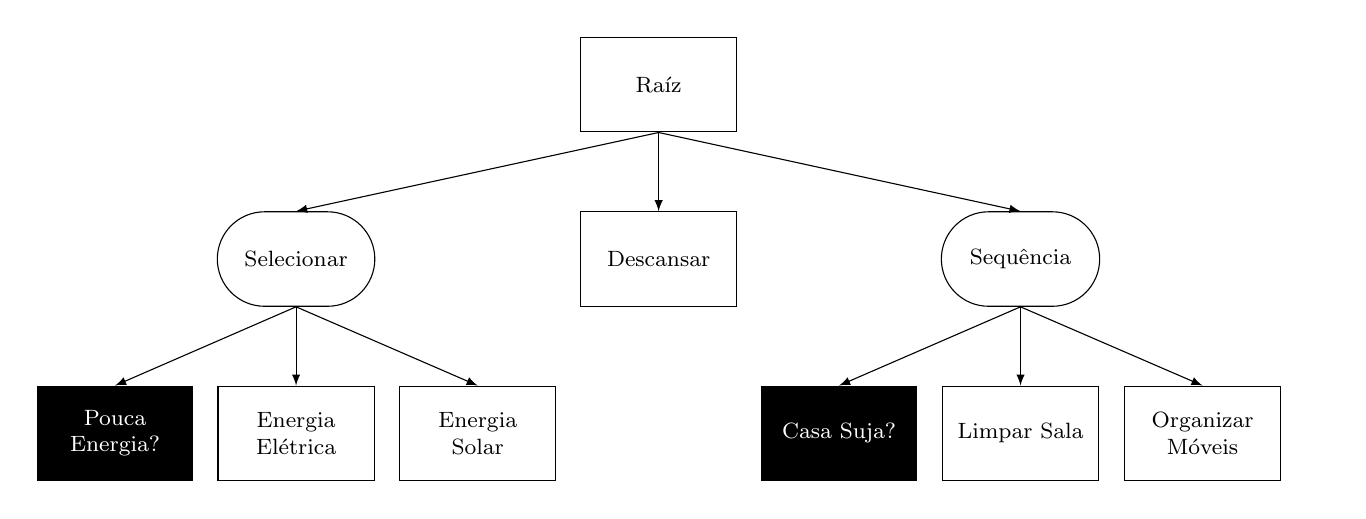
\begin{tikzpicture}[
    every node/.style={
        font=\footnotesize
    },
    composite/.style={
        minimum width=1.75cm, minimum height=1.2cm,
        text width=1.75cm,
        text centered,
        rounded rectangle,
        draw
    },
    action/.style={
        minimum width=1.75cm, minimum height=1.2cm,
        text width=1.75cm,
        text centered,
        rectangle,
        draw
    },
    precond/.style={
        minimum width=1.75cm, minimum height=1.2cm,
        text width=1.75cm,
        text centered,
        rectangle,
        fill=black,
        text=white
    }
]
\matrix [row sep=1cm, column sep=0.3cm] {
                                                &
                                                &
                                                &
    \node (n1)  [action]    {Raíz};             &
                                                &
                                                &
                                                &
    \\
                                                &
    \node (n2)  [composite] {Selecionar};       &
                                                &
    \node (n3)  [action]    {Descansar};        &
                                                &
    \node (n4)  [composite] {Sequência};        &
                                                &
                                                &
    \\
    \node (n5)  [precond]   {Pouca Energia?};   &
    \node (n6)  [action]    {Energia Elétrica}; &
    \node (n7)  [action]    {Energia Solar};    &
                                                &
    \node (n8)  [precond]   {Casa Suja?};       &
    \node (n9)  [action]    {Limpar Sala};      &
    \node (n10) [action]    {Organizar Móveis}; &
    \\
};
\draw[->,>=latex] (n1.south) -- (n2.north);
\draw[->,>=latex] (n1.south) -- (n3.north);
\draw[->,>=latex] (n1.south) -- (n4.north);

\draw[->,>=latex] (n2.south) -- (n5.north);
\draw[->,>=latex] (n2.south) -- (n6.north);
\draw[->,>=latex] (n2.south) -- (n7.north);

\draw[->,>=latex] (n4.south) -- (n8.north);
\draw[->,>=latex] (n4.south) -- (n9.north);
\draw[->,>=latex] (n4.south) -- (n10.north);
\end{tikzpicture}
\caption {\label{fig:behavior-tree-example}Exemplo de uma \textit{behaviour
tree} para representar um agente que deve carregar suas baterias caso seja
necessário, além de limpar e organizar a casa, descansando caso contrário.}
\end{figure}

Existem algumas outras técnicas que resolvem o mesmo problema que as
\textit{Behavior Trees} como, por exemplo, as \textbf{\textit{Finite State
Machines}} (máquinas de estados finitos), que são muito utilizadas em
inteligência artificial para jogos. Uma \textit{FSM} contém \textbf{estados} que
são ligados através de \textbf{transições}. Contudo, existem diversos problemas
com esta abordagem. A quantidade de estados e transições cresce
exponencialmente, os estados não podem ser reutilizados com facilidade e devemos
nos preocupar constantemente se existem transições inválidas no modelo. As
\textit{FSMs} possuem, resumidamente, um problema de modularidade.

Outra técnica muito utilizada são as \textbf{\textit{Hierarchical Finite State
Machines}} (máquinas de estados finitos hierárquicas). O objetivo da criação
desta técnica foi justamente mitigar alguns dos problemas das \textit{FSMs},
permitindo o englobamento de estados em uma hierarquia. Entretanto, o problema
de extensibilidade e praticidade ainda existem, porque ainda é baseada em
transições.


%----------
\section{\label{section:neat}NEAT}
% NEAT
% neuroevolução
% NEAT evolui os pesos e a rede em sí (TWEANNs)
% representação genética da rede
% problemas comuns em TWEANNs que o NEAT resolve
% (competing conventions, protecting innovation e initial population)

\begin{mdframed}[backgroundcolor=green!20]
\begin{itemize}
    \item
        Introdução: Escolha da técnica, história, paper
    \item
        Relação com aprendizado de máquina
    \item
        Relação com algoritmos genéticos
    \item
        Relação com redes neurais
    \item
        Explicação sobre a técnica: detalhamento de como funciona, termos
        técnicos, exemplos, pedaços de código (se necessário)
    \item
        Como será utilizada na construção dos \textit{bots}
\end{itemize}
\end{mdframed}

\chapter{\label{chap:related-work}Trabalhos Relacionados}
% MarI/O
% - https://www.youtube.com/watch?v=qv6UVOQ0F44 
% - https://www.youtube.com/watch?v=iakFfOmanJU 
% - https://www.youtube.com/watch?v=S9Y_I9vY8Qw 

% Atari DeepMind
% - http://arxiv.org/pdf/1312.5602v1.pdf  

% NERO
% - http://nn.cs.utexas.edu/?stanley:ieeetec05 

\section{N.E.R.O: Neuro-Evolving Robotic Operatives}

\begin{mdframed}[backgroundcolor=green!20]
\begin{itemize}
    \item
        O que é
    \item
        Técnica utilizada (citar paper)
    \item
        Relevância com o nosso trabalho
\end{itemize}
\end{mdframed}

%----------
\section{Playing Atari with Deep Reinforcement Learning}
O artigo apresenta um modelo de \textit{deep learning} capaz de aprender
políticas de controle para sete jogos do \textit{console} Atari 2600, criando
uma inteligência artificial capaz de jogar eficientemente todos os jogos,
inclusive superando jogadores humanos em alguns deles. O modelo utiliza
aprendizado por reforço e uma rede neural convolucional treinada com um variante
de \textit{Q-learning} para criar o agente.

Para criar estas políticas de controle, os autores utilizaram uma plataforma de
testes de inteligência artificial chamada \textit{Arcade Learning Environment}.
A cada passo de execução, o agente interage com o emulador, recebendo
informações do estado do jogo e enviando os comandos que deseja executar. As
informações recebidas eram um vetor dos \textit{pixels} apresentados na tela, o
conjunto de de ações possíveis para o jogo em questão e um valor de recompensa
quando a pontuação do jogo era alterada.

Como as informações do estado do jogo eram altamente dimensionais -- 33600
\textit{pixels} de informação visual --, foi necessário realizar um
pré-processamento para reduzir a dimensionalidade do estado do jogo -- reduzindo
para 7600 \textit{pixels}. Mesmo com esta redução, as quantidade de informações
recebidas ainda era considerável. Por isto, a utilização de \textit{deep
learning} e redes neurais convolucionais provou ser uma excelente -- e
necessária -- escolha para realizar o treinamento do agente. Contudo, o
treinamento do agente utilizando esta técnica é extremamente demorado.

Como a dimensionalidade do estado do jogo fornecido pela ferramenta
\textit{SpelunkBots} não é tão grande quanto a do trabalho em questão, optamos
por não fazer uso de \textit{deep learning}, mesmo que a técnica também seja
muito promissora.


%----------
\section{MarI/O}

Em junho de 2015, o canal do \textit{YouTube}
SethBling\footnote{https://www.youtube.com/user/sethbling/about} -- conhecido
por publicar vídeos de modificações de jogos como Mario e Minecraft -- divulgou
o vídeo \textit{MarI/O - Machine Learning for Video
Games}\footnote{https://www.youtube.com/watch?v=qv6UVOQ0F44}, que mostra um
jogador muito habilidoso completando o nível \textit{Donut Plains 1} de
\textit{Super Mario World}. É explicado, então, que o jogador em questão não é
humano, mas sim um programa de computador. Utilizando um emulador de
\textit{consoles} chamado
\textit{BizHawk}\footnote{http://tasvideos.org/BizHawk.html}, a linguagem de
programação \textit{Lua} e uma técnica de inteligência artificial chamada
\textit{\textbf{N.E.A.T}} (\textit{NeuroEvolution of Augmenting Topologies})
\cite{stanley:ec02} -- explicada detalhadamente no capítulo \ref{chap:neat} --,
o autor programou um \textit{bot} capaz de aprender como jogar o nível em
questão do início ao fim com sucesso. Como é explicado no vídeo, inicialmente o
\textit{bot} não conhecia absolutamente nada sobre como jogar \textit{Super
Mario World}. Contudo, através de várias simulações, adquiriu o conhecimento
necessário para superar todos os obstáculos presentes no nível.

\begin{figure}[htb!]
\centering
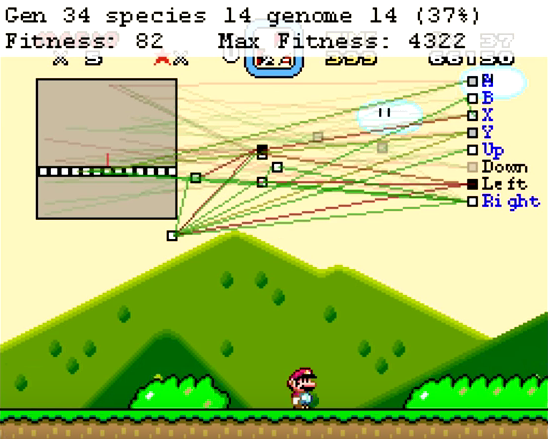
\includegraphics[width=.65\textwidth]{fig/mar-io-example.png}
\caption{\label{fig:mar-io-example}Exemplo da visão do jogo \textit{Super
Mario World} através do projeto \textit{MarI/O}, mostrando elementos de
controle usados pelo NEAT, como a rede neural, as possíveis ações, as
gerações, as espécies, os genomas, entre outros.}
\end{figure}

Depois do sucesso no nível \textit{Donut Plains 1}, o autor realizou mais
experimentos da aplicação da técnica
\textit{NEAT}\footnote{https://www.youtube.com/watch?v=iakFfOmanJU}
\footnote{https://www.youtube.com/watch?v=S9Y\_I9vY8Qw}. Inicialmente, testou em
dois outros níveis de \textit{Super Mario World}. Em \textit{Donut Plains 4}, o
processo de aprendizagem foi complicado, pois para obter progresso no nível era
necessário que aprendesse a interagir com certos elementos do mapa, e o autor
decidiu abortar o processo de aprendizagem. Já em \textit{Yoshi's Island 1},
obteve sucesso e foi capaz de concluir o nível. Com os testes finalizados, o
autor decidiu aplicar a técnica em outros dois jogos da franquia \textit{Mario}.
Em \textit{Super Mario Bros}, o \textit{bot} concluiu o primeiro nível e,
surpreendentemente, foi capaz de descobrir um \textit{glitch} no jogo que o
permitia passar por um segmento do segundo nível com maior rapidez. Em
\textit{Super Mario Kart}, depois de receber treinamento, o \textit{bot} foi
capaz de terminar uma corrida no nível \textit{Mario Circuit 1} em primeiro
lugar contra outros jogadores controlados pelo computador -- na dificuldade mais
fácil do jogo.

O \textit{MarI/O} é especialmente interessante e relevante porque tem um
objetivo muito similar ao deste trabalho: criar uma inteligência artificial
capaz de jogar uma partida de um jogo. Contudo, nos jogos escolhidos por
SethBling, os níveis são sempre os mesmos, o que torna mais fácil medir o
desempenho de um \textit{bot}, pois a disposição do nível é sempre igual e o
objetivo final sempre se encontra no mesmo lugar. Este não é o caso em
\textit{Spelunky}, onde os níveis são gerados proceduralmente. Além disso, os
níveis de \textit{Super Mario World} e \textit{Super Mario Bros.} são
essencialmente horizontais, e movimentar o personagem para a direita quase
sempre garante alguma forma de progresso. Isto facilita ainda mais o processo de
treinamento dos \textit{bots}. Em \textit{Spelunky} não é possível saber de
antemão onde se encontra a saída do nível e o movimento horizontal não garante o
progresso, visto que os níveis não são essencialmente horizontais. Estes fatores
influenciam na dificuldade de realizar o treinamento dos \textit{bots}.

\chapter{\label{chap:modeling}Modelagem}
O objetivo deste capítulo é, com base na fundamentação teórica apresentada no
Capítulo \ref{chap:theory} e em uma série de limitações impostas pelo
\textit{framework SpelunkBots}, indicar nossas escolhas de modelagem para
desenvolver os agentes inteligentes jogadores de \textit{Spelunky}.

Na seção \ref{section:spelunkbots-limitations}, apresentamos as limitações
impostas pelo \textit{framework SpelunkBots} que encontramos ao longo do
desenvolvimento deste trabalho. Em seguida, nas seções
\ref{section:modelling-vision} e \ref{section:modelling-outputs}, destacamos as
restrições de visão e ações disponíveis que escolhemos para facilitar o
treinamento dos agentes. Após, na seção \ref{section:modelling-network},
descrevemos as configurações das redes neurais utilizadas. Por fim, nas seções
\ref{section:modelling-genetic} e \ref{section:modelling-fitness}, detalhamos as
configurações utilizadas para o algoritmo genético do \textit{NEAT} e as funções
de aptidão utilizadas para realizar o treinamento dos agentes.


%----------
\section{\label{section:spelunkbots-limitations}Limitações do
\textit{SpelunkBots}}
Uma das partes centrais de nosso trabalho é o uso do \textit{framework}
\textit{SpelunkBots} para realizar a comunicação dos agentes inteligentes com o
jogo \textit{Spelunky}. Contudo, esta ferramenta possui algumas limitações
importantes de serem ressaltadas, pois elas afetam diretamente umas as outras e
causam um impacto significativo de performance de execução:

\begin{description}
	\item[Aceleração de Execução]
		Apesar de a ferramenta disponibilizar um mecanismo para permitir a
		aceleração da execução do jogo (através dos botões \textit{PageUp} e
		\textit{PageDown}), este efeito não pôde ser verificado quando
		realizamos alguns testes iniciais na ferramenta.

	\item[Contagem de Tempo]
		A contagem do tempo de execução de um nível é feito por fora do jogo,
		através de chamadas da função \textit{GetTickCount} do \textit{Windows}.
		Isto resulta em pelo menos dois efeitos colaterais. O primeiro é que se,
		por exemplo, pausarmos a execução do jogo e retormarmos a execução após
		um tempo, este intervalo de tempo será contabilizado como tempo de
		execução. O segundo é que se, por qualquer motivo, o jogo sofrer uma
		queda de desempenho momentânea (mais processamento de CPU, por exemplo),
		a contabilização do tempo continuará igual, o que significa que máquinas
		com capacidade de processamento inferiores não possuem, realisticamente
		falando, o mesmo tempo de execução que máquinas mais potentes.

	\item[Chamadas de DLL]
		Devido às limitações de programação externa oferecidas pelo
		\textit{GameMaker} como, por exemplo, a compatibilidade de chamada de
		funções	externas somente com tipo de retorno \textit{double} e
		\textit{char*}, a ferramenta precisa realizar várias chamadas de
		\textit{DLL} por etapa de execução para atualizar suas variáveis. Isto
		afeta a performance, resultando em um péssimo desempenho e código não
		otimizado.

	\item[Execução com Gráficos]
		Atualmente, é impossível executar a ferramenta sem janela gráfica, o que
		significa que, a cada certo período de tempo, é preciso renderizar o
		jogo. Durante o o treinamento dos agentes, essa função é desnecessária,
		ou seja, gasta-se tempo e capacidade de processamento para uma
		funcionalidade que não é utilizada.

	\item[Sistema Operacional]
		A ferramenta \textit{SpelunkBots} foi desenvolvida somente para a
		plataforma \textit{Windows}, o que significa que, para executá-la em
		outras plataformas (no nosso caso, \textit{Linux}), é preciso utilizar
		programas adicionais para realizar a compilação e execução do jogo. Este
		\textit{overhead} adicional prejudica o desempenho da aplicação.
\end{description}


%----------
\section{\label{section:modelling-vision}Visão do Agente}
Conforme detalhado anteriormente na Seção \ref{section:spelunkbots-information},
É possível receber informações de nodos do mapa, inimigos e objetos durante a
execução do jogo. Como nosso objetivo é tratar somente o domínio de navegação,
estamos interessados apenas nas informações de nodos do mapa. Devido ao sistema
de \textit{fog of war} (Figura \ref{fig:spelunkbots-fow}), não temos acesso
ilimitado às informações do mapa, restringindo-nos apenas a nodos que o jogador
já visualizou.

Contudo, seria inviável utilizar toda a visão disponível por três motivos. O
primeiro motivo é que estamos utilizando uma rede neural com número de entradas
fixa, então não é possível adicionar novos nodos de entrada durante a execução
do programa. O segundo motivo é que utilizar um número de entradas muito grande
resultaria em uma rede com muitas ligações, o que implicaria em uma necessidade
maior de tempo de processamento. O terceiro e último motivo é que, dadas as
limitações da ferramenta \textit{SpelunkBots} apresentadas na seção
\ref{section:spelunkbots-limitations}, identificamos que devemos buscar pela
simplicidade, pois caso contrário a performance dos agentes será afetada.

Outra questão importante é identificar quais são os tipos de nodos que são
interessantes para o domínio da navegação. Nodos como, por exemplo, o altar de
sacrifício, ou armadilhas de flechas não são pertinentes ao problema que
desejamos tratar inicialmente. Já nodos como o chão escorregadio ou a armadilha
de lanças apresentam grandes desafios a serem superados, e é provável que não
seja uma boa ideia considerá-los originalmente.

Optamos, portanto, por limitar a visão do agente em dois aspectos:

\begin{itemize}
	\item \textbf{Região de Visão:} o agente só será capaz de receber
		informações de nodos em sua proximidade, em uma região quadrada ao seu
		redor. A Figura \ref{fig:vision-limitation} ilustra um exemplo de região
		de visão dos agentes.

	\item \textbf{Tipos de Nodo:} limitamos os tipos de nodo que o agente é
		capaz de visualizar, permitindo somente nodos dos tipos: vazio, terreno
		, saída, escada e espinho. Caso o agente visualize qualquer outro tipo
		de nodo durante a execução, ele o interpretará como um nodo do tipo
		terreno. A Figura \ref{fig:vision-nodes} ilustra os nodos que o agente é
		capaz de enxergar.
\end{itemize}

\begin{figure}[htb!]
\centering
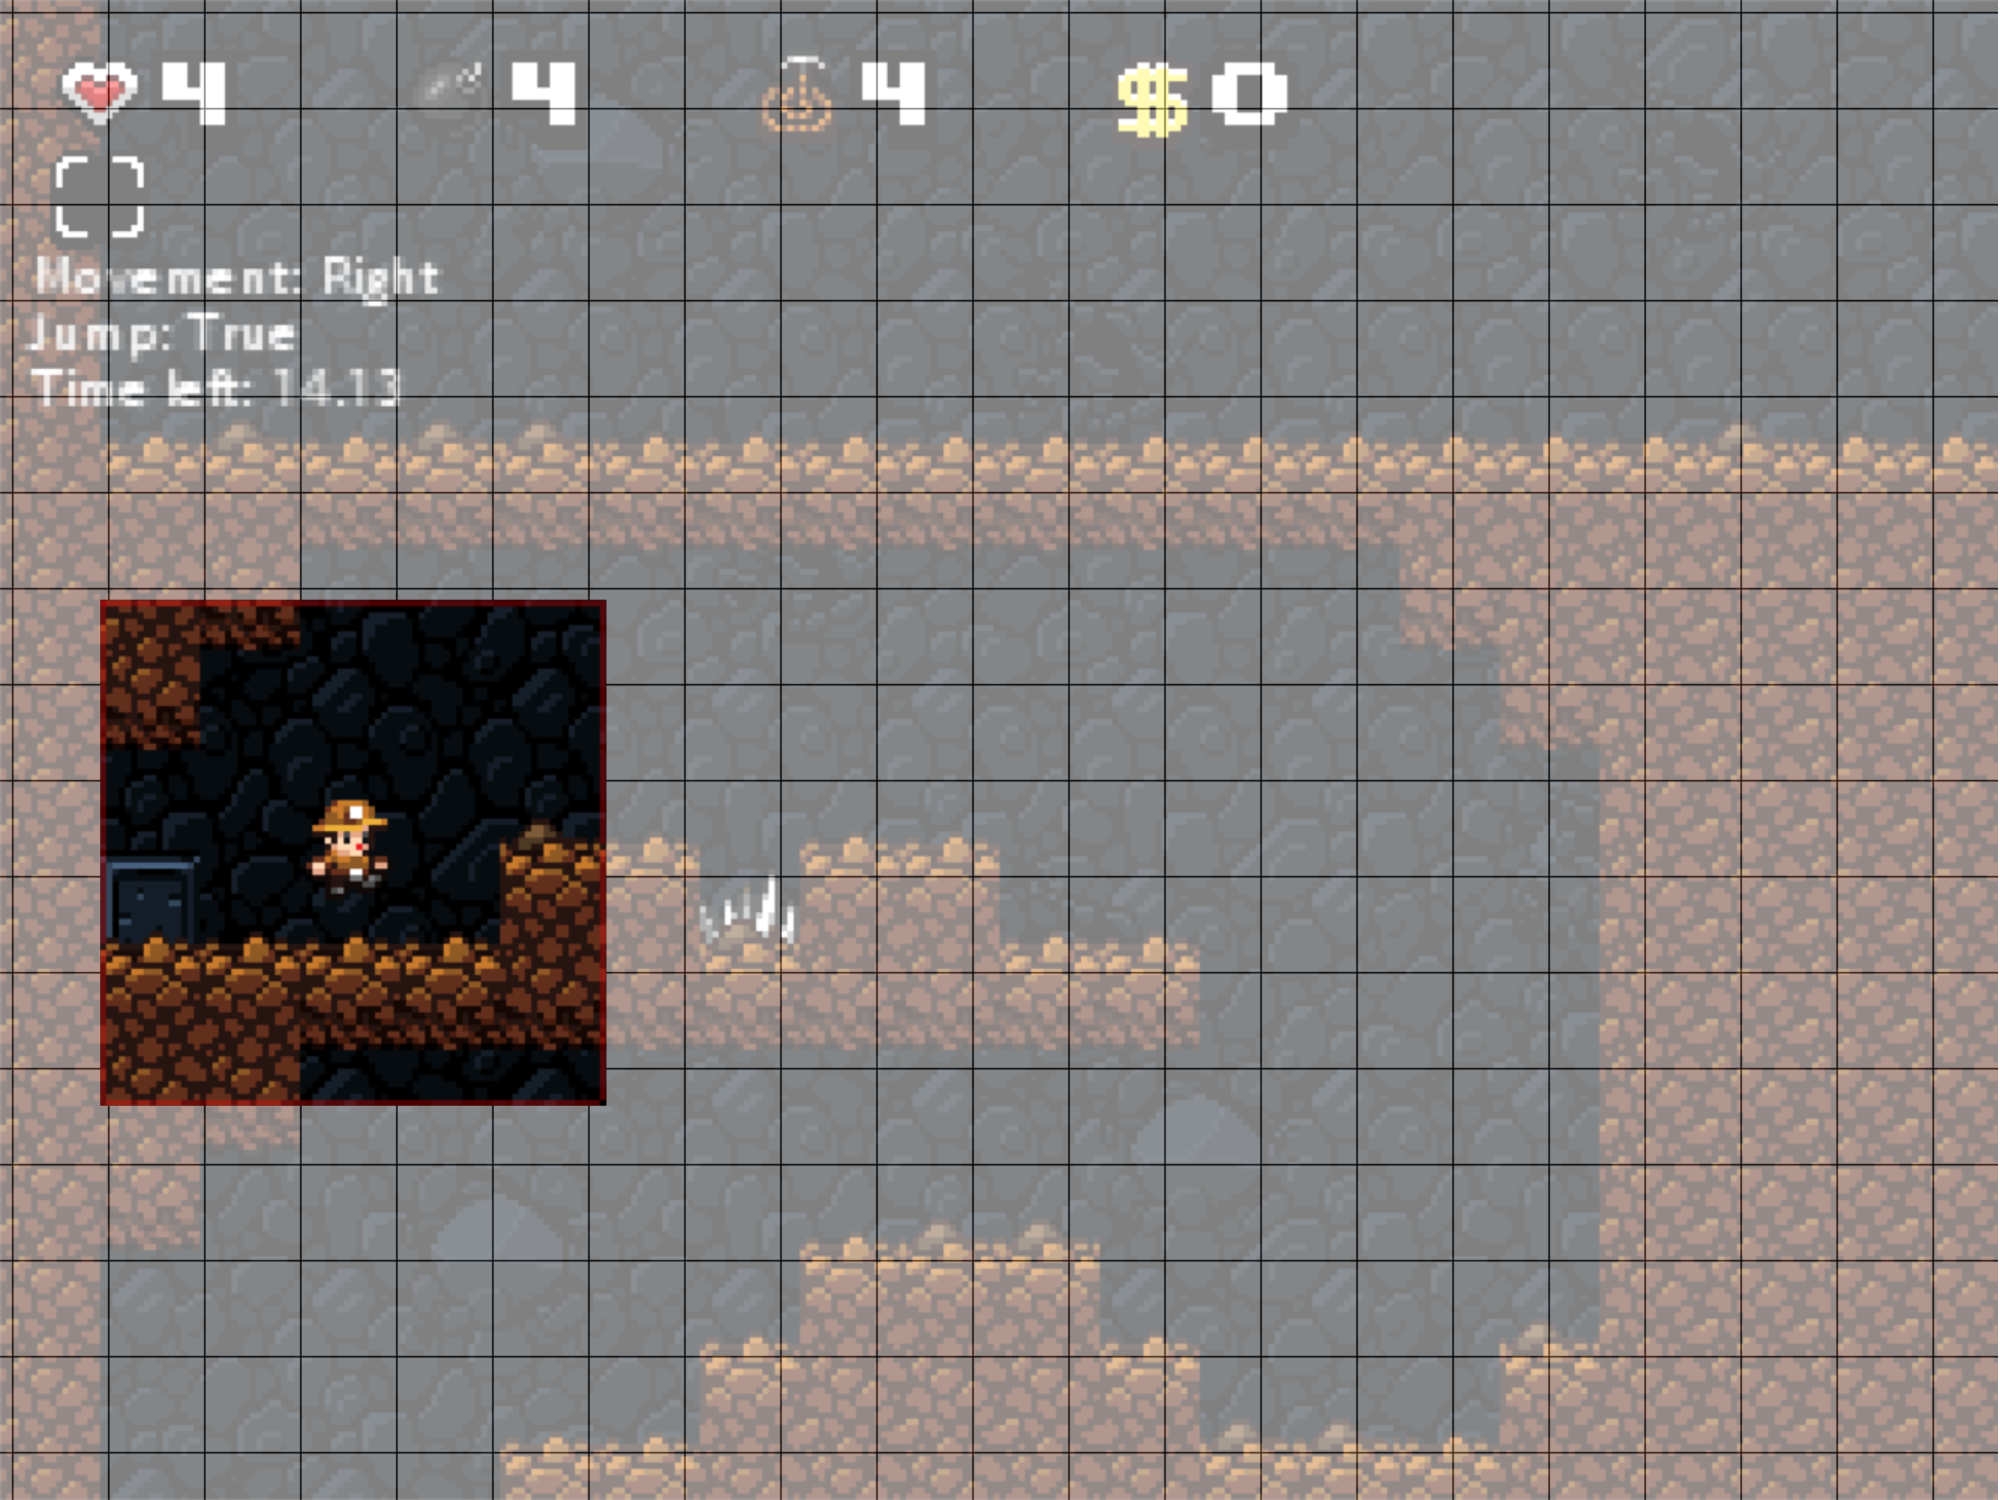
\includegraphics[width=.65\textwidth]{fig/spelunkbots-bot-vision.pdf}
\caption{\label{fig:vision-limitation}Exemplo da visão que um agente jogador de
\textit{Spelunky} tem enquanto está jogando.}
\end{figure}

\begin{figure}[H]
\centering
	\begin{subfigure}[b]{0.15\textwidth}
        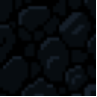
\includegraphics[width=\textwidth]{fig/spelunky-empty.pdf}
		\caption{Vazio.}
	\end{subfigure}
	\begin{subfigure}[b]{0.15\textwidth}
        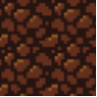
\includegraphics[width=\textwidth]{fig/spelunky-terrain.pdf}
		\caption{Terreno.}
	\end{subfigure}
	\begin{subfigure}[b]{0.15\textwidth}
        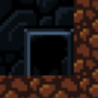
\includegraphics[width=\textwidth]{fig/spelunky-end-door.pdf}
		\caption{Saída.}
	\end{subfigure}
	\begin{subfigure}[b]{0.15\textwidth}
        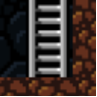
\includegraphics[width=\textwidth]{fig/spelunky-stair.pdf}
		\caption{Escada.}
	\end{subfigure}
	\begin{subfigure}[b]{0.15\textwidth}
        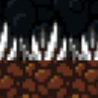
\includegraphics[width=\textwidth]{fig/spelunky-spike.pdf}
		\caption{Espinho}
	\end{subfigure}
	\caption{Exemplos dos nodos que o agente é capaz de enxergar.}
	\label{fig:vision-nodes}
\end{figure}

Não é possível identificar de antemão qual tamanho de visão será o mais adequado
para o agente sem realizar algum tipo de experimentação para realizar uma
validação empírica. Portanto, durante o treinamento dos agentes, realizaremos um
experimento para testar alguns tamanhos de área de visão (seção
\ref{section:experiment-vision}).


%----------
\section{\label{section:modelling-outputs}Ações do Agente}
A ferramenta \textit{SpelunkBots} permite que o agente envie comandos de ação
para o personagem (detalhado na Seção \ref{section:spelunkbots-commands}). Para
tal, o agente deve modificar uma série de variáveis que estão mapeadas para os
botões de ação. Em \textit{Spelunky}, o jogador é capaz de executar um grande
número de ações -- e combinações de ações -- a cada etapa de atualização do
jogo. Algumas delas são influenciadas por itens equipados ou o estado atual do
jogador (no ar, pendurado, etc.), o que significa que o agente deve estar
preparado para lidar com uma gama gigantesca de possibilidades de ações.

Considerar todas as ações disponíveis não é uma boa ideia por dois motivos.
Primeiramente, muitas destas ações não são necessárias para navegar pelo mapa, e
algumas podem inclusive, irônicamente, dificultar a navegação, como colocar
bombas ou cordas, pois criariam mais problemas do que resolveriam (rotas
adicionais, lidar com pontos de vida, etc.). Por fim, como mencionamos na seção
\ref{section:modelling-vision}, devido às limitações do \textit{SpelunkBots}, o
tamanho da rede neural pode influenciar na performance dos bots. Portanto, é
interessante eliminar a possibilidade de execução de todas as ações que não
trarão benefício para a navegação.

Assim, limitamos as ações que os agentes podem executar a \textbf{Movimentação}
(Esquerda e Direita) e \textbf{Pulo}. Caso algum dos cenários de teste
desenvolvidos requira ações adicionais, incluiremos conforme necessidade. Desta
forma, manteremos um controle ainda maior sobre cada caso de teste.


%----------
\section{\label{section:modelling-network}Configurações da Rede Neural}
Todos os agentes realizam a tomada de decisão de quais ações tomar baseados em
uma rede neural. Portanto, é importante detalhar como decidimos configurá-las
para execução. Esta configuração foi baseada em nosso levantamento de material
teórico, localizado no Capítulo \ref{chap:theory}. Existem duas partes
fundamentais de nossas redes neurais que devem ser inspecionadas: os
\textbf{neurônios} e a \textbf{topologia}.

Existem três pontos significativos de configuração dos neurônios da rede neural,
que são os \textbf{intervalos de pesos de conexões}, encarregados de informar
aos neurônios o quao importante é a informação, a \textbf{função de integração},
responsável por unificar os dados que estão entrando no neurônio, e a
\textbf{função de ativação}, cujo papel é processar o resultado da função de
integração. Como estamos utilizando uma biblioteca de \textit{NEAT}, estas
configurações estão pré-estabelecidas, e são as seguintes: o intervalo de
valores de pesos é entre $-8$ e $8$; a função de integração é uma simples
adição; a função de ativação é do tipo sigmóide, mais especificamente, a função
logística, que mantém os valores normalizados no intervalo $[0,1]$:

\begin{equation}
	\label{eq:neat-activation}
	f(x) = \frac{1}{1+e^{-k*m}}
\end{equation}

onde $e$ é o número de \textit{Euler} (2.71828), $k$ é a inclinatura da curva
(4.924273) e $m$ é o valor de soma atual dentro do neurônio.

As especificações de topologia inicial também são determinadas pelo
\textit{NEAT}, conforme vimos na seção \ref{section:neat}. Apear de possuirmos a
opção de incluir recorrência na rede, optamos por deixar a rede o mais simples
possível (sem realimentação), porque este processamento extra poderia levar a um
gargalo de execução, afetando a pontuação dos agentes devido a uma perda de
tempo. Na camada de entrada, colocamos um nodo de \textit{bias} e  fizemos a
conexão dos dados de visão recebidos pelo \textit{SpelunkBots}, conforme citado
na seção \ref{section:modelling-vision}. Ou seja, caso o tamanho do campo de
visão de um agente for de uma área de 5 por 5, a rede teria 25 nodos de visão e
1 nodo de \textit{bias}, totalizando em 26 nodos de entrada. A técnica
\textit{NEAT} também especifica que, inicialmente, não devem existir camadas
escondidas na rede, para que a evolução possa acontecer somente conforme
necessidade. Portanto, nossas redes neurais não possuem, inicialmente, nenhuma
camada escondida. Nas saídas da rede, fizemos o mapeamento, um para um, das
ações que desejamos executar (listadas na seção \ref{section:modelling-outputs}).
Ou seja, se um agente pode executar duas ações, existirão dois nodos de saída na
rede.

Durante o início do desenvolvimento deste trabalho, a ação de movimentação
estava separada em dois nodos, um para esquerda e outro para a direita. Contudo,
como desejávamos diminuir ao máximo o tamanho da rede para diminuir o
processamento necessário, decidimos unir estes dois nodos em um só. Caso o valor
de saída do nodo de movimentação esteja entre $[0,0.4]$, o agente ativará a ação
de caminhar para a esquerda. Se o valor estiver entre $(0.4,0.6)$, o agente não
executará nenhuma ação de movimentação (zona morta). Por fim, caso o valor
esteja entre $[0.6,1]$, o agente executará a ação de caminhar para a direita.

Na primeira etapa de execução, os neurônios da camada de entrada estão ligados,
todos para todos, com os neurônios da camada de saída. Portanto, para calcular o
número inicial de conexões da rede, basta utiliarmos a fórmula:

\begin{equation}
	\label{eq:network-connections}
	C = N_e * N_s
\end{equation}

onde $N_e$ é o número de neurônios na camada de entrada e $N_s$ corresponde ao
número de neurônios na camada de saída. Sem a modificação citada acima, um
neurônio de \textit{bias} e um tamanho de área de visão de 5 por 5, nossa rede
neural possuiria $78$ conexões.  Com esta pequena modificação, o número de
conexões cai para $52$. A diferença parece ser insignificante, mas este é apenas
o número de conexões na primeira etapa de execução. Conforme o algoritmo
executa, mais nodos e conexões surgirão, portanto diminuir o número de conexões
iniciais pode ter um impacto significante com o passar do tempo. A Figura
\ref{fig:modelling-network-example} ilustra uma configuração inicial de rede
neural utilizada neste trabalho.

\begin{figure}[H]
\centering
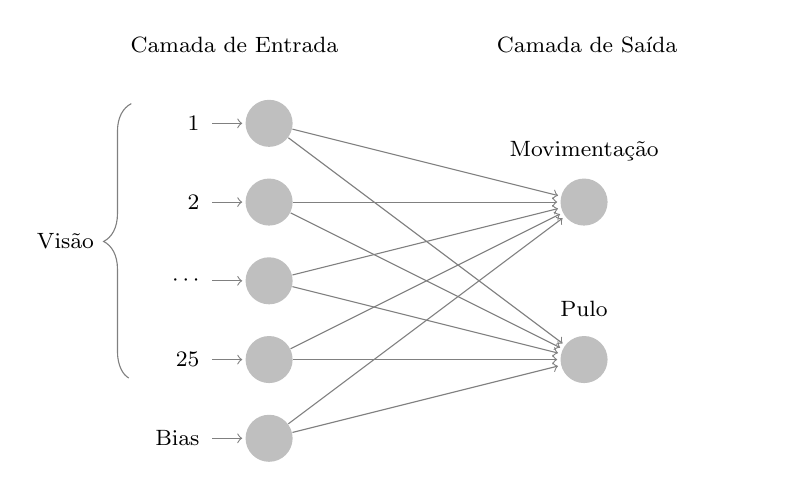
\begin{tikzpicture}[shorten >=1pt,->,draw=black!50, node distance=\layersep]
    \def\layersep{4cm}
    \tikzstyle{every node}=[font=\footnotesize]
    \tikzstyle{every pin edge}=[<-,shorten <=1pt]
    \tikzstyle{neuron}=[circle,fill=black!25,minimum size=17pt,inner sep=0pt]
    \tikzstyle{input neuron}=[neuron, fill=gray!50];
    \tikzstyle{output neuron}=[neuron, fill=gray!50];
    \tikzstyle{hidden neuron}=[neuron, fill=gray!50];
    \tikzstyle{annot} = [text width=10em]

    \node[input neuron, pin=left:1]        (I-0) at (0, 0)  {};
    \node[input neuron, pin=left:2]        (I-1) at (0, -1) {};
    \node[input neuron, pin=left:$\cdots$] (I-2) at (0, -2) {};
    \node[input neuron, pin=left:25]       (I-3) at (0, -3) {};
    \node[input neuron, pin=left:Bias]     (I-4) at (0, -4) {};

    \draw[decoration={brace,mirror,amplitude=10pt},decorate, style={-}]
      (-1.75,0.25) -- node[midway, left=10pt] {Visão} (-1.75, -3.25);

    \node at (\layersep, -0.35) {Movimentação};
    \node[hidden neuron] (O-0) at (\layersep, -1) {};
    \node at (\layersep, -2.35) {Pulo};
    \node[hidden neuron] (O-1) at (\layersep, -3) {};

    \foreach \source in {0,...,4}
        \foreach \dest in {0,...,1}
            \path (I-\source) edge (O-\dest);
    \node[annot] at (0, 1) {Camada de Entrada};
    \node[annot] at (4.65cm, 1) {Camada de Saída};
\end{tikzpicture}
\caption {\label{fig:modelling-network-example}Exemplo de configuração de rede
	neural inicial com campo de visão 5 por 5.}
\end{figure}

Conforme mencionado na seção \ref{section:modelling-outputs}, adicionaremos
neurônios na camada de saída conforme necessidade, ou seja, caso algum cenário
de teste exija do agente alguma ação a mais, esta ação será inserida na rede
inicial.


%----------
\section{\label{section:modelling-genetic}Configurações do Algoritmo Genético}
A técnica \textit{NEAT}, de acordo com a literatura explorada na seção
\ref{section:neat}, se baseia na neuroevolução para treinar as redes neurais
artificiais. Como ela evolui tanto os pesos das conexões quanto a topologia da
rede, as redes neurais são classificadas como \textit{TWEANNs}. O algoritmo
evolutivo do \textit{NEAT} é muito promissor pois resolve três problemas
extremamente comuns da neuroevolução: a permutação, a proteção da inovação e
população inicial. Listamos, a seguir, as características definidas como mais
importantes de um algoritmo genético, definido em
\ref{section:evolutionary-algorithms}, e como a técnica os resolve:

\begin{description}
	\item[Representação]
		A representação é feita de maneira direta, de acordo com a Figura
		\ref{fig:neat-encoding-example}.

	\item[Função de Aptidão]
		Esta função não é fornecida pelo \textit{NEAT} pois depende do domínio
		do problema. Portanto, deve ser disponibilizada por nós para o
		algoritmo. As descrições das funções de aptidão que desenvolvemos estão
		localizadas na seção \ref{section:modelling-fitness}.

	\item[População]
		O tamanho da população deve ser grande o suficiente para permitir que a
		especiação ocorra e que haja diferenciação genética suficiente entre os
		organismos. Contudo, devido à incapacidade de acelerar a execução do
		\textit{SpelunkBots}, o tamanho da população não pode ser muito elevado,
		pois se não nossos testes levariam tempo demais para concluir. Portanto,
		escolhemos um número de população de \textbf{100} organismos.

	\item[Seleção de Pais] A seleção de pais no \textit{NEAT} é feita de forma
		aleatória. Ou seja, a cada iteração, o algoritmo seleciona um ou dois
		pais para fazer mutações ou cruzamentos, respectivamente.

	\item[Variação] As probabilidades de realizar mutações e cruzamentos na
		biblioteca escolhida (detalhada na seção \ref{section:neat-details}) são
		definidas através de um arquivo externo que mapeia uma característica
		para uma probabilidade de acontecimento. As principais características
		que modificamos foram:
		\begin{itemize}
				\item força de mutação de pesos: $2.5$
				\item probabilidade de mutação de peso: $90\%$
				\item probabilidade de adição de nodo: $3\%$
				\item probabilidade de adição de conexão: $5\%$
				\item tamanho da população: $100$
		\end{itemize}

	\item[Seleção de Sobreviventes]
		A cada iteração, a geração anterior é substituida completamente por uma
		geração nova, baseada na mutação e cruzamento dos organismos anteriores.
		Para criar os novos organismos, o algoritmo organiza as espécies por
		ordem de maior aptidão e, então, distribui um pedaço da população para
		cada uma.

\end{description}

Também selecionamos os valores dos coeficientes de similaridade entre
organismos, integrantes da fórmula \ref{eq:neat-species}:

\begin{itemize}
	\item \textbf{$c_1$ (excess genes):} 1
	\item \textbf{$c_2$ (dijoint genes):} 1
	\item \textbf{$c_3$ (matching genes):} 0.4
\end{itemize}

O valor máximo estipulado para dois organismos pertencerem a mesma espécie,
calculado através da Equação \ref{eq:neat-species}, é de $\delta = 3$.

Para inicializar as redes neurais, o algoritmo conecta todos os neurônios da
camada de entrada com todos os neurônios da camada de saída e cada ligação
possui um peso inicial aleatório. A condição de parada do algoritmo varia de
acordo com o cenário de teste executado, mas sempre será estabelecido um número
máximo de iterações e um tempo máximo de teste.


%----------
\section{\label{section:modelling-fitness}Funções de Aptidão}
A tarefa de criar uma função de aptidão é uma das partes mais difíceis da
aplicação de um algoritmo genético para resolver um problema computacional. Isto
porque o desenvolvedor deve selecionar e experimentar com características do
domínio para encontrar parâmetros que mapeiem corretamente os requisitos que
deseja que seus agentes alcancem dentro do domínio. Se a função não mapear
eficientemente os objetivos desejados, é possível que o algoritmo genético tenha
dificuldades de convergir ou até mesmo convirja para uma solução inapropriada.

Poderiamos definir, por exemplo, uma função de aptidão de maneira extremamente
simplista: se o agente vencer, receberá um valor de aptidão de $1$; caso
contrário, receberá $0$. É possível que esta função funcione eventualmente mas,
dada a complexidade do cenário trabalhado, isto é extremamente improvável. Além
disso, somente o sucesso e o fracasso estão mapeados. Logo, não existe uma
maneira quantitativa de o algoritmo evolutivo identificar resultados
intermediários bons e ruins (retardando o aprendizado), além de ser impossível
identificar quais agentes, entre os bem-sucedidos, são mais eficientes.

Por conseguinte, devemos buscar características do domínio que auxiliem o
algoritmo evolutivo a acelerar o processo de aprendizado. Ao analisarmos o
domínio de navegação e as características de \textit{Spelunky}, identificamos
que nossas funções de aptidão deveriam se basear em duas características
fundamentais: \textbf{distância percorrida} e \textbf{tempo para conclusão}. O
raciocínio por trás da seleção destes parâmetros é simples: se o agente cobrir
uma quantidade maior de terreno, é provável que encontre, eventualmente, a
saída; paralelamente, quanto mais rápido o fizer, mais eficiente o agente será.

É interessante normalizar os valores obtidos de distância e tempo para que
possamos efetuar um balanceamento de importância destes parâmetros. Portanto,
devemos encontrar uma maneira de calculá-los fazendo com que fiquem dentro de
uma determinada região de valores. Um dos requisitos do algoritmo \textit{NEAT}
é que \textbf{os valores de aptidão devem ser positivos}, portanto optamos por
normalizá-los entre o intervalo $[0, 1]$.

\subsection{Distância Percorrida}
Ao iniciar um nível, o personagem é colocado na porta de entrada e deve navegar
pelo mapa e chegar na porta de saída. Um possível cálculo de distância
percorrida é a distância entre a posição final do jogador comparada com a
posição da porta de saída. Contudo, devido ao sistema de \textit{fog of war} do
\textit{SpelunkBots} (ilustrado na Figura \ref{fig:spelunkbots-fow}), não
sabemos qual é a localização exata da porta de saída, a não ser que a
visualizemos durante a execução. Além disso, caso nos baseássemos na distância
do jogador até a porta, nossos agentes obteriam uma vantagem significativa sobre
jogadores humanos, pois mesmo ao ser derrotado, é possível que um humano jamais
saiba a localização exata da porta de saída do mapa que acabou de tentar
superar. Portanto, utilizaremos como \textbf{valor base} a distância entre a
\textbf{posição final do jogador} e a \textbf{posição da porta de entrada}. Este
cálculo de distância se baseará na \textbf{Distância de Manhattan}:

\begin{equation}
	\label{eq:manhattan-distance}
	MD(p_1,p_2) = |p_1.x - p_2.x| + |p_1.y - p_2.y|
\end{equation}

onde $p_1$ e $p_2$ representam as coordenadas $(x,y)$ da porta de entrada e do
jogador, respectivamente. 

Para calcular o parâmetro de distância percorrida de forma normalizada, devemos
encontrar uma forma de estipular um valor máximo aproximado de distância que o
agente pode percorrer. Para tal, nos baseamos nas seguintes características
físicas que todo nível de \textit{Spelunky} apresenta:

\begin{itemize}
	\item os mapas sempre possuem um tamanho fixo de 42 por 34, mas o tamanho de
		área navegável é de 40 por 32 (existe uma borda indestrutível ao redor
		da região do mapa).
	\item o jogador sempre inicia no topo do mapa e a saída sempre se encontra
		na parte inferior do mapa.
\end{itemize}

No pior dos casos, a porta de entrada do mapa estaria localizada na posição
$(1,1)$ e a saída na posição $(40,32)$. Sabendo que o jogador sempre iniciará na
posição da porta de entrada do nível e utilizando a fórmula para distância de
Manhattan, obtemos $D_{max} = 70$, que corresponde ao máximo de distância que o
jogador deverá percorrer.

Agora, com os valores de base e máximo estipulados, é possível utilizar a
seguinte fórmula para calular a aptidão de distância percorrida, normalizada
entre o intervalo $[0,1]$:

\begin{equation}
	\label{eq:distance-fitness}
	D_{n}(p_{1},p_{2}) = MD(p_{1},p_{2}) / D_{max}
\end{equation}

onde $p_1$ e $p_2$ representam as coordenadas $(x,y)$ da porta de entrada e do
jogador, respectivamente. 

\subsection{Tempo para Conclusão}
A ferramenta \textit{SpelunkBots} nos permite estabelecer um tempo máximo de
teste para uma execução ($T_{max}$), bem como detectar o tempo total utilizado
pelo agente durante o teste ($T_{elapsed}$). Com estas duas informações em mãos,
é simples de calcular uma aptião de tempo normalizada entre o intervalo $[0,1]$
através da seguinte fórmula:

\begin{equation}
	\label{eq:time-fitness-wrong}
	T_{n} = (T_{max} - T_{elapsed}) / T_{max}
\end{equation}

Contudo, calcular desta forma a aptidão do parâmetro de tempo resultaria em uma
anomalia indesejada: todos os agentes, independente do resultado da execução,
seriam recompensados (ou penalizados) com uma função de aptidão de tempo igual.
Destacamos, a seguir, alguns dos resultados específicos que encontramos ao
experimentar com este cálculo simples:

\begin{itemize}
	\item Os agentes descobriram que deveriam se matar o mais rápido possível,
		pois assim gastariam pouco tempo durante o teste e sua aptidão de tempo
		seria elevada.

	\item Os agentes que estavam explorando ativamente quando o tempo se
		esgotava eram penalizados da mesma forma que os agentes que morriam, que
		ficavam ociosos e que perambulavam por uma pequena área (não obtendo
		nenhum progresso real).

	\item Todos os agentes que não fossem bem-sucedidos receberiam a mesma
		penalidade: o valor mínimo da função de aptidão de tempo ($0$). Isto
		retarda o processo de aprendizado dos agentes, pois eles só poderão
		depender do parâmetro de distância percorrida para detectar seu
		progresso.
\end{itemize}

Analisando mais à fundo estes resultados, fica claro que existe uma falha na
concepção da função de aptidão de tempo: ela não limita suficientemente o
agente. Na verdade, o agente está fazendo exatamente aquilo que a função de
aptidão de tempo o pede, como fica evidenciado no primeiro resultado citado.
Portanto, decidimos criar um conjunto de regras para a função de aptidão de
tempo, baseada no resultado final da execução:

\begin{description}
	\item[Vitória]
		O agente atingiu a porta de saída. Neste caso sua aptidão de tempo deve
		ser relativa a quanto tempo levou até atingir a porta de saída. Logo,
		utilizamos a fórmula padrão de aptidão de tempo, ilustrada na Equação
		\ref{eq:time-fitness-wrong}.

	\item[Exploração]
		O agente estava explorando ativamente quando o tempo se esgotou. É
		possível que, dado mais tempo, o agente seja capaz de ser bem-sucedido.
		Neste caso, o valor de aptidão de tempo do agente será $0.01$, ou $1\%$
		de $T_{max}$.

	\item[Ocioso]
		O agente estava ocioso por muito tempo. É extremamente provável que
		nunca mais voltasse a se mexer. Neste caso, o valor de aptidão de tempo
		do agente será $0.001$, ou $0.1\%$ de $T_{max}$.

	\item[Repetição de Estados]
		O agente estava explorando apenas uma pequena área do mapa, repetindo
		excessivamente posições que já havia visitado antes. É extremamente
		provável que permaneca desta forma até o fim da execução. Neste caso, o
		valor de aptidão de tempo do agente será $0.001$, ou $0.1\%$ de
		$T_{max}$.


	\item[Morte]
		O agente se matou em um espinho (única forma de se matar atualmente em
		nossos cenários de teste), o que, evidentemente, é um resultado ruim.
		Neste caso, o valor de aptidão de tempo do agente será $0.001$, ou
		$0.1\%$ de $T_{max}$.
\end{description}


\subsection{Fórmulas Escolhidas}
Com os parâmetros de aptidão selecionados, o próximo passo é identificar uma
forma de combiná-los em uma fórmula única de aptidão. Esta parte também é
experimentativa, portanto, escolhemos algumas fórmulas candidatas: \textbf{média
aritmética}, \textbf{média ponderada} e \textbf{média harmônica}. Optamos por
realizar uma média entre os valores porque, apesar de não ser um requisito,
queremos continuar com os valores de aptidão normalizados.

A média aritmética, representada pela Equação \ref{eq:fitness-mean}, é a forma
mais simples de combinarmos os dois parâmetros escolhidos, pois ambos terão a
mesma importância. É possível que o algoritmo evolutivo possua informações
suficientes através desta fórmula.

\begin{equation}
	\label{eq:fitness-mean}
	M_{a} = \frac{D_{n} + T_{n}}{2}
\end{equation}

Já a média aritmética ponderada, representada pela Equação
\ref{eq:fitness-weighted-mean}, busca combinar os parâmetros priorizando de
forma diferente cada parâmetro de aptidão.  Aqui, queremos enfatizar a
importância da navegação, portanto seu peso será maior que o do tempo
necessário. Os valores de peso devem ser entre 0 e 1 e sua soma deve resultar 1.
Os pesos selecionados para distância ($W_{d}$) e tempo ($W_{t}$) serão de
\textbf{0.6} e \textbf{0.4}, respectivamente.

\begin{equation}
	\label{eq:fitness-weighted-mean}
	M_{w} = W_{d}*D_{n} + W_{t}*T_{n}
\end{equation}

Por fim, a média harmônica, representada pela Equação
\ref{eq:fitness-harmonic-mean}, busca combinar os parâmetros enquanto tende a
diminuir o valor da média obtida caso a diferença entre os valores seja muito
elevada. Neste caso, queremos identificar se os melhores resultados de aptidão
ocorrem quando existe um balanceamento entre os parâmetros de distância e tempo.
Caso haja um desbalanceamento, a função tenderá a diminuir a aptidão total dos
agentes.

\begin{equation}
	\label{eq:fitness-harmonic-mean}
	M_{h} = \frac{2}{\frac{1}{D_{n}} + \frac{1}{T_{n}}}
\end{equation}

A escolha de como combinar valores de aptidão baseados em mais de um parâmetro
também é experimentativa. Por isso, executamos testes com todas as funções aqui
citadas para analisar os resultados obtidos com cada uma delas. Tais testes
estão localizados na seção \ref{section:fitness-experiment}.

\chapter{\label{chap:development}Desenvolvimento}

O objetivo desse capítulo é apresentar detalhes da implementação, baseados na
modelagem apresentada no Capítulo \ref{chap:modeling}. Na Seção
\ref{section:project-details} apresentamos a arquitetura do projeto, mostrando
como os componentes se relacionam de forma a possibilitar a execução dos
\textit{bots}. Na Seção \ref{section:modifications} apresentamos as
modificações que realizamos no projeto original e os porquês dessas
modificações. Na Seção \ref{section:neat-details} apresentamos detalhes da
implementação do algoritmo \textit{NEAT}. Na Seção \ref{section:analytics}
apresentamos como coletamos e analisamos os dados de nossas execuções.

\section{\label{section:project-details}Detalhamento do Projeto}
O primeiro passo para dar início ao desenvolvimento deste projeto é obter uma
cópia do projeto \textit{SpelunkBots}, hospedada no \textit{website} de
versionamento de código
\textit{GitHub}\footnote{https://github.com/GET-TUDA-CHOPPA/SpelunkBots}. O
\textit{framework} conta com o código modificado do \textit{Spelunky} e uma
distribuição do \textit{GameMaker Pro 8.0}, utilizada para compilar e gerar o
arquivo executável do jogo.

Conforme detalhado na seção \ref{section:spelunkbots}, o \textit{SpelunkBots}
disponibiliza duas opções de linguagem de programação para realizar o
desenvolvimento dos \textit{bots}: \textit{GML} ou C++. Portanto, a próxima
etapa do projeto é definir a linguagem de programação que vamos utilizar. Para
este projeto, escolhemos a linguagem de programação \textbf{C++}, tendo em vista
que o desenvolvimento utilizando a linguagem \textit{GML} é extremamente
limitado. Além disso, é possível encontrar na Internet algumas bibliotecas em
C++ que implementam a técnica
\textit{NEAT}\footnote{http://nn.cs.utexas.edu/?neat-c}. O uso de uma biblioteca
salva tempo de desenvolvimento e permite que o foco do trabalho seja somente no
desenvolvimento dos \textit{bots}, e não na arquitetura necessária para tal.

Sabendo que a técnica \textit{NEAT} requer que o \textit{bot} receba treinamento
através de diversas simulações do jogo, optamos pelo uso de um servidor
dedicado, pois este processo pode ser demorado e realizá-lo em uma máquina
doméstica -- que está muito mais sujeita a ser desligada acidentalmente ou
intencionalmente -- seria arriscado. O servidor em questão utiliza um sistema
operacional baseado em \textit{Linux}.  Contudo, \textit{Spelunky} foi
desenvolvido utilizando uma versão muito antiga do \textit{GameMaker} e a
compilação do código externo do \textit{SpelunkBots} ocorre através de um
projeto em \textit{Visual Studio}.  Estas ferramentas só podem ser executadas no
sistema operacional \textit{Windows}. Como nosso servidor é baseado em
\textit{Linux}, é necessário realizar algumas adaptações no processo de
compilação e execução. Assim, utilizaremos os \textit{softwares}
\textit{MinGW}\footnote{http://www.mingw.org} e
\textit{Wine}\footnote{https://winehq.org}, que nos permitirão, respectivamente,
realizar uma compilação cruzada\footnote{Um compilador cruzado, ou
	\textit{cross-compiler}, é uma ferramenta de compilação capaz de produzir
código executável em uma plataforma diferente da qual o compilador está sendo
executado.} do código C++ para da plataforma \textit{Linux} para a plataforma
\textit{Windows}, gerando uma \textit{DLL}, e executar programas da plataforma
\textit{Windows} dentro do sistema operacional \textit{Linux}.

O próximo passo é escolher a biblioteca de inteligência artificial da técnica
\textit{NEAT} e incluí-la no processo de compilação da \textit{DLL},
integrando-a ao projeto \textit{SpelunkBots}. Ao concluir este passo, as
configurações iniciais do projeto estarão finalizadas e daremos início ao
processo de modelagem e desenvolvimento dos \textit{bots}. O diagrama
\ref{fig:project-diagram} ilustra a relação entre os elementos de configuração
do projeto.

\begin{figure}[h]
\centering
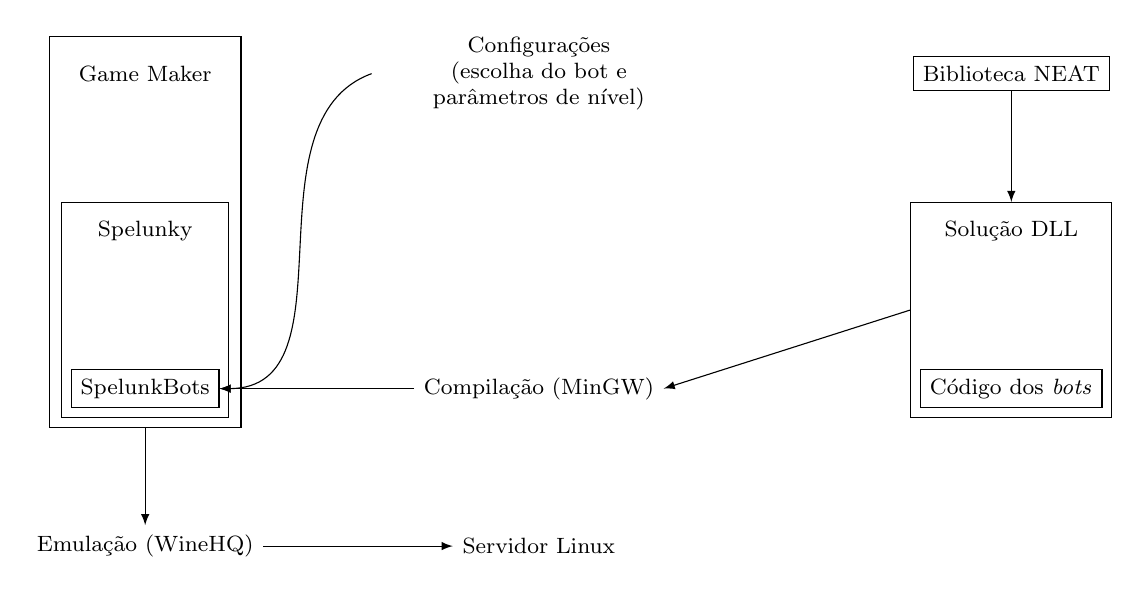
\begin{tikzpicture}
    \tikzstyle{every node}=[font=\footnotesize, text centered]
    \node (gmm) at (0, 0)  {Game Maker};
    \node (spl) at (0, -2) {Spelunky};
    \node[draw] (spb) at (0, -4) {SpelunkBots};

    \node[text width=4cm] (conf) at (5, 0)  {Configurações \\(escolha do bot e parâmetros de nível)};
    \node (comp) at (5, -4)  {Compilação (MinGW)};

    \node[draw] (neat) at (11, 0) {Biblioteca NEAT};

    \node (dll) at (11, -2) {Solução DLL};

    \node[draw] (bots) at (11, -4) {Código dos \textit{bots}};

    \node at (0, -6) (wine) {Emulação (WineHQ)};

    \node at (5, -6) (linux) {Servidor Linux};

    \node[draw, inner sep=.25cm, fit={(gmm) (spl) (spb)}] (g2) {};
    \node[draw, fit={(spl) (spb)}] {};

    \node[draw, fit={(dll) (bots)}] (g1) {};

    \draw[->, >=latex] (neat.south) -- (g1.north);

    \draw[->, >=latex] (g1.west) -- (comp.east);
    \draw[->, >=latex] (comp.west) -- (spb.east);

    \draw[->, >=latex, in=0, out=200] (conf.west) to (spb.east);

    \draw[->, >=latex] (g2.south) -- (wine.north);
    \draw[->, >=latex] (wine.east) -- (linux.west);
\end{tikzpicture}
\caption {Diagrama do projeto explicando a relação entre os componentes
necessários para o desenvolvimento dos \textit{bots}.
}
\label{fig:project-diagram}
\end{figure}

O \textit{framework} \textit{SpelunkBots} provê uma interface comum para o
desenvolvimento dos \textit{bots} em C++, chamada \textbf{\textit{IBot.h}}. Esta
interface é responsável por expor os métodos e variáveis que os \textit{bots}
utilizam para comunicar-se com o jogo. Portanto, qualquer código de \textit{bot}
desenvolvido deverá partir desta interface. Analisando o arquivo \textit{IBot.h}
é possível perceber que a interface obriga o desenvolvedor a implementar
\textbf{pelo menos} o método \textbf{\textit{Update}}, chamado em todas as
etapas de execução do \textit{bot} para receber informações e enviar comandos ao
jogo. Existem dois outros métodos que podem ser úteis ao desenvolvedor, mas que
não possuem obrigatoriedade de implementação: o \textbf{\textit{Reset}} e o
\textbf{\textit{NewLevel}}. O método \textit{Reset} é chamado no início de todas
as etapas de execução do \textit{bot} para reiniciar suas variáveis de controle.
Este método possui uma implementação padrão que reinicia apenas as variáveis
essenciais (esquerda, direita, pular e atacar). O método \textit{NewLevel} é
chamado toda vez que o \textit{bot} entra em um novo nível, e pode ser usado
para descartar informações do nível anterior sem que seja necessário reiniciar
todas as variáveis do \textit{bot}. Em sua implementação padrão, não executa
nada.

Uma implementação mínima de um \textit{bot} utilizando a interface
\textit{IBot.h} necessitaria, portanto, de dois arquivos: um arquivo
\textit{header}, que conterá as declarações dos métodos e variáveis a serem
utilizadas -- demonstrado no Algoritmo \ref{alg:project-example-bot-header} --,
e um arquivo de implementação -- demonstrado no Algoritmo
\ref{alg:project-example-bot-impl} --, que conterá a implementação das funções
descritas no arquivo \textit{header}.

\section{\label{section:modifications}Modificações do Código Original}

O código original do jogo conta com algumas características e limitações que
dificultavam o desenvolvimento desse trabalho. Contudo, temos acesso ao
código-fonte e somos capazes de modificá-lo. Assim, esta seção detalha as
modificações que fizemos, de forma a facilitar ou viabilizar o desenvolvimento.

\subsection{\textit{Scripts} de Compilação}

A escolha da linguagem \textit{C++} para a criação dos \textit{bots} requer a
compilação e geração de uma \textit{DLL} para que, posteriormente o
\textit{SpelunkBots} utilize-a. Este processo é feito em várias etapas.
Primeiro, compilamos as bibliotecas que utilizamos. Em seguida, compilamos o
código dos \textit{bots} e geramos a \textit{DLL}. Por fim, movemos a
\textit{DLL} para o local onde o \textit{SpelunkBots} será executado.

É necessário executar com sucesso todas as etapas de compilação para viabilizar
o desenvolvimento dos \textit{bots}. De forma a automatizar esse processo,
criamos um \textit{script} -- utilizando \textit{shell script} -- responsável
pelo processo de compilação e movimentação de arquivos.

\subsection{Pular Cena Inicial do Jogo}

O \textit{Spelunky} conta com uma cena inicial onde o jogador se desloca da
superfície para dentro de uma caverna. Esta caverna serve como menu principal do
jogo permitindo que o jogador escolhe entre fazer o tutorial do jogo, inciar sua
aventura, ver as maiores pontuações, entre outros. A Figura
\ref{fig:spelunky-introduction} apresenta a cena inicial e a caverna de menu
principal.

\begin{figure}[H]
\centering
	\begin{subfigure}[b]{0.4\textwidth}
		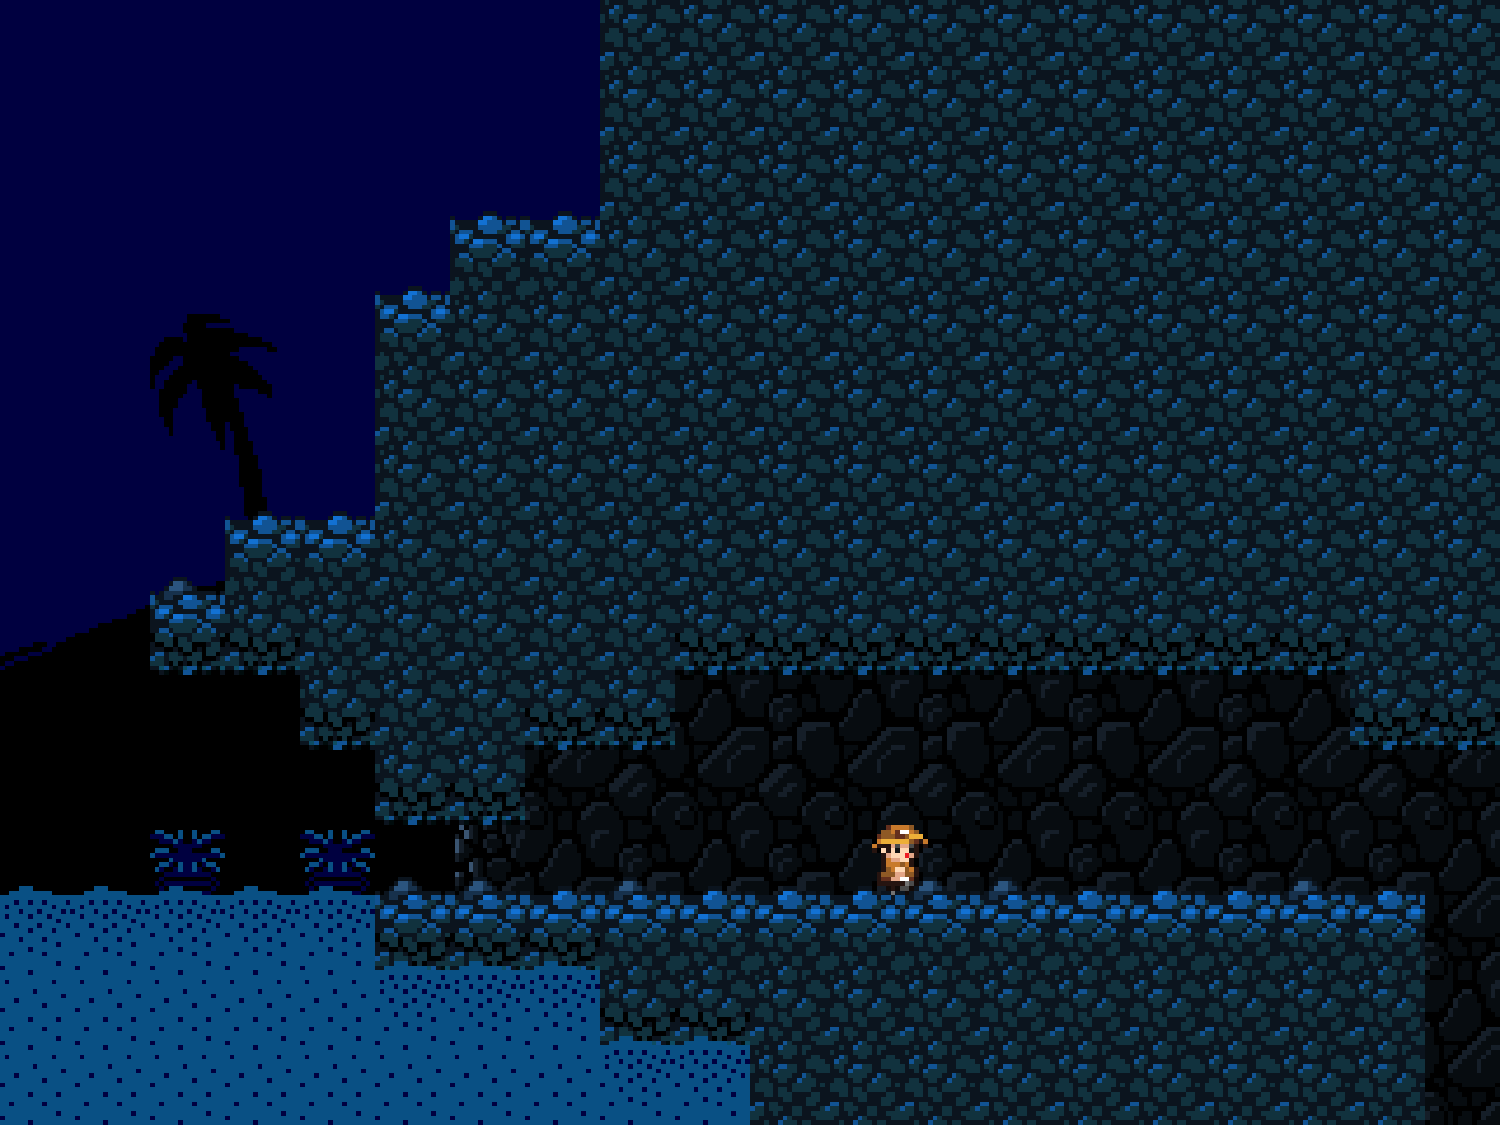
\includegraphics[width=\textwidth]{fig/spelunky-intro-screen.pdf}
		\caption{Entrada para a caverna inicial.}
		\label{fig:spelunky-intro-screen}
	\end{subfigure}
	\begin{subfigure}[b]{0.4\textwidth}
		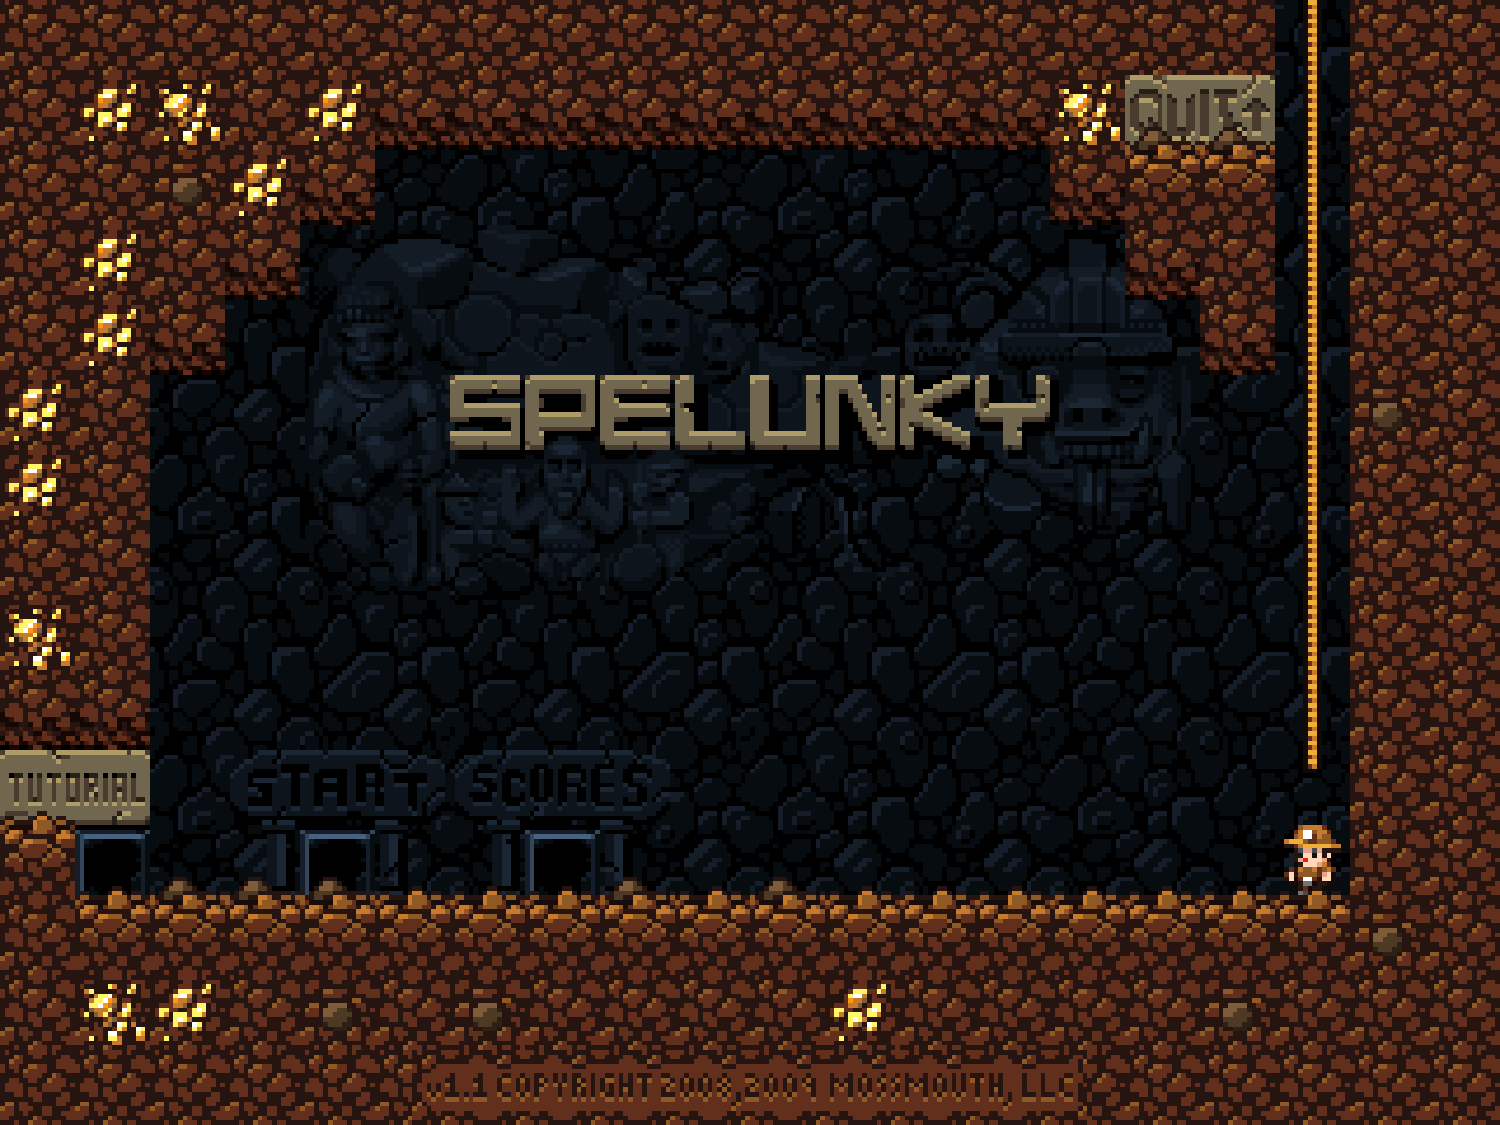
\includegraphics[width=\textwidth]{fig/spelunky-initial-screen.pdf}
		\caption{Caverna de escolha.}
		\label{fig:spelunky-initial-screen}
	\end{subfigure}

    \caption{Cena de introdução do jogo, onde o jogador se desloca da
    superfície para uma caverna com opções de interação.}
	\label{fig:spelunky-introduction}
\end{figure}

Estas cenas são apenas uma forma de introdução ao jogo, não contribuíndo para a
geração de resultados de execução. Logo, não necessitamos delas. Nossos
\textit{bots} devem ser levados diretamente até a opção de iniciar o jogo nos
mapas customizados que geramos.  Assim, utilizamos \textit{GameMaker} para
remover essas cenas. Portanto, ao executar o jogo, o \textit{bot} é levado
diretamente ao nível escolhido, executando imediatamante.

\subsection{Interrupção da Execução de Agentes não Promissores}

Devido às limitações apresentadas anteriormente na seção
\ref{section:spelunkbots-limitations}, é muito importante conseguirmos definir o
momento em que algum \textit{bot} esteja em um estado não promissor -- gastanto
tempo de execução --. Isso permite que interrompamos a execução, acelerando o
processo de treinamento.  Para isso, definimos dois critérios que nos concedem a
capacidade de identificar o momento em que um \textit{bot} está ocioso:

\begin{description}
	\item [Tempo parado] em alguns casos, o \textit{bot} pode escolher ficar
		parado. Porém, caso ele fique ocioso por muito tempo, é muito provável
		que nada de diferente ocorrerá até o fim da execução, dado que não
		existem elementos dinâmicos em nossos testes. Assim, quando
		identificamos que o \textit{bot} está parado há mais de \textbf{3
		segundos}, interrompemos sua execução, sinalizando sua ociosidade para
		aa função de aptidão.

	\item [Estados repetidos] o único elemento dinâmico em nossos testes é a
		posição do jogador no mapa. Portanto, podemos considerar que o estado do
		jogo depende das coordenadas do jogador. Caso o agente visite o mesmo
		estado mais de \textbf{10 vezes}, é possível identificar que ele está
		repetindo excessivamente suas ações e, possivelmente, não sairá de uma
		mesma região, não encontrando a porta de saída. Se este for o caso,
		interrompemos sua execução, sinalizando sua repetição de estados para a
		função de aptidão.
\end{description}

Com estes critérios de interrupção definidos, é necessário que tenhamos uma
forma de parar a execução do agente caso um dos cenários descritos acima ocorra.
Assim, implementamos uma função de \textbf{verificação de ociosidade} e uma
variável \textit{booleana} de suicídio no código do \textit{bot}. A cada ciclo
de execução do jogo, averiguamos se o \textit{bot} está parado e, caso esteja,
incrementamos um contador de tempo (este contador é zerado caso haja
movimentação). Após, incrementamos o contador que indica o número de vezes que o
\textit{bot} visitou a posição em que se encontra atualmente. Caso ele esteja
parado pelo determinado número de segundos ou tenha visitado o mesmo estado pelo
determinado número de vezes, sabemos que esse é um estado não promissor. Então,
ativamos a variável de suicídio cujo propósito é zerar o número de pontos de
vida do jogador, fazendo com que o \textit{bot} reinicie sua execução.

\subsection{Arquivo de Inicialização}

O processo de escolha das configurações para a execução do jogo requer
experimentação. É necessário combinar diferentes parâmetros e avaliar sua
execução, escolhendo então os parâmetros que produzem os melhores resultados.
No caso do \textit{SpelunkBots}, esta escolha está ligada diretamente à edição
do código do jogo no \textit{Game Maker}. Sempre que desejamos editar um
parâmetro de execução, abrimos o \textit{software}, realizamos a edição dos
valores, salvamos uma nova versão do jogo e então o executamos. Esse processo é
manual e custoso, dificultando a escolha dos melhores parâmetros para execução.  

Dessa forma, alteramos o código do \textit{SpelunkBots} para permitir a leitura
de um arquivo de inicialização
(\textit{.INI})\footnote{https://docs.yoyogames.com/source/dadiospice/002\_reference/file\%20handling/ini\%20files/index.html}.
Assim, podemos alterar os valores dos parâmetros de execução sem abrir o
\textit{GameMaker} para recompilar o código e gerar um novo arquivo executável.
Um arquivo \textit{.INI} é dividido em \textbf{seções} e cada seção possui
\textbf{pares} de chave para valor associado.

O Algoritmo \ref{alg:ini-file} apresenta um exemplo de arquivo de inicialização.
Utilizamos quatro seções distintas para diferenciar o propósito dos pares de
valor. \textit{\textbf{[Bot]}} representa as informações sobre o \textit{bot}
escolhido na execução. A entrada \textit{bot\_is\_cpp}, quando com o valor
\textbf{1}, indica que se trata de um \textit{bot} que foi escrito em
\textit{C++}, já a entrada \textit{bot\_cpp\_num} idica qual \textit{bot} será
executado.  A seção \textit{\textbf{[Test]}} informa dados relativos ao teste
que será realizado. O tipo de mapa é informado pela entrada \textit{test\_type}.
O parâmetro \textit{test\_rank} indica ao \textit{SpelunkBots} como classificar
a execução dos \textit{bots}. Podemos controlar o número \textbf{máximo} de
execuções pelo valor de \textit{test\_num}. Também é possível limitar o tempo de
vida de um \textit{bot} pelo parâmetro \textit{test\_time}, que é indicado em
segundos.  É possível especificar os níveis que queremos utilizar para testar os
agentes através da seção \textit{\textbf{[Levels]}}. Primeiro, indicamos a
quantidade de níveis pelo valor de \textit{level\_num}. Após, para cada nível,
indicamos o seu nome em uma propriedade específica. No caso do primeiro, usamos
a propriedade \textit{level0}, para o segundo, \textit{level1}, e assim para
todos eles.  Por fim, temos a seção \textit{\textbf{[FAMW]}}, que parametriza a
exibição de informações de depuração durante a execução do jogo.  O valor de
\textit{vision\_debug} indica se deverá ser exibida na tela uma janela da visão
do \textit{bot}, com o tamanho informado por \textit{vision\_size}.

\begin{algorithm}[H]
\lstinputlisting[style=customC++]{code/spelunkbots.ini}
	\caption[Exemplo de um arquivo de inicialização \textit{.INI}.]
{\label{alg:ini-file}Arquivo de inicialização de exemplo.}
\end{algorithm}

\subsection{\label{sub:virtual-display}Execução com Display Virtual}

Como vimos anteriormente, na seção \ref{section:spelunkbots-limitations}, não é
possível executar o jogo sem janela gráfica. Isto é um problema, pois o servidor
\textit{Linux} que utilizamos para a execução dos testes não possui nenhuma
interface gráfica.  Porém, é possível superar esta limitação através da
utilização de um \textit{display} virtual, onde simulamos uma interface gráfica
semelhante a uma real. Nesse caso, utilizamos o \textit{software}
\textit{XVFB}\footnote{https://www.x.org/archive/X11R7.6/doc/man/man1/Xvfb.1.xhtml},
criando então uma interface gráfica que recebe a execução do jogo. O uso de uma
interface gráfica virtual também nos permitiu realizar conexões remotas para o
servidor, concedendo-nos a capacidade de acompanhar o processo de treinamento em
tempo real.

\subsection{\label{sub:spelunkbots-gui}Interface de Acompanhamento do
SpelunkBots}

O \textit{SpelunkBots} conta com uma interface de acompanhamento da execução do
jogo. Além de possibilitar ver o personagem explorando a caverna, ela também
mostra alguns controles específicos do \textit{SpelunkyBots}, tais como os
botões que o jogador está apertando, além de algumas informações de direção.

Embora essa interface contenha muitas informações, muitas delas não são
relevantes no nosso caso. Além disso, implementamos alguns controles para o
jogo -- tal como o tempo máximo de execução -- que são interessantes de
acompanharmos. Portanto, modificamos essa tela de acompanhamento, deixando
apenas as informações que consideramos relevantes. Nesse caso, a direção para
onde o jogador está se movimentando e se ele está apertando o botão de pular.
Além disso, também queremos saber o tempo restante de execução. Assim, criamos
um contador que inicia com o tempo máximo estipulado vai sendo decrementado ao
longo do tempo. Também adicionamos um quadrado vermelho em volta do jogador,
indicando o campo de visão dele. A Figura \ref{fig:spelunkbots-gui} compara a
interface antes e depois das modificações.

\begin{figure}[H]
\centering
	\begin{subfigure}[b]{0.4\textwidth}
		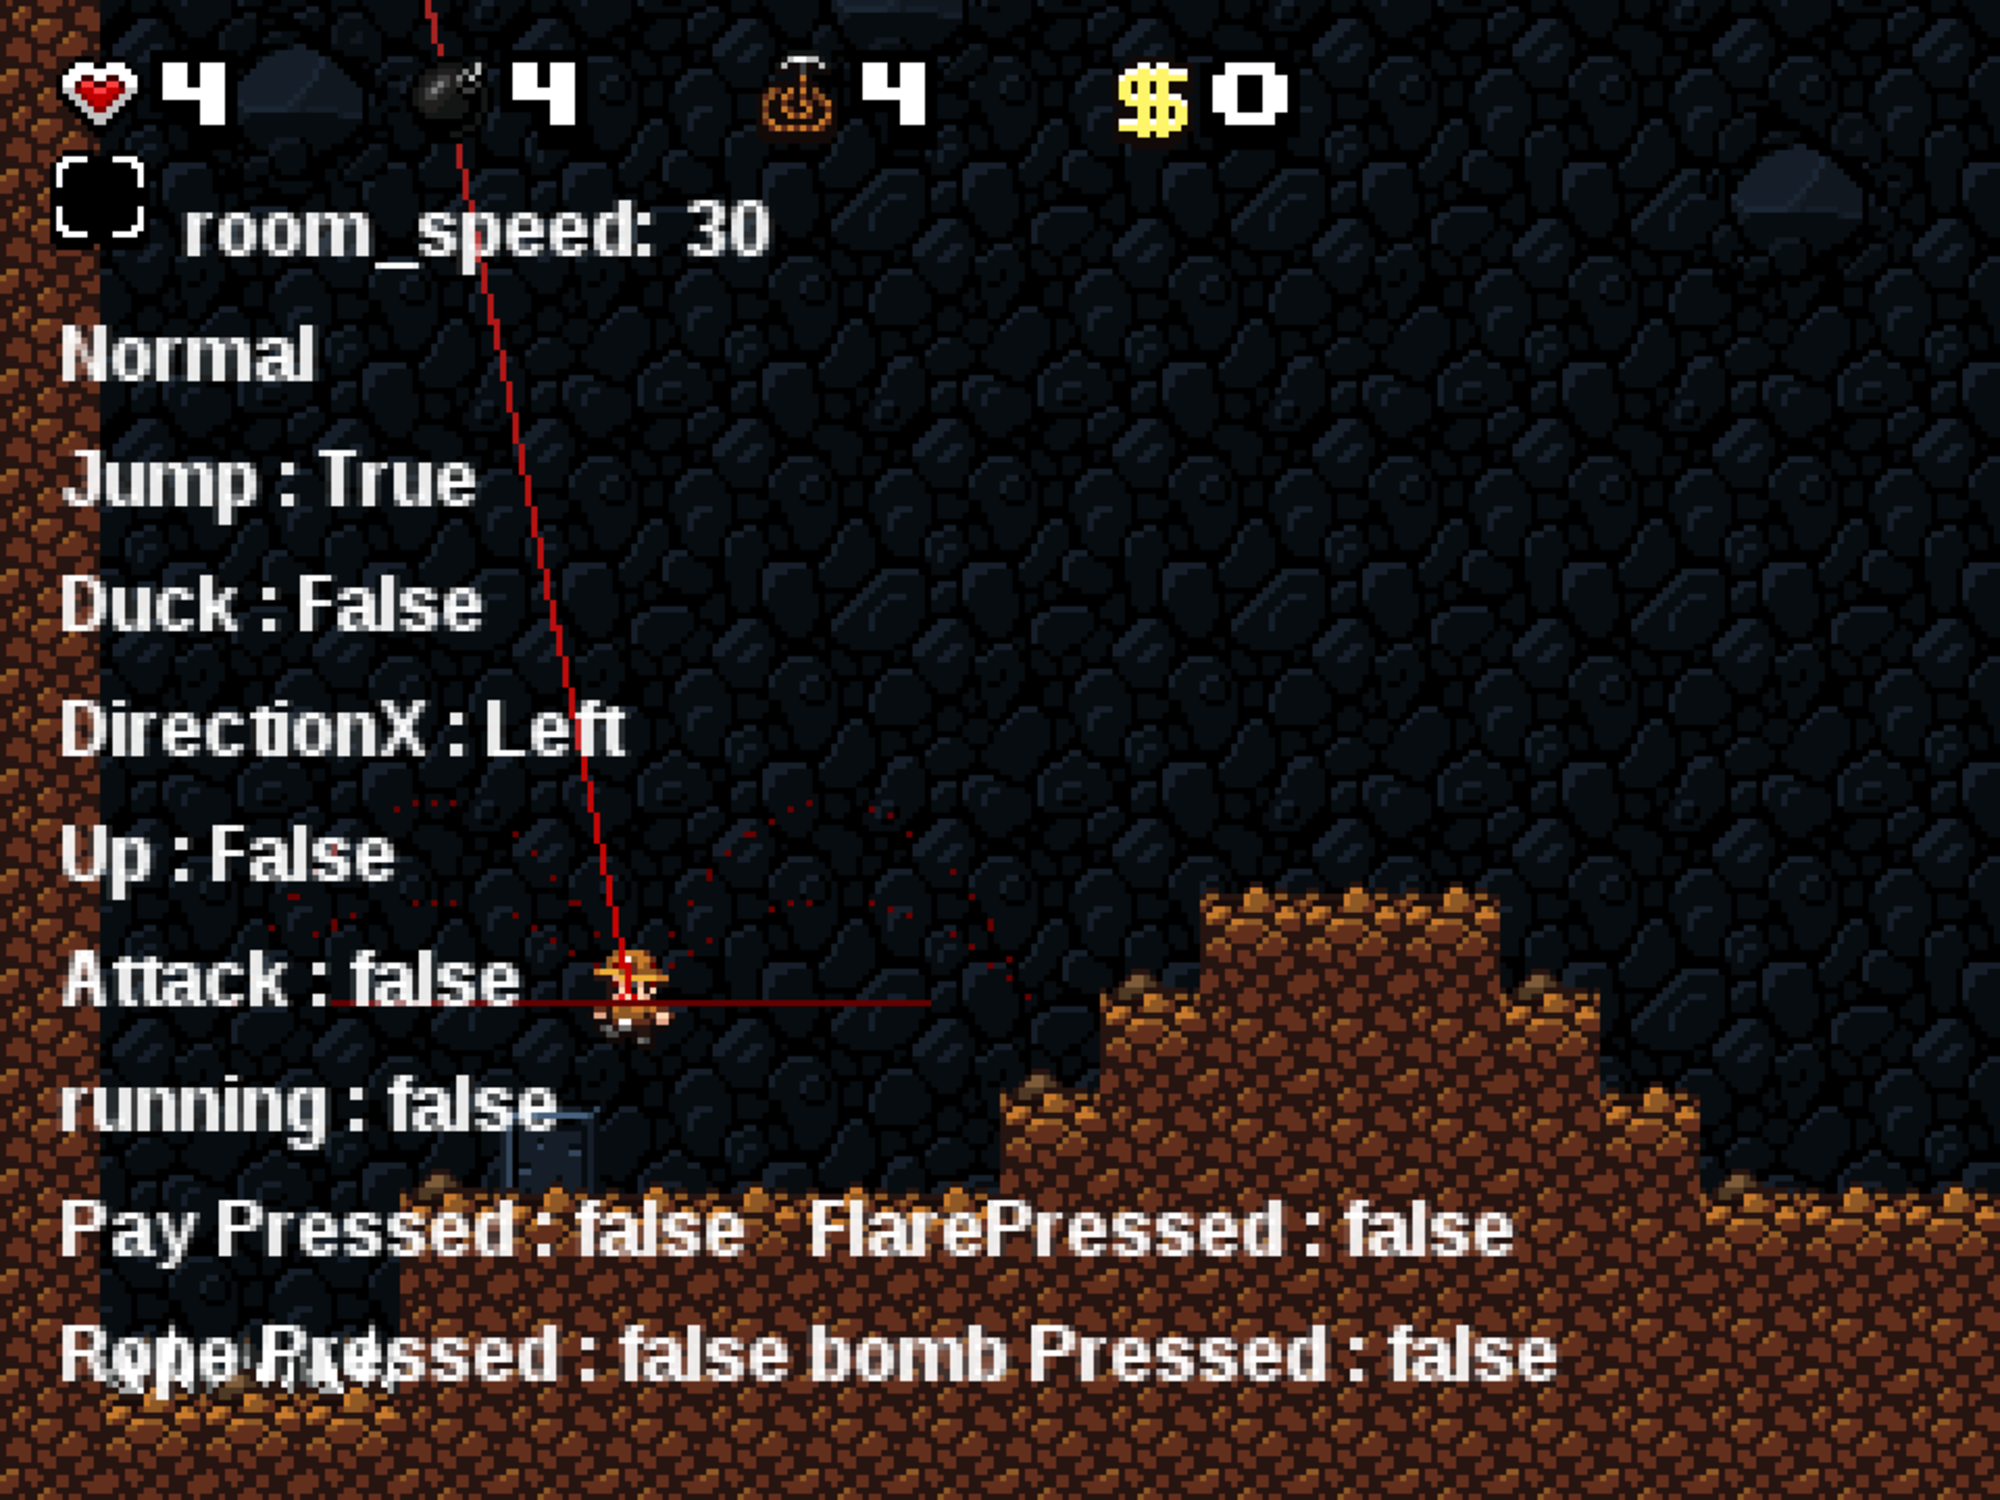
\includegraphics[width=\textwidth]{fig/spelunkbots-gui-before.pdf}
        \caption{Interface do \textit{SpelunkBots} antes das modificações realizadas.}
		\label{fig:spelunkbots-gui-before}
	\end{subfigure}
	\begin{subfigure}[b]{0.4\textwidth}
		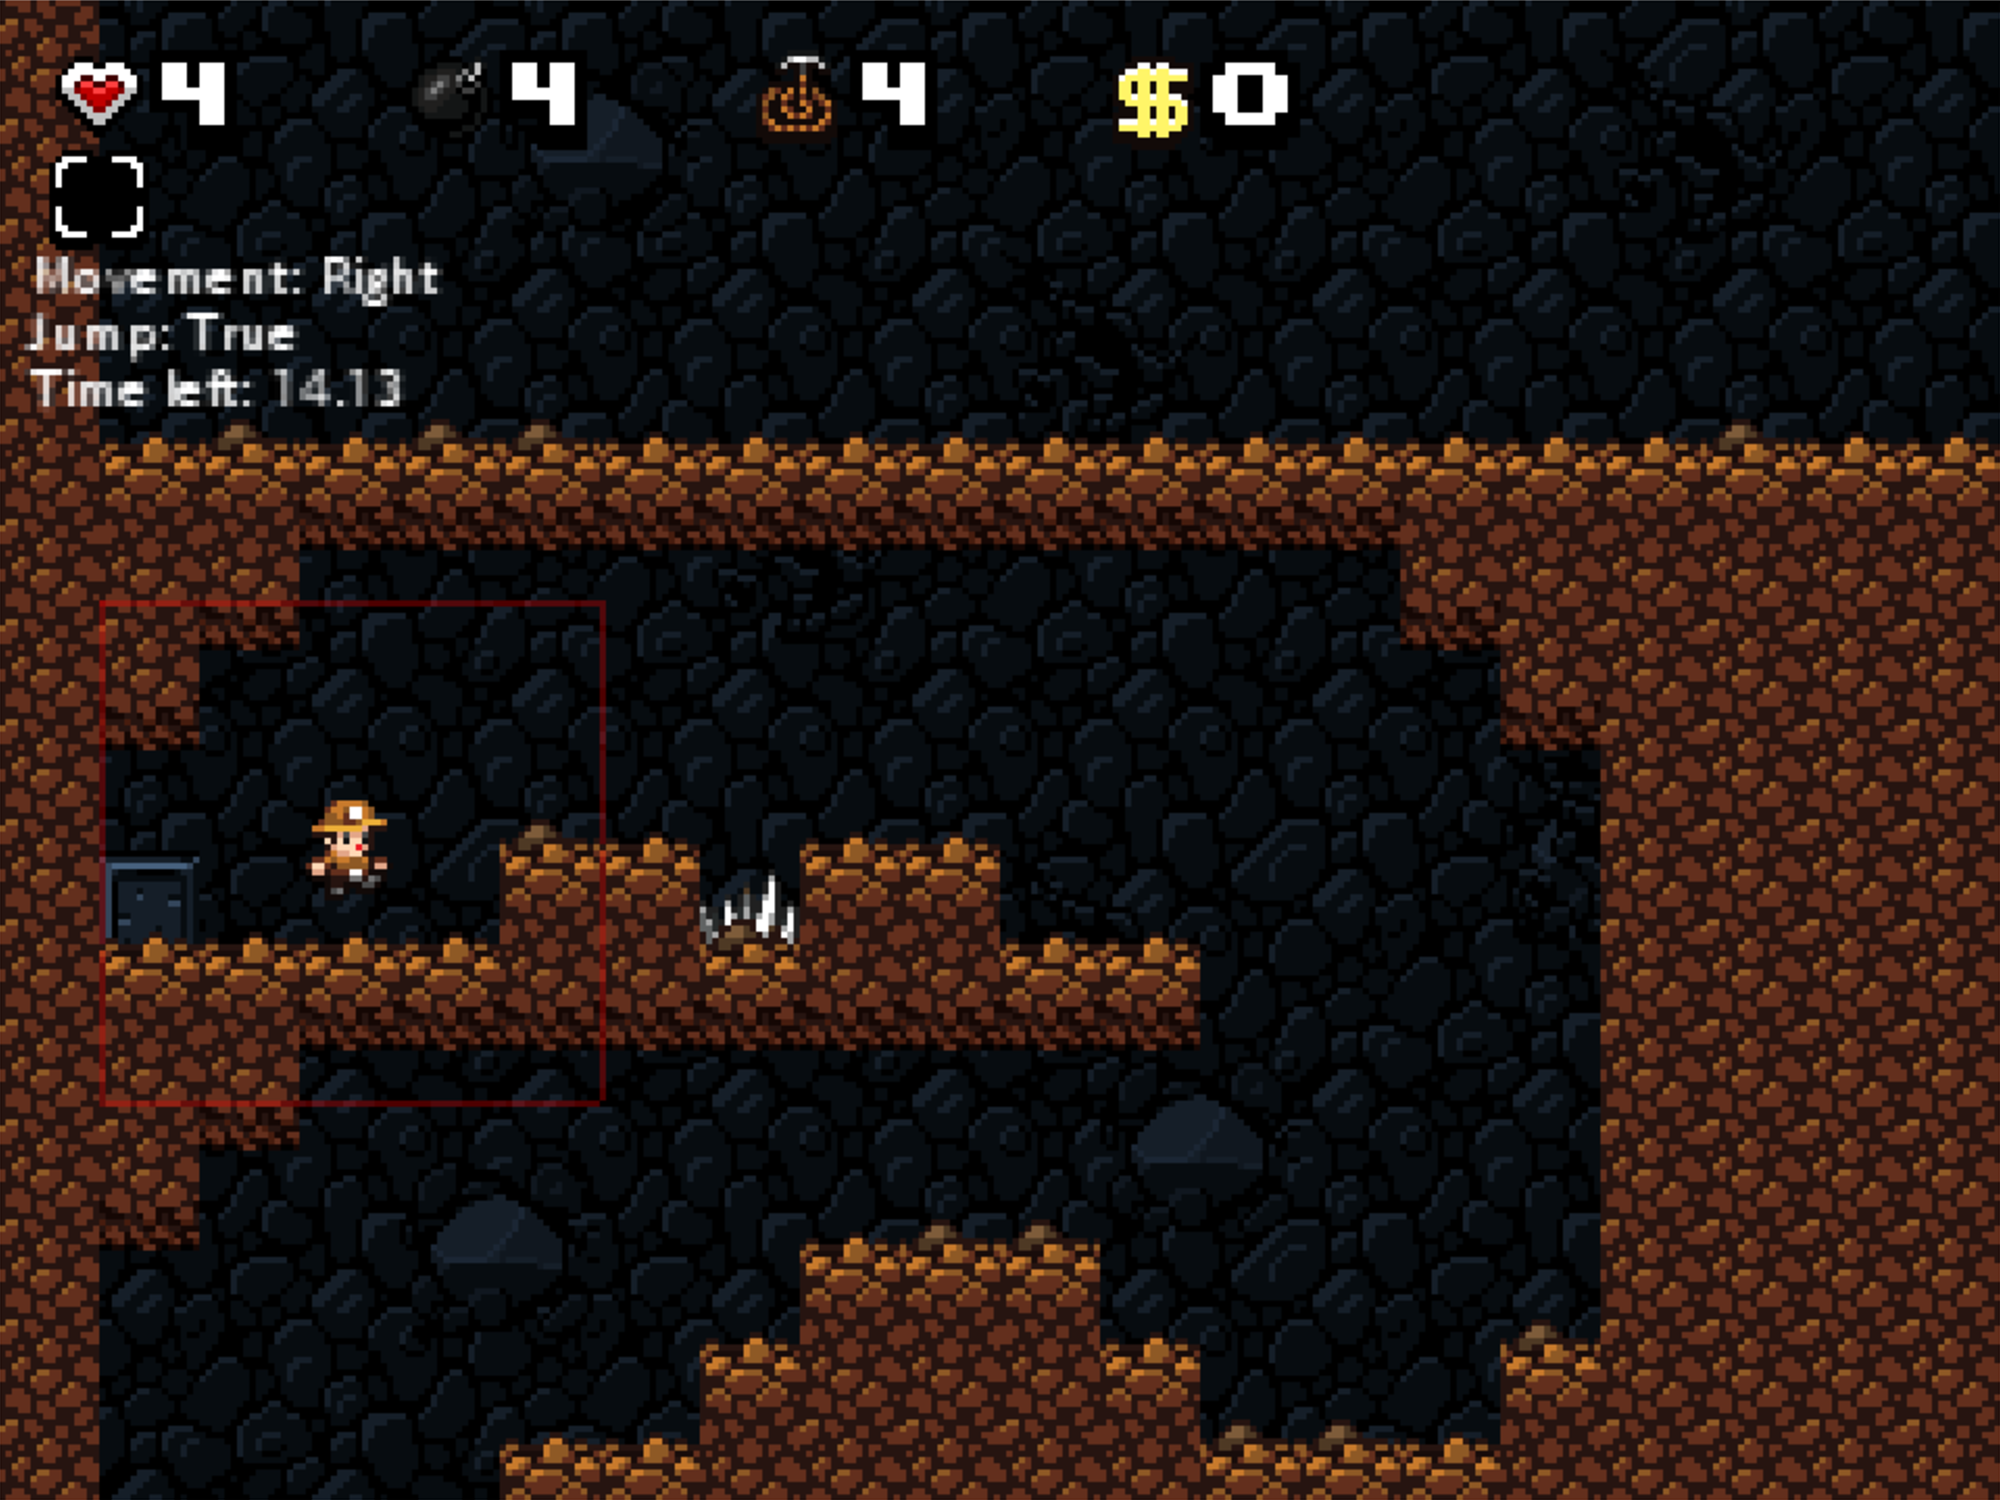
\includegraphics[width=\textwidth]{fig/spelunkbots-gui-after.pdf}
        \caption{Interface do \textit{SpelunkBots} após as modificações realizadas.}
		\label{fig:spelunkbots-gui-after}
	\end{subfigure}

    \caption{Comparação entre a interface do \textit{SpelunkBots} antes e
    depois das modificações realizadas.}
	\label{fig:spelunkbots-gui}
\end{figure}

\section{\label{section:neat-details}Implementação do NEAT}
Com o objetivo de poupar tempo na parte do desenvolvimento, optamos por utilizar
a biblioteca que implementa o algoritmo \textit{NEAT} disponibilizada pelo autor
da técnica\footnote{http://nn.cs.utexas.edu/?neat-c}. Antes de executar qualquer
treinamento, é necessário entender como configurar os parâmetros de execução da
biblioteca:

\begin{description}
	\item[Valor de Semente]
		A biblioteca utiliza um gerador de números pseudo-aleatórios para
		realizar a decisão de eventos randômicos como, por exemplo, decidir se
		vai mutacionar ou cruzar organismos, selecionar pais para cruzamento,
		entre outros. Portanto, é necessário abastecer este gerador com um valor
		de semente.

	\item[Configurações de Mutação]
		O desenvolvedor deve fornecer um arquivo de texto para a biblioteca com
		as configurações de mutação que deseja utilizar. O Algoritmo
		\ref{alg:neat-parameters-example}, localizado dentro do Apêndice
		\ref{appendix:neat-configs}, possui um exemplo de arquivo de
		configuração de valores de mutação.

	\item[Rede Neural Inicial]
		Outro requisito da biblioteca é que o desenvolvedor forneça um arquivo
		de texto contendo uma configuração de rede neural artificial. A
		biblioteca irá se basear neste arquivo para criar as redes neurais dos
		organismos pertencentes à população inicial. O Algoritmo
		\ref{alg:neat-network-example}, localizado dentro do Apêndice
		\ref{appendix:neat-configs}, possui um  exemplo de arquivo de
		configuração de rede neural inicial.
\end{description}

Para tentar garantir a reprodutibilidade de nossos testes, utilizamos a mesma
semente para popular o gerador de números pseudo-aleatórios em todas as
execuções: \textbf{12345}. Com estes parâmetros iniciais, a biblioteca é capaz
de gerar uma população inicial que respeite as estrutura de rede neural inicial
e evoluí-la de acordo com as configurações de mutação desejadas. Como o arquivo
de rede neural inicial é trabalhoso de se elaborar, desenvolvemos um programa em
C++ que gera automaticamente um arquivo de rede inicial dadas as especificações
desejadas\footnote{https://github.com/famw/neat-startgene-generator}.

Simplificando, o laço de execução do programa do agente, depois do carregamento
dos parâmetros de configuração, ocorre da seguinte maneira: primeiro, coletamos
as informações do jogo utilizando o \textit{SpelunkBots}. Em seguida, carregamos
estas informações nas entradas da rede neural do agente. Após, utilizamos a
função de ativação da rede neural para realizar o processamento dos dados.
Então, coletamos os valores dos neurônios da camada de saída da rede e
selecionamos, de acordo com os valores, quais ações o agente deseja executar.
Por fim, enviamos os comandos de ação ao \textit{SpelunkBots}, que executa-os
para nós.


\section{\label{section:analytics}Análise dos Dados}

A biblioteca de \textit{NEAT} escolhida gera uma série de informações dos
organismos ao fim de cada geração, como valor de aptidão, espécie do organismo,
identificação se o organismo foi vencedor ou não, entre outras. Estas
informações são extremamente úteis, pois podemos utilizá-las para realizar uma
análise do desempenho dos agentes, gerando gráficos ou tabelas com compilados de
informações. O Algoritmo \ref{alg:neat-output-example} mostra um exemplo deste
arquivo de texto para uma geração durante o treinamento.

\begin{algorithm}[H]
\lstinputlisting[style=customC++]{code/gen_example.pop}
\caption[Exemplo de arquivo de execução de um \textit{bot}.]
{\label{alg:neat-output-example}Exemplo de arquivo de execução de um
    \textit{bot}.}
\end{algorithm}

Logo, o próximo passo para analisar os dados foi escolher \textbf{o que queremos
analisar}. Decidimos que o mais interessante é analisarmos o \textbf{número de
organismos vencedores ao longo das gerações} e o \textbf{valor da função de
aptidão ao longo das gerações}. Em seguida, escolhemos que ferramenta iríamos
utilizar a fim de gerar visualizações mais intuitivas para estes dados
coletados. Como as nossas comparações são representadas por um valor -- ou o
número de vencedores, ou um valor de aptidão -- em função de um número gerações,
utilizamos uma \textbf{representação gráfica} que permite analisar esses
valores. Portanto, escolhemos o
\textit{gnuplot}\footnote{http://gnuplot.sourceforge.net/} para essa tarefa.

Contudo, essas informações ficam guardadas em um arquivo de texto não tratado,
ou seja, não é possível utilizar a saída gerada diretamente em algum
\textit{software} que permite a análise desses dados. Portanto, necessitávamos
de ferramentas para realizar um tratamento destes arquivos crús.  Para tal,
escolhemos as ferramentas
\textit{sed}\footnote{https://www.gnu.org/software/sed/} e
\textit{awk}\footnote{https://www.gnu.org/software/gawk/} em conjunto com
\textit{scripts}\footnote{https://github.com/famw/analytics} feitos em
\textit{bash}\footnote{https://www.gnu.org/software/bash/bash.html} para extraír
os dados e gerá-los em um formato interpretável pelo \textit{gnuplot}.

\chapter{\label{chap:scenarios}Cenários para Execução}

\todoin[caption={Melhorias nos cenários para execução}] {
    Para cada um dos cenários, adicionar o \textbf{critério de parada
    escolhido}.
}

\textit{Spelunky} é um jogo cheio de desafios para seus jogadores, sendo
possível realizar muitas ações do início ao fim de um nível. Através do
capítulo \ref{chap:spelunky}, podemos ter mais detalhes de muitos cenários
interessantes para este trabalho. Com isso, escolhemos alguns desafios que
julgamos interessantes para um agente inteligente que seja capaz de jogar
\textit{Spelunky}, explorando alguns cenários que serão encontrados em muitos
dos níveis do jogo.

\section{Cenários Convencionais}

O principal desafio do \textit{Spelunky} é fazer com que o jogador chegue até
o final do nível a partir da sua porta de entrada. Enquanto escapa de
obstáculos -- tais como inimigos e espinhos --, o jogador deve deslocar-se
horizontalmente e verticalmente entre o nível, buscando chegar até a porta de
saída. Visando explorar esse deslocamento, elaboramos alguns cenários
convencionais, categorizados por seu nível de dificuldade.

O nível \textbf{fácil} explora o deslocamento \textbf{horizontal}, em conjunto
com a necessidade de \textit{saltar} sobre espinhos e blocos. A figura
\ref{fig:level1} demonstra o nível fácil, onde o jogador parte da porta de
entrada -- localizada na esquerda --, devendo saltar sobre alguns blocos, pular
sobre alguns espinhos e chegar até a porta de saída. Esse nível é interessante
pois, além de explorar deslocamento e saltos, também conta com espinhos nas
extremidades -- à esquerda da entrada e à direita da saída --, o que faz com
que o jogador tenha que evitar entrar em contato com essas áreas.

Como este é um nível pouco desafiador, estabelecemos como \textbf{critério de
parada} para este nível duas condições:

\begin{description}
    \item [Número de execuções] no máximo \textbf{10000} execuções.
    \item [Tempo máximo de execução] no máximo \textbf{10 segundos} executando.
\end{description}

\begin{figure}[H]
\centering
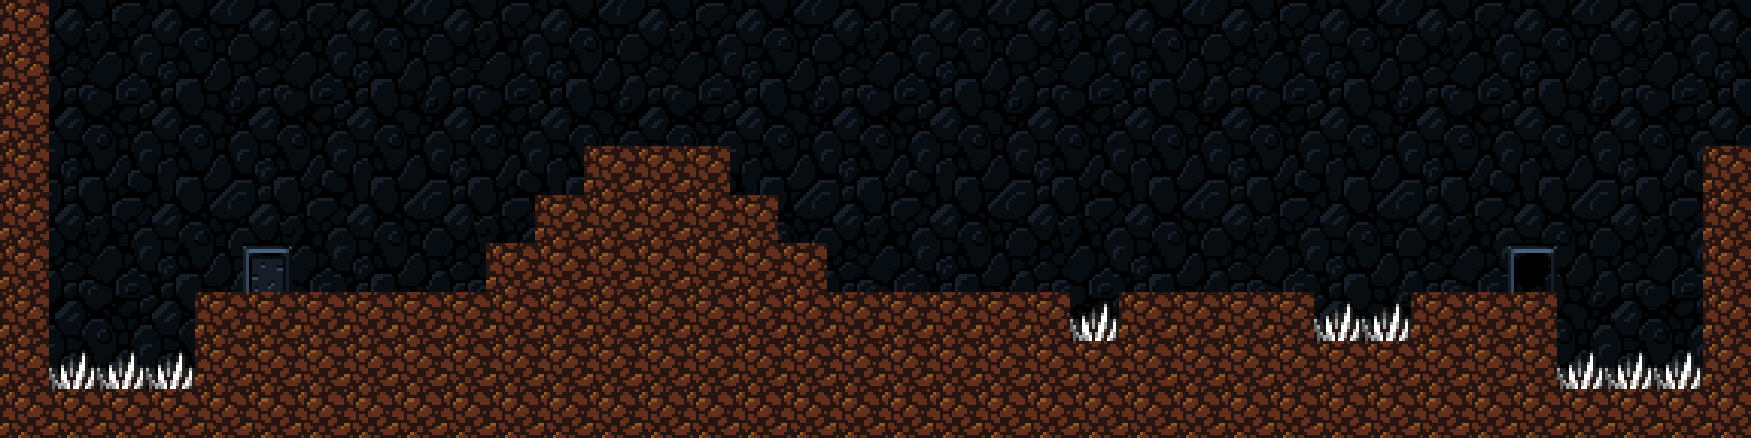
\includegraphics[width=\textwidth]{fig/levels/level1.pdf}
\caption{Cenário fácil, que explora o deslocamento horizontal do jogador.}
\label{fig:level1}
\end{figure}

O nível \textbf{médio}, além de explorar os elementos do nível \textit{fácil},
também requer que o jogador se desloque \textbf{verticalmente}. Esse nível é
mais difícil que o \textit{fácil} pois o jogador precisa \textbf{mudar de
direção} duas vezes. A figura \ref{fig:level2} mostra o nível médio, onde o
jogador deve se deslocar da entrada localizada na plataforma mais acima e à
esquerda até a saída que se encontra no canto direito e abaixo.

\begin{figure}[H]
\centering
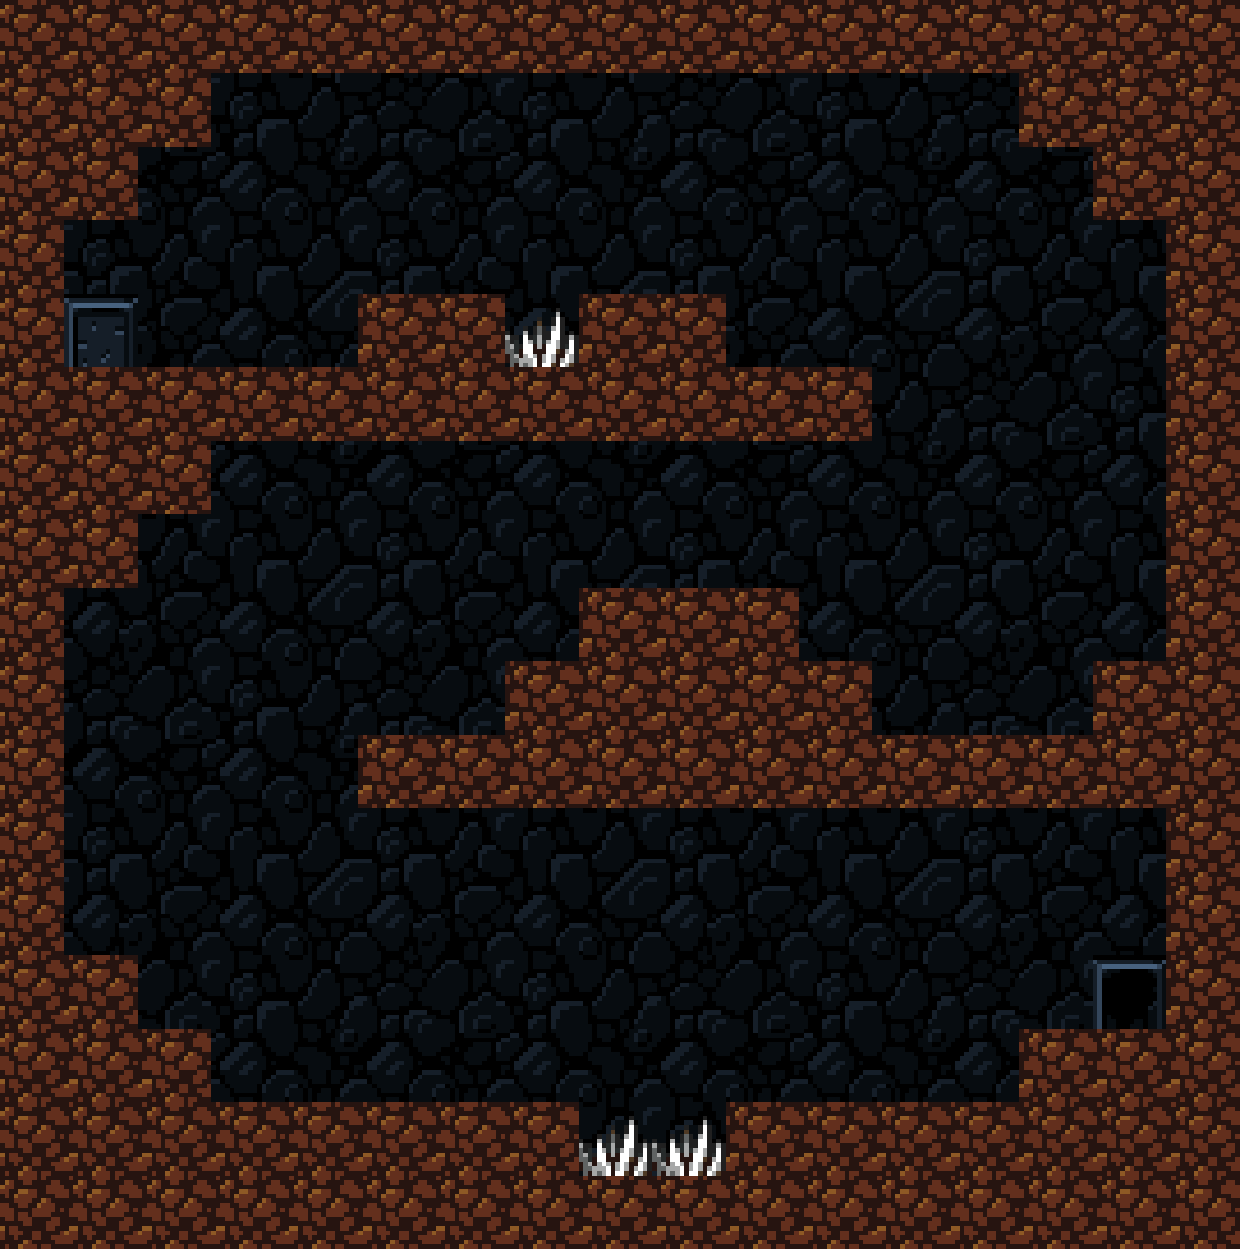
\includegraphics[width=\textwidth / 2]{fig/levels/level2.pdf}
\caption{Cenário médio, que explora o deslocamento horizontal e vertical do
    jogador, além de explorar a mudança de direção.}
\label{fig:level2}
\end{figure}

Para o nível médio, que conta com mais alguns desafios, estabelecemos os
seguintes \textbf{critérios de parada}:

\begin{description}
    \item [Número de execuções] no máximo \textbf{10000} execuções.
    \item [Tempo máximo de execução] no máximo \textbf{20 segundos} executando.
\end{description}

O nível \textbf{difícil} é um nível gerado aleatóriamente pelo jogo. Mesmo
sendo um nível gerado, é possível -- conforme a seção
\ref{section:spelunky-procgen-path} -- atravessar o nível sem a necessidade de
usar bombas, cordas ou outros equipamentos, sendo esse o desafio mais
interessante desse trabalho.

Por ser o cenário mais desafiador, estabelecemos os seguintes \textbf{critérios
de parada}:

\begin{description}
    \item [Número de execuções] no máximo \textbf{20000} execuções.
    \item [Tempo máximo de execução] no máximo \textbf{90 segundos} executando.
\end{description}

\section{Cenários Específicos}

Além dos desafios expostos nos níveis convencionais, existem alguns outros que
estão presentes em muitos níveis do jogo. Muitos deles requerem que alguns
botões sejam combinados ou pressionados em alguma sequência específica. Visando
explorar esses elementos, elaboramos alguns cenários para testes de situações
específicas.

Por serem cenários simplificados, elaboramos os seguintes \textbf{critérios de
parada} para todos eles:

\begin{description}
    \item [Número de execuções] no máximo \textbf{10000} execuções.
    \item [Tempo máximo de execução] no máximo \textbf{10 segundos} executando.
\end{description}

O cenário \textbf{extra 1}, exibido na figura \ref{fig:extra1}, conta com uma
escada que liga a plataforma inferior do jogo à plataforma superior. Portanto,
o jogador que deseja chegar até a porta de saída localizada na plataforma
superior deve fazer o uso dessa escada.

\begin{figure}[H]
\centering
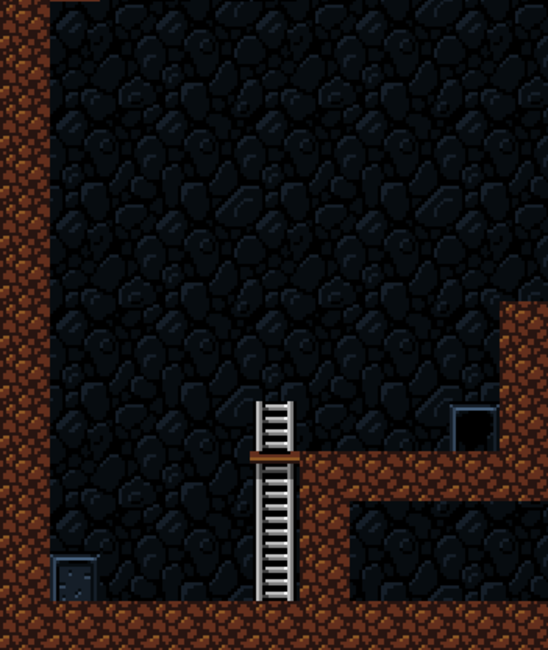
\includegraphics[width=\textwidth / 2]{fig/levels/extra1.pdf}
\caption{Cenário extra 1, que explora o uso de escadas por parte do jogador.}
\label{fig:extra1}
\end{figure}

Em alguns momentos, é necessário que o jogador se agarre à parede para poder
chegar até locais muito altos. Esse é um problema interessante, pois é
necessário a combinação das ações de movimentação e de salto. O nível
\textbf{extra 2} -- mostrado na figura \ref{fig:extra2} -- só pode ser vencido
caso o jogador salte, se agarre na parede e salte novamente, alcançando a
plataforma mais alta.

\begin{figure}[H]
\centering
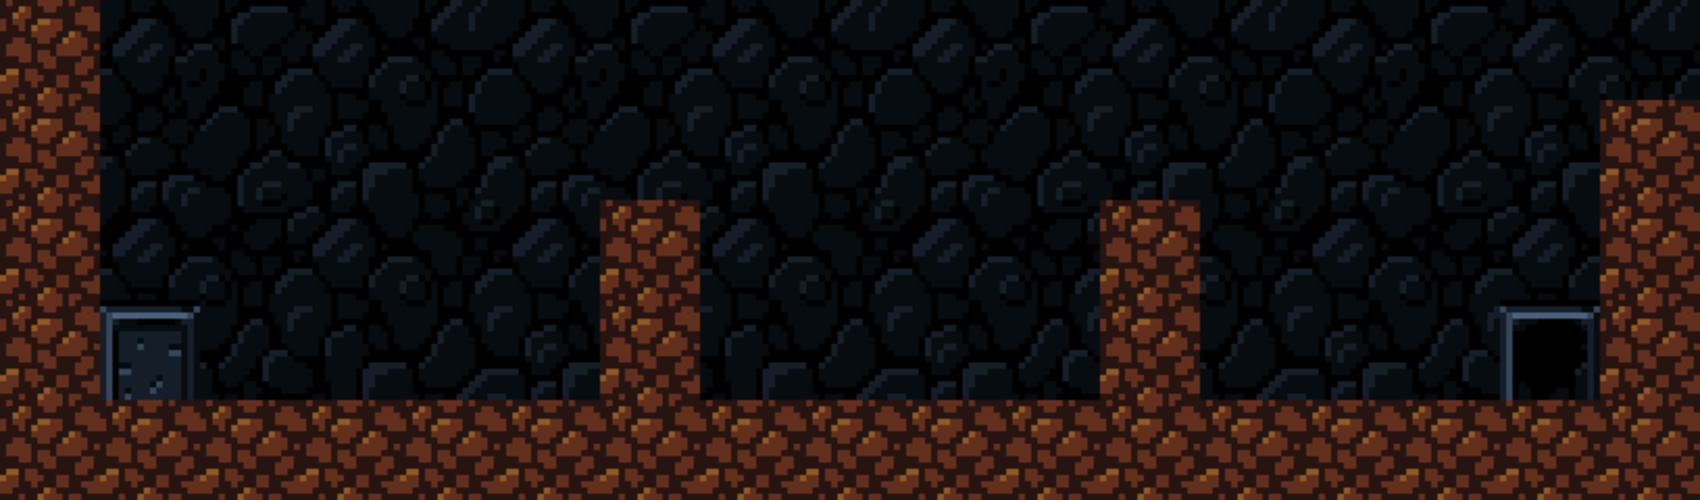
\includegraphics[width=\textwidth / 2]{fig/levels/extra2.pdf}
\caption{Cenário extra 2, que faz com que o jogador tenha que se agarrar à
    parede para vencer o nível.}
\label{fig:extra2}
\end{figure}

O jogo também conta com a possibilidade de \textbf{correr}, fazendo com que o
jogador se desloque mais rápido pelo nível. Além disso, quando o jogador corre,
é possível que este tenha uma impulsão maior no momento de saltar, podendo
passar por um número maior de obstáculos. De forma a explorar a corrida do
jogador, o nível \textbf{extra 3} -- representado na figura \ref{fig:extra3} --
só pode ser vencido se o jogador pular os espinhos enquanto estiver correndo.

\begin{figure}[H]
\centering
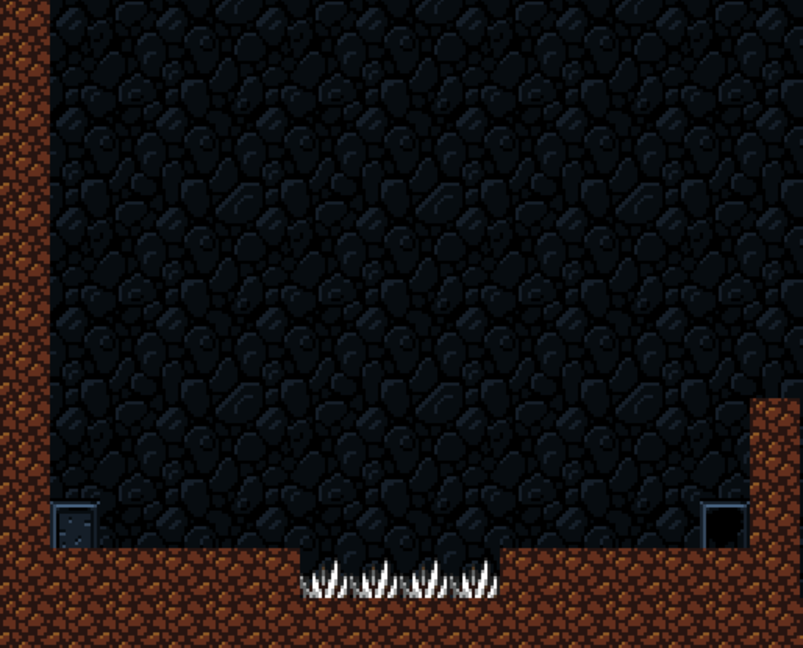
\includegraphics[width=\textwidth / 2]{fig/levels/extra3.pdf}
\caption{Cenário extra 3, que faz com que o jogador tenha que correr para
    vencer o nível.}
\label{fig:extra3}
\end{figure}

\todoin[caption={Cenários para Execução}] {
\begin{itemize}
	\item Mapas escolhidos:
	\begin{itemize}
		\item Easy (apenas alguns obstáculos)
		\item Medium (obstáculos e deslocamento vertical)
		\item Hard (mapa normal, gerado)
		\item Detalhar parâmetros de execução e critério de parada de cada mapa
	\end{itemize}

	\item Mapas adicionais (para teste de features):
	\begin{itemize}
		\item Motivação (tempo curto para explorar itens adicionais)
		\item Explorar corrida do bot
		\item Agarrando na parede
		\item Escadas
		\item Matar inimigos
		\item Coletar tesouros
		\item Detalhar parâmetros de execução e critério de parada de cada mapa
	\end{itemize}
\end{itemize}
}

\chapter{\label{chap:experimentation-and-results}Experimentação e Resultados Obtidos}

\todoin[caption={Experimentos Realizados}, color=cyan!60] {
    Experimentos:

	\begin{itemize}
        \item Inputs: visão, bias
        \item Outputs:
        \begin{itemize}
            \item convencionais: MOVIMENTACAO, PULO
            \item especificos: MOVIMENTACAO, PULO, EXTRA (depende do cenario)
        \end{itemize}
		\item Experimento \#1:fitness: AM, WAM, HM. Mapas: \textbf{easy}.
		\item Checkpoint: definir a fitness (WAM).

		\item Experimento \#2: rodar mapa medium com WAM
		\item Checkpoint: não vai funcionar (local ótimo)
		\item Checkpoint: adicionar novo input: \textbf{obstaculos}

		\item Experimento \#3: rodar mapa medium com WAM e novo input
		\item Checkpoint: funcionou, mas é um pouco problemático

		\item Experimento \#4: fitness exploratória (EX) com novo input
		\item Checkpoint: funcionou melhor

		\item Experimento \#5: janela de visão: 5x5, 7x7. Mapas: \textbf{medium}.
        \item Checkpoint: definir o tamanho da janela de visão.

        \item Experimento \#6: configurações de mutação. Mapas: \textbf{medium}.
        \item Checkpoint: definir configurações de mutação do NEAT.

		\item Experimento \#7: rodar mapa hard com as configurações definidas
		\item Checkpoint: ???

		\item Experimento \#7: experimentos nos cenários específicos
		\item Checkpoint: ???

		\item BONUS: fitness com A* ao invés de Manhattan Distance
		\item Checkpoint: ???
    \end{itemize}
	
    }

\todoin[caption={Detalhes}]{Introdução desse capítulo}

\section{\label{section:environment}Ambiente de Execução}

O capítulo \ref{chap:development} explica que faremos a execução do jogo em um
ambiente dedicado, utilizando o sistema operacional \textit{Linux}. Para isso,
utilizamos a plataforma \textit{Digital
Ocean}\footnote{https://www.digitalocean.com/}, que facilita a criação de uma
máquina para uso nesse trabalho. Além disso, essa plataforma permite alterar as
configurações -- quantidade de memória, número de processadores e quantidade de
armazenamento -- das máquina a qualquer momento, o que nos permitiu testar
diferentes configurações para o nosso problema.

Conforme explicado na seção \ref{sub:virtual-display}, fazemos o uso do
\textit{XVFB} para permitir a execução do jogo em um \textit{display} virtual. A
utilização de um \textit{display} virtual significa que necessitamos de uma
quantidade razoável de memória na máquina, sendo este um dos recursos mais
importantes para nós. Embora façamos a gravação de algumas informações em disco,
tratam-se apenas de arquivos de texto, que não ocupam uma grande quantidade de
espaço. Tendo isso em consideração, optamos por utilizar \textbf{3} máquinas,
com as configurações exibidas a seguir:

\begin{description}
    \item [Sistema Operacional] Ubuntu 16.04 - 64 \textit{bits}
    \item [Número de Processadores] 4
    \item [Modelo do Processador] Intel(R) Xeon(R) CPU E5-2630L v2 @ 2.40GHz
    \item [Quantidade de Memória] 4GB
    \item [Tipo de Disco] SSD
    \item [Quantidade de Disco] 60GB
\end{description}

Para automatizar o processo de configuração dessas máquinas, fizemos um
\textit{script} de instalação\footnote{https://github.com/famw/provisioning} de
todas as dependências para executar o projeto. Isto faz com que seja fácil
configurar uma nova máquina capaz de executar o treinamento dos agentes.

\section{\label{section:experiments}Experimentos Realizados}

\subsection{Escolha da Função de Aptidão}

\todoin[caption={Citar capítulo de modelagem}] {
    Citar capítulo de modelagem.
}

Conforme vimos no capítulo XYZ. A função de aptidão é o que determina a
\textbf{qualidade} da execução de um agente inteligente que utiliza algoritmos
genéticos. Portanto, é de extrema relevância experimentarmos diferentes valores
de aptidão para descobrirmos qual o que se encaixa melhor no nosso problema.

Assim, fizemos a execução do \textit{bot} no cenário \textbf{fácil} (Figura
\ref{fig:level1}, Capítulo \ref{chap:scenarios}) com três diferentes funções de
aptidão: \textbf{média aritmética}, \textbf{média aritmética ponderada} e
\textbf{média harmônica}. Obtivemos os resultados apresentados na Figura
\ref{fig:fitness-experiment}.

\begin{figure}[H]
\centering
	\begin{subfigure}[b]{0.4\textwidth}
        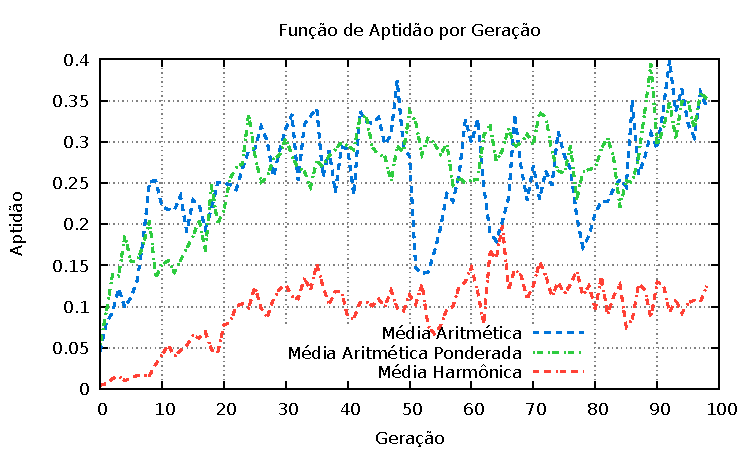
\includegraphics[width=\textwidth]{fig/fitness-value-comparison.pdf}
        \caption{Valor de aptidão em função do número de gerações para as
        diferentes funções de aptidão escolhidas.}
	\end{subfigure}
	\begin{subfigure}[b]{0.4\textwidth}
        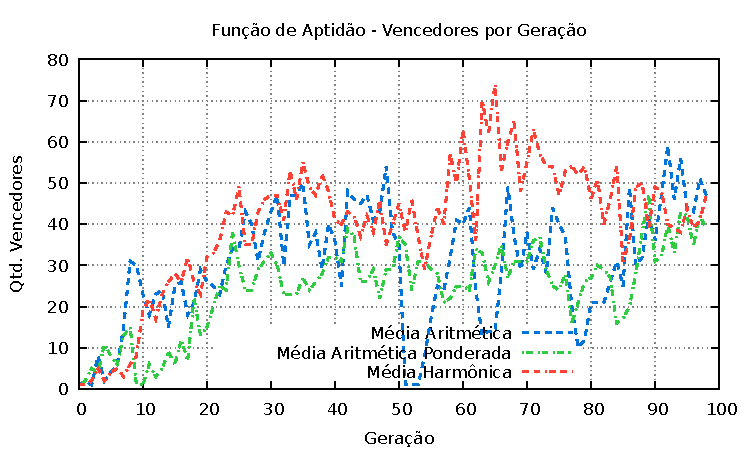
\includegraphics[width=\textwidth]{fig/fitness-winners-comparison.pdf}
        \caption{Número de organismos vencedores por geração para as diferentes
        funções de aptidão escolhidas.}
	\end{subfigure}

    \caption{Resultado da execução do cenário fácil com diferentes funções de
    aptidão.}
	\label{fig:fitness-experiment}
\end{figure}

Através da análise dos resultados, podemos ver que a \textbf{média
artimética} e a \textbf{média aritmética ponderada} têm um comportamento
muito semelhante, além de serem melhores do que a função de \textbf{média
harmônica}. Escolhemos então a \textbf{média aritmética ponderada} por ser
uma função que nos dá bastante controle sobre os valores que a compõem.
Embora a média harmônica tenha apresentado um comportamento bastante
estável, não a escolhemos  pois ela tem a característica de produzir
valores muito baixos quando algum dos seus termos apresenta um valor
pequeno, ou seja, esse valor acaba penalizando os outros. Isso pode fazer
com que algumas aptidões apresentem valores muito baixos, podendo
dificultar alguns treinamentos futuros.

\subsection{Adição de \textit{Input} de Obstáculo}

Com a função de aptidão escolhida, o próximo passo foi executar o \textit{bot}
em um nível mais desafiador que o nível \textbf{fácil}, portanto, executamos
ele no nível \textbf{médio}. Porém, percebemos que o jogador demorava muito
tempo para chegar até o final do nível. Acompanhando a execução, vimos que em
muitas gerações o \textit{bot} ia, no máximo, até o local indicado pela Figura
\ref{fig:experiment-medium-stuck}.

\begin{figure}[htb!]
\centering
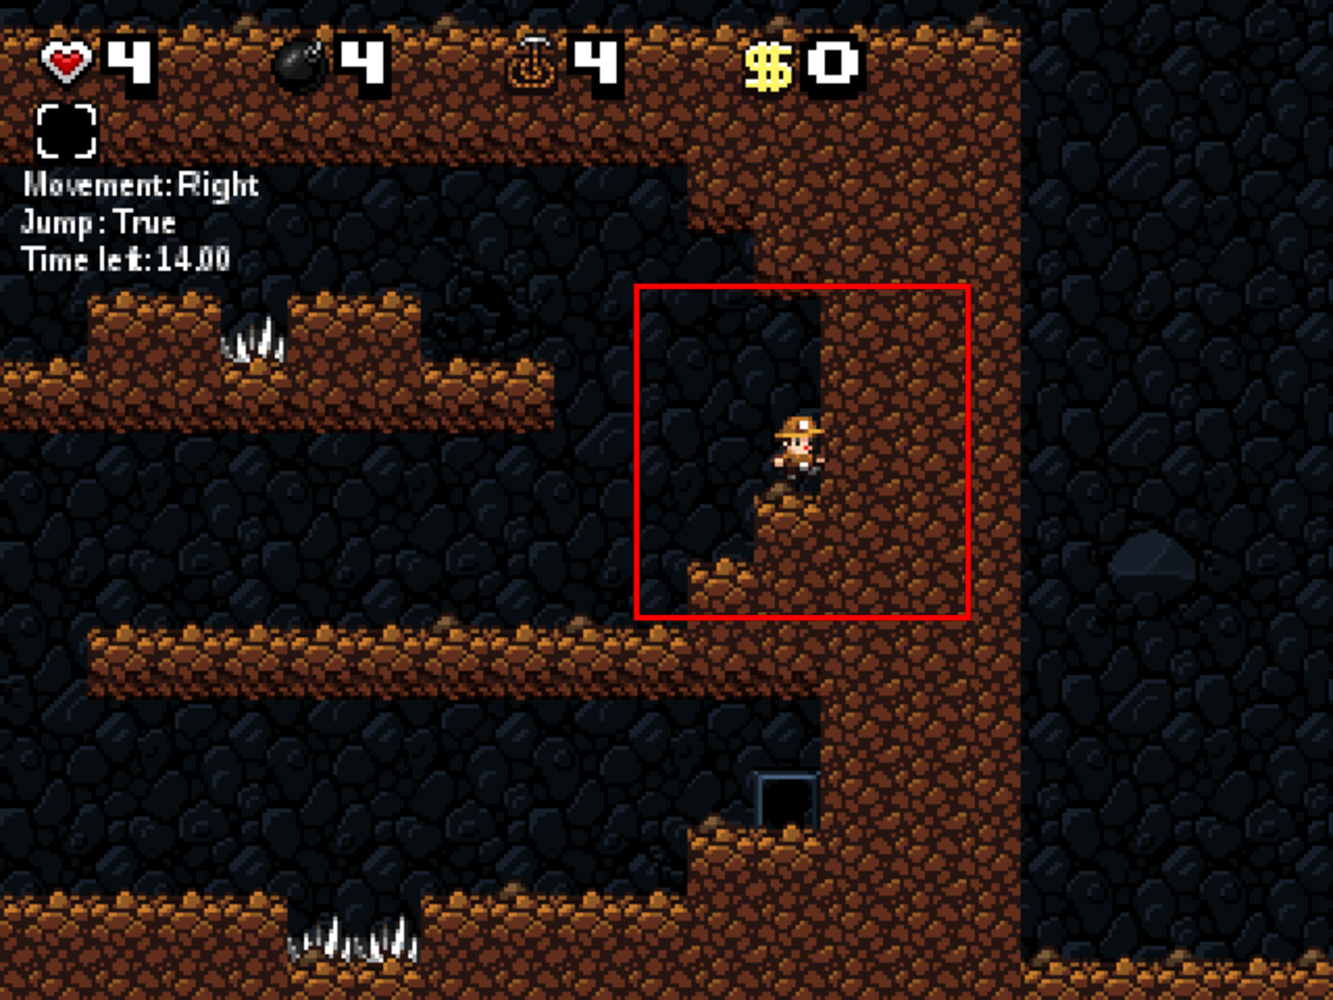
\includegraphics[width=.5\textwidth]{fig/experiment-medium-stuck.pdf}
\caption{Experimento mostrando o local onde o \textit{bot} fica parado ao
    executar no mapa médio com a média aritmética ponderada como função de
    aptidão.}
\label{fig:experiment-medium-stuck}
\end{figure}

Analisamos esse comportamento e percebemos que o \textit{bot} estava em um
local onde, naquele momento, ele considerava como \textit{ótimo}. Identificamos
isso pois nossa função de aptidão produz valores mais altos quanto maior for o
deslocamento horizontal e vertical do \textit{bot}. Dessa forma, caso ele fosse
para a esquerda, o valor de aptidão seria pior do que se ele ficasse parado
nesse local \textit{ótimo}. Um outro ponto importante é que é possível que as
mutações ou não estivessem ocorrendo ou não fossem suficientes para fazer com
que o \textit{bot} explorasse mais o mapa, de forma a fazer com que ele
entendesse que chegar na área inferior do mapa é mais vantajoso do que ficar
parado nesse local \textit{ótimo} por muitas gerações. O resultado dessa
execução pode ser visto na Figura \ref{fig:medium-wam-experiment}.

\begin{figure}[H]
\centering
	\begin{subfigure}[b]{0.4\textwidth}
        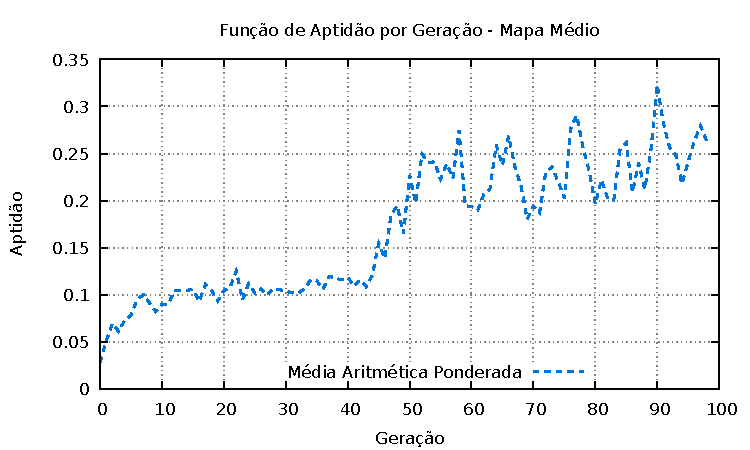
\includegraphics[width=\textwidth]{fig/medium-wam-fitness-experiment.pdf}
        \caption{Valor de aptidão em função do número de gerações para a média
        aritmética ponderada no mapa médio.}
	\end{subfigure}
	\begin{subfigure}[b]{0.4\textwidth}
        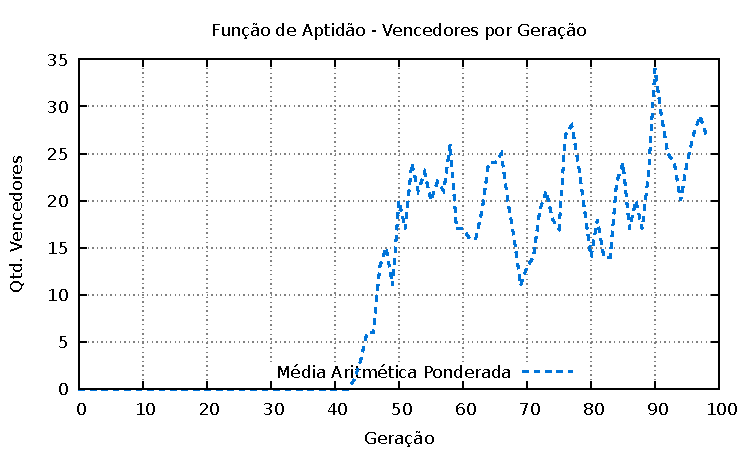
\includegraphics[width=\textwidth]{fig/medium-wam-winners-experiment.pdf}
        \caption{Número de organismos vencedores por geração para a média
        aritmética ponderada no mapa médio.}
	\end{subfigure}

    \caption{Resultado da execução do cenário médio com a média aritmética
    ponderada.}
	\label{fig:medium-wam-experiment}
\end{figure}

\todoin[caption={Citar capítulo de modelagem}] {
    Citar capítulo de modelagem.
}

Embora o \textit{bot} tenha vencido, ele demorou muito para isso -- após a
geração de número 40. Portanto, visando fazer com que ele aprendesse mais
rápido, adicionamos a entrada de \textit{obstáculo} na rede. O resultado dessa
modificação pode ser vista na Figura \ref{fig:medium-wam-obs-fitness-experiment}.

\begin{figure}[H]
\centering
	\begin{subfigure}[b]{0.4\textwidth}
        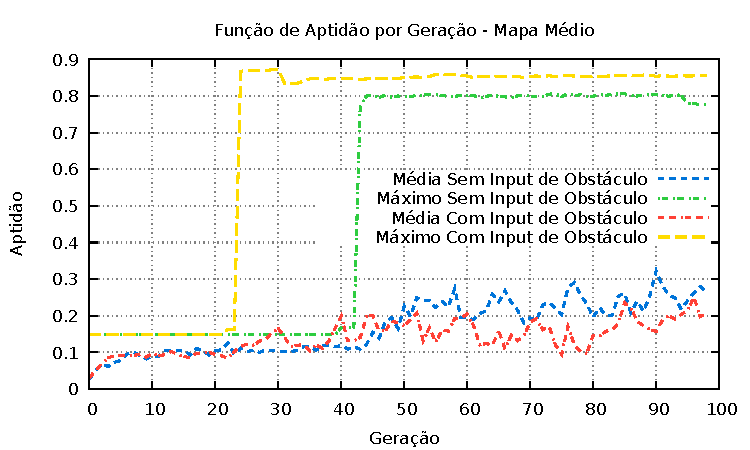
\includegraphics[width=\textwidth]{fig/medium-wam-obs-fitness-experiment.pdf}
        \caption{Valor de aptidão em função do número de gerações para a média
        aritmética ponderada, com o \textit{input} de obstáculo, no mapa
        médio.}
	\end{subfigure}
	\begin{subfigure}[b]{0.4\textwidth}
        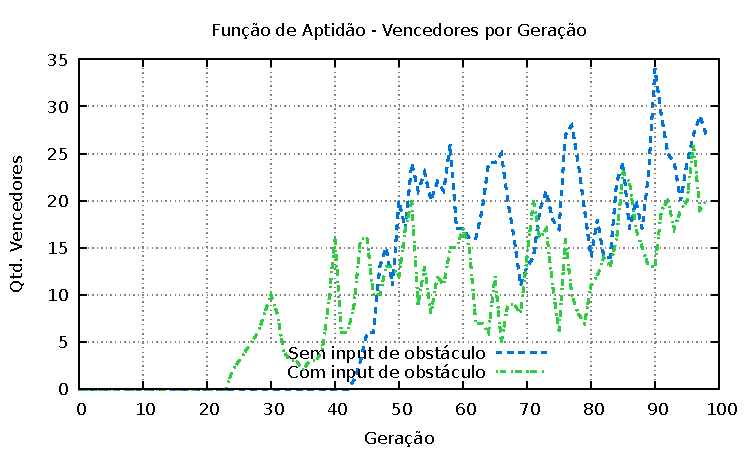
\includegraphics[width=\textwidth]{fig/medium-wam-obs-winners-experiment.pdf}
        \caption{Número de organismos vencedores por geração para a média
        aritmética ponderada, com o \textit{input} de obstáculo, no mapa
        médio.}
	\end{subfigure}

    \caption{Resultado da execução do cenário médio com a média aritmética
    ponderada.}
	\label{fig:medium-wam-obs-fitness-experiment}
\end{figure}

\todoin[caption={Melhorar análise dos resultados}, color=red!80] {
    Melhorar análise dos resultados.
}

\subsection{\label{section:experiment-vision}Tamanho da Janela de Visão}

\todoin[caption={Janela de Visão: Aguardando Resultados}, color=red!80] {
    Aguardando resultados.
}

\subsection{Configurações de Mutação}

\todoin[caption={Configurações de Mutação: Aguardando Resultados},
color=red!80] {
    Aguardando resultados.
}

\subsection{Execução no Cenário \textit{extra 1}}

\todoin[caption={Cenários Extra 1: Aguardando Resultados}, color=red!80] {
    Aguardando resultados.
}

\subsection{Execução no Cenário \textit{extra 2}}

\todoin[caption={Cenários Extra 2: Aguardando Resultados}, color=red!80] {
    Aguardando resultados.
}

\subsection{Execução no Cenário \textit{extra 3}}

\todoin[caption={Cenários Extra 3: Aguardando Resultados}, color=red!80] {
    Aguardando resultados.
}

\chapter{\label{chap:conclusion}Conclusão}

% Conclusion: here, you summarize what are your contributions and how you
% envision them going forward Contributions: what did you achieve in this work?
% Limitations: what are any problems or limitations to your contribution?
% Future work: what can be done to improve your work?

% ---------------------

% Texto extraído do capítulo de cenários por parecer fazer parte da conclusão:

% Os cenários anteriores exploram apenas a movimentação dos \textit{bots},
% porém, o jogo conta com outras características que podem ser exploradas em
% trabalhos futuros. De todas as possibilidades do jogo, as que julgamos mais
% importantes e que não exploramos nesse trabalho é a possibilidade de
% \textbf{matar inimigos} e \textbf{coletar tesouros}.

% Muitos mapas contam com inimigos no caminho do jogador, com isso, para ser
% possível vencer o nível, pode ser necessário abatê-los.  Assim, é
% interessante adicionarmos inimigos aos cenários, fazendo com que eles
% bloqueiem a passagem do jogador.

% Uma forma de se obter vantagens no jogo é através da \textbf{compra de
% itens}.  Os itens podem ser comprados com os tesouros obtidos ao longo do
% jogo. Dessa forma, também é interessante adicionarmos tesouros ao longo do
% caminho.

\todoin[caption={Conclusão}] {
	\begin{itemize}
        \item Dificuldades encontradas
        \item Falar o porquê de não termos conseguido executar no mapa hard
        \item Reforçar aqui o porquê de não termos utilizado behavior trees
            (citar todas as análises legais que fizemos)
		\item Relevância desse trabalho
        \item Contribuição para a computação/IA/Jogos
        \item O que esse trabalho contribuiu para nós
        \item Comparação com outros trabalhos
        \begin{itemize}
            \item Os outros trabalhos ``roubam'', o nosso não
        \end{itemize}
		\item Trabalhos futuros
		\begin{itemize}
            \item Possível reescrita do Spelunky/SpelunkBots, para não ter uma
                ``camada'' de \textit{view} atrelada, fazendo com que seja
                melhor de desenvolver IA's. Além disso, fazer essa reescrita
                visando ser multiplataforma e que seja mais eficiente.
            \item Acelerar a execução do spelunky/spelunkbots
            \item Considerar outros elementos do jogo, como inimigos, armas,
                tesouros, ferramentas e etc
			\item Visualizações dos treinamentos em real-time
		\end{itemize}
	\end{itemize}
}


\appendix
\chapter{\label{appendix:spelunkbots-variables}Lista de Variáveis Globais
de SpelunkBots}

\section{Movimentação do \textit{Bot}}
Estas são as variáveis \textit{booleanas} utilizadas para controlar quais botões
devem ser pressionados a cada etapa de execução, indicando aos \textit{bots}
quais ações devem executar:

\begin{center}
    \begin{tabular}{ |c| }
        \hline
        \textbf{Variável} \\ \hline
        global.attack \\ \hline
        global.duck \\ \hline
        global.goLeft \\ \hline
        global.goRight \\ \hline
        global.jump \\ \hline
        global.lookUp \\ \hline
        global.payp \\ \hline
        global.running \\ \hline
    \end{tabular}
\end{center}

\section{Tipo do Terreno}
Valores possíveis para os nodos de um mapa de \textit{Spelunky}:

\begin{center}
    \begin{tabular}{ |c|c| }
        \hline
        \textbf{Variável} & \textbf{Valor} \\ \hline
        global.spEmptyNode & 0 \\ \hline
        global.spStandardTerrain & 1 \\ \hline
        global.spLadder & 2 \\ \hline
        global.spEntrance & 3 \\ \hline
        global.spExit & 4 \\ \hline
        global.spSacAlter & 5 \\ \hline
        global.spArrowTrapRight & 6 \\ \hline
        global.spArrowTrapLeft & 7 \\ \hline
        global.spIsInShop & 8 \\ \hline
        global.spIce & 9 \\ \hline
        global.spSpike & 10 \\ \hline
        global.spSpearTrap & 11 \\ \hline
    \end{tabular}
\end{center}

\section{Inimigos e Armadilhas}
De modo similar aos valores de terreno, cada tipo de inimigo e armadilha possui
um valor de representação:

\begin{center}
    \begin{tabular}{ |c|c| }
        \hline
        \textbf{Variável} & \textbf{Valor} \\ \hline
        global.spGhost & 1 \\ \hline
        global.spBat & 2 \\ \hline
        global.spScarab & 3 \\ \hline
        global.spSpider & 4 \\ \hline
        global.spGiantSpiderHang & 5 \\ \hline
        global.spGiantSpider & 6 \\ \hline
        global.spFrog & 7 \\ \hline
        global.spFireFrog & 8 \\ \hline
        global.spZombie & 9 \\ \hline
        global.spVampire & 10 \\ \hline
        global.spPiranha & 11 \\ \hline
        global.spJaws & 12 \\ \hline
        global.spDeadFish & 13 \\ \hline
        global.spManTrap & 14 \\ \hline
        global.spMonkey & 15 \\ \hline
        global.spYeti & 16 \\ \hline
        global.spYetiKing & 17 \\ \hline
        global.spUFO & 18 \\ \hline
        global.spUFOCrash & 19 \\ \hline
        global.spAlienEject & 20 \\ \hline
        global.spAlien & 21 \\ \hline
        global.spAlienBoss & 22 \\ \hline
        global.spBarrierEmitter & 23 \\ \hline
        global.spBarrier & 24 \\ \hline
        global.spCaveman & 25 \\ \hline
        global.spHawkman & 26 \\ \hline
        global.spMagma & 27 \\ \hline
        global.spMagmaTrail & 28 \\ \hline
        global.spMagmaMan & 29 \\ \hline
        global.spTombLord & 30 \\ \hline
    \end{tabular}
\end{center}

\begin{center}
    \begin{tabular}{ |c|c| }
        \hline
        global.spOlmec & 31 \\ \hline
        global.spCavemanWorship & 32 \\ \hline
        global.spHawkmanWorship & 33 \\ \hline
        global.spOlmecDebris & 34 \\ \hline
        global.spSnake & 35 \\ \hline
        global.spSpiderHang & 36 \\ \hline
        global.spMagmaMan & 37 \\ \hline
        global.spShopkeeper & 38 \\ \hline
        global.spBones & 60 \\ \hline
        global.spSmashTrap & 61 \\ \hline
        global.spCeilingTrap & 62 \\ \hline
        global.spBoulder & 63 \\ \hline
        global.spSpringTrap & 99 \\ \hline
    \end{tabular}
\end{center}

\section{Objetos}
Existem diversos objetos em \textit{Spelunky} com os quais o jogador pode
interagir, e cada objeto é representado por um valor:

\begin{center}
    \begin{tabular}{ |c|c| }
        \hline
        \textbf{Variável} & \textbf{Valor} \\ \hline
        global.spGoldBar & 1 \\ \hline
        global.spGoldBars & 2 \\ \hline
        global.spEmerald & 3 \\ \hline
        global.spEmeraldBig & 4 \\ \hline
        global.spSapphire & 5 \\ \hline
        global.spSapphireBig & 6 \\ \hline
        global.spRuby & 7 \\ \hline
        global.spRubyBig & 8 \\ \hline
        global.spDiamond & 9 \\ \hline
        global.spGoldNugget & 10 \\ \hline
        global.spGoldChunk & 11 \\ \hline
        global.spChest & 12 \\ \hline
        global.spLockedChest & 13 \\ \hline
        global.spKey & 14 \\ \hline
        global.spCrate & 15 \\ \hline
        global.spFlareCrate & 16 \\ \hline
        global.spBombBag & 17 \\ \hline
        global.spBombBox & 18 \\ \hline
        global.spPaste & 19 \\ \hline
        global.spRopePile & 20 \\ \hline
        global.spParachute & 21 \\ \hline
        global.spCompass & 22 \\ \hline
        global.spSpringShoes & 23 \\ \hline
        global.spSpikeShoes & 24 \\ \hline
        global.spJordans & 25 \\ \hline
        global.spSpecs & 26 \\ \hline
        global.spUdjat & 27 \\ \hline
        global.spCrown & 28 \\ \hline
        global.spKapala & 29 \\ \hline
        global.spAnkh & 30 \\ \hline
        global.spGloves & 31 \\ \hline
        global.spMitt & 32 \\ \hline
        global.spJetpack & 33 \\ \hline
        global.spCape & 34 \\ \hline
        global.spRopeBag & 35 \\ \hline
    \end{tabular}
\end{center}

\section{Dados do Jogador}
Em adição às variáveis de controle, as variáveis de dados do jogador são
utilizadas para auxiliar o desenvolvedor a implementar o comportamento de um
\textit{bot}.

\begin{center}
    \begin{tabular}{ |c| }
        \hline
        \textbf{Variável (boolean)} \\ \hline
        global.hasGoal \\ \hline
        global.spIsInAir \\ \hline
        global.spIsJetpacking \\ \hline
        global.spJumpPressedPreviously \\ \hline
        global.itemGoal \\ \hline
        global.fogGoal \\ \hline
        global.endGoal \\ \hline
        global.headingRight \\ \hline
        global.headingLeft \\ \hline
        global.isPlayerHanging \\ \hline
        global.isPlayerHodldingHoldenIdol \\ \hline
    \end{tabular}
\end{center}

\begin{center}
    \begin{tabular}{ |c| }
        \hline
        \textbf{Variável (número inteiro)} \\ \hline
        global.playerPositionX \\ \hline
        global.playerPositionY \\ \hline
        global.playerPositionXNode \\ \hline
        global.playerPositionYNode \\ \hline
        global.pathCount \\ \hline
        global.tempID \\ \hline
        global.waitTimer \\ \hline
    \end{tabular}
\end{center}

\chapter{\label{appendix:spelunkbots-algorithms}Algoritmos Básicos Para
Implementação de \textit{Bots} Utilizando \textit{SpelunkBots}}

\section{Arquivo de \textit{Header}}

\begin{algorithm}[H]
\lstinputlisting[style=customC++]{code/ExampleBot.h}
\caption[Definição de métodos e variáveis de um \textit{bot} de exemplo.]
{\label{alg:project-example-bot-header}Definição de métodos e variáveis de um
\textit{bot} de exemplo.}
\end{algorithm}

\section{Implementação dos Métodos e Variáveis}

\begin{algorithm}[H]
\lstinputlisting[style=customC++]{code/ExampleBot.cpp}
\caption[Implementação dos métodos e variáveis de um \textit{bot} de exemplo.]
{\label{alg:project-example-bot-impl}Implementação dos métodos e variáveis de um
\textit{bot} de exemplo.}
\end{algorithm}

\chapter{\label{appendix:neat-configs}Arquivos de Exemplo de Configuração da
Biblioteca \textit{NEAT} Utilizada}

\section{Exemplo de Arquivo de Configurações de Mutação}
\begin{algorithm}[H]
\lstinputlisting[style=customC++]{code/neat_parameters_example.ne}
\caption[Exemplo de arquivo de configurações de mutação utilizado para
	parametrização da biblioteca de \textit{NEAT} utilizada.]
{\label{alg:neat-parameters-example}Exemplo de arquivo de configurações de
	mutação utilizado para parametrização da biblioteca de \textit{NEAT}
	utilizada.}
\end{algorithm}



\section{Exemplo de Arquivo de Rede Neural Inicial}
\begin{algorithm}[H]
\lstinputlisting[style=customC++]{code/neat_startgene_example}
\caption[Exemplo de arquivo de rede neural inicial utilizado para parametrização
	da biblioteca de \textit{NEAT} utilizada.]
{\label{alg:neat-network-example}Exemplo de arquivo de rede neural inicial
	utilizado para parametrização da biblioteca de \textit{NEAT} utilizada.}
\end{algorithm}




\bibliographystyle{tcc-num}
\bibliography{final-assignment-2-bib}

\end{document}
